\chapter{The fundamental group and some applications}
Algebraic topology assigns discrete algebraic invariants to topological spaces and continuous maps. More narrowly, one wants the algebra to be invariant with respect to continuous deformations of the topology. Typically, one associates a group $A(X)$ to a space $X$ and a homomorphism $A(p):A(X)\to A(Y)$ to a map $p:X\to Y$. We will write $A(p)$ as $p_*$.\par
In our context, a homotopy $h:p\simeq q$ between two maps $p,q:X\to Y$ is a continuous map $h:X\times I\to Y$ such that $h(x,0)=p(x)$ and $h(x,1)=q(x)$, where $I$ is the unit interval $[0,1]$. We usually want $p_*=q_*$ if $p\simeq q$, or some invariance property close to this.\par
In oversimplified outline, the way homotopy theory works is roughly this:
\begin{itemize}
\item One defines some algebraic construction $A$ and proves that it is suitably homotopy invariant.
\item One computes $A$ on suitable spaces and maps.
\item One takes the problem to be solved and deforms it to the point that step $2$ can be used to solve it.
\end{itemize}

\section{The fundamental group}
\subsection{Definitions of fundamental group}
\begin{definition}
Suppose $X$ and $Y$ are topological spaces and $f_0,f_1:X\to Y$ are two continuous functions. A homotopy from $f_0$ to $f_1$ is a continuous function
\[H:X\times I\to Y\]
such that
\[H(x,0)=f_0(x),\quad H(x,1)=f_1(x)\]
\end{definition}

We write $H:f_0\simeq f_1$ to indicate $H$ is a homotopy from $f_0$ to $f_1$, and we write $f_0\simeq f_1$ to indicate there exists such an $H$.\par

A homotopy defines a one-parameter family of continuous maps $H_t:X\to Y$ for $0\leq t\leq1$ by $H_t=H(x,t)$.

\begin{proposition}
Let $X$ and $Y$ denote two topological spaces. Then homotopy is an equivalence relation on the space $C(X,Y)$ of all continuous maps from $X$ to $Y$.
\end{proposition}
\begin{proof}
The only ponit need checking is the transitivity: if $F:f\simeq g$ and $G:g\simeq h$, define
\[H(x,t):=\begin{cases}
F(x,2t)&0\leq t\leq 1/2;\\
G(x,2t-1)&1/2\leq t\leq 1.
\end{cases}\]
Since $F$ and $G$ agree on their overlap, the pasting lemma implies that $H$ is continuous. Since $H(x,0)=f$ and $H(x,1)=h$, this shows that $f\simeq h$.
\end{proof}

We now show that composition of equivalence classes makes sense.

\begin{proposition}
Suppose $f_0,f_1:X\to Y$ and $g_0,g_1:Y\to Z$ are continuous functions with $f_0\simeq f_1$ and $g_0\simeq g_1$. Then $g_0\circ f_0\simeq g_1\circ f_1$, that is
\[[f_0]=[f_1]\text{ and }[g_0]=[g_1]\Rightarrow [g_0\circ f_0]=[g_1\circ f_1].\]
\end{proposition}
\begin{proof}
If fact we will show
\[[g_0\circ f_0]=[g_0\circ f_1]=[g_1\circ f_1].\]
Now suppose $F:f_0\simeq f_1$, $G:g_0\simeq g_1$. Define
\[H:X\times I\to Z,\quad H(x,t)=G(f_0(s),t).\]
Then $H$ is continuous and since
\[H(s,0)=G(f_0(s),0)=g_0(f_0(s)),\quad H(s,1)=G(f_0(s),1)=g_1(f_0(s)).\]
This gives the first equality, the other can be done similarly.
\end{proof}

Let $X$ and $Y$ be topological spaces, and $A\sub X$ an arbitrary subset. A homotopy $H$ between maps $f,g:X\to Y$ is said to be \textbf{stationary on $\bm{A}$} if
\[H(x,t)=f(x),\quad\forall x\in A,t\in I.\]
In other words, for each $t$, the map $H_t$ agrees with $f$ on $A$. If there exists such a homotopy $H$, we say that $f$ and $g$ are homotopic relative to $A$, and $H$ is also called \textbf{a homotopy relative to $\bm{A}$}. Notice that this implies $g|_A=H|_A=f|_A$, so for two maps to be homotopic relative to $A$ they must first of all agree on $A$. Sometimes, for emphasis, when two maps are homotopic but the homotopy is not assumed to be
stationary on any particular subspace, we say they are \textbf{freely homotopic}, and the homotopy is a \textbf{free homotopy}.

\begin{definition}
Let $X$ be a space, two paths $f,g:I\to X$ from $p$ to $q$ are equivalent if they are homotopic through paths from $p$ to $q$. That is, there exist a homotopy $H:I\times I\to X$ such that
\[H(s,0)=f(s),\quad H(s,1)=g(s),\quad H(0,t)=p,\text{ and}\quad H(1,t)=q.\]
for all $s,t\in I$.
\end{definition}

Note the additional condition we impose: the end points of two paths should be fixed by our homotopy, This is to avoid some trivial occasions, and such kind of homotopy is sometimes called \textbf{path homotopy}. Write $[f]$ for the equivalence class of $f$. We say that $f$ is a \textbf{loop} if $f(0)=f(1)$. If $f$ is a loop whose initial and terminal point is $p\in X$, we say that $f$ is \textbf{based at $\bm{p}$}, and we call $p$ the base point of $f$. The set of all loops in $X$ based at $p$ is denoted by $\Omega(X,p)$. The constant loop $c_p\in\Omega(X,p)$ is the map $c_p(s)=p$. A \textbf{null-homotopic loop} is one that is path-homotopic to a constant loop, not just homotopic.\par 
Define $\pi_1(X,p)$ to be the set of equivalence classes of loops that start and end at $p$. And define the product operation on paths: For paths $f,g:I\to X$ such that $f(1)=g(0)$, define $f\ast g$ as
\[(f\ast g)(s)=\begin{cases}
f(2s)&\text{if }0\leq s\leq 1/2;\\
g(2s-1)&\text{if }1/2\leq s\leq 1.
\end{cases}\]
And $\bar{f}$ to be the opposite path $\bar{f}(s)=f(1-s)$.\par 
The product operation on paths induces a well-defined operation on path-homotopy classes, defined by the equation
\[[f]\ast[g]:=[f\ast g].\]
This is well defined as the reader will check. Moreover, after passage to equivalence classes, this composition becomes associative and unital. Although direct verification is easy, it is more illuminating to draw a picture of the domain squares and to indicate schematically how the homotopies are to behave on it. In the following, we assume given paths
\[f,g,h:I\to X.\]
To prove the equations
\[f\ast(g\ast h)\simeq (f\ast g)\ast h,\quad f\ast c_x\simeq f,\quad c_x\ast f\simeq f.\]
consider following homotopies:
\[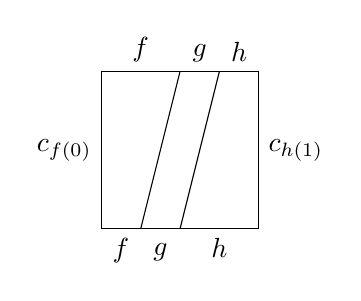
\begin{tikzpicture}[scale=2]
\draw (0,0) rectangle (1,1);
\node[below] at (0.125,0) {$f$};
\node[below][below,yshift=-2pt] at (0.375,0) {$g$};
\node[below] at (0.75,0) {$h$};

\node[above] at (0.25,1) {$f$};
\node[above] at (0.625,1) {$g$};
\node[above] at (0.875,1) {$h$};

\node[left] at (0,0.5) {$c_{f(0)}$};
\node[right] at (1,0.5) {$c_{h(1)}$};

\draw (0.25,0)--(0.5,1)
(0.5,0)--(0.75,1);
\end{tikzpicture}\quad\quad\quad\begin{tikzpicture}[scale=2]
\draw (0,0) rectangle (1,1);
\node[below] at (0.25,0) {$c_{f(0)}$};
\node[below] at (0.75,0) {$f$};

\node[above] at (0.5,1) {$f$};

\node[left] at (0,0.5) {$c_{f(0)}$};
\node[right] at (1,0.5) {$c_{f(1)}$};

\draw (0.5,0)--(0,1);
\end{tikzpicture}\quad\quad\quad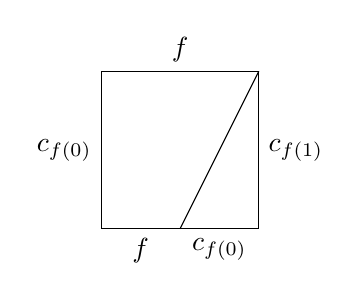
\begin{tikzpicture}[scale=2]
\draw (0,0) rectangle (1,1);
\node[below] at (0.75,0) {$c_{f(0)}$};
\node[below] at (0.25,0) {$f$};

\node[above] at (0.5,1) {$f$};

\node[left] at (0,0.5) {$c_{f(0)}$};
\node[right] at (1,0.5) {$c_{f(1)}$};

\draw (0.5,0)--(1,1);
\end{tikzpicture}\]
Moreover, $[\bar{f}\ast f]=[c_{f(0)}]$ and $[f\ast\bar{f}]=[c_{f(1)}]$. For the first, we have the following schematic picture and corresponding formula. In the schematic picture,
\[f_t=f|[0,t]\And \bar{f}_t=\bar{f}|[1-t, 1].\]
\[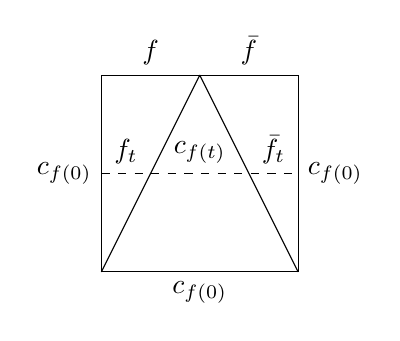
\begin{tikzpicture}[scale=2.5]
\draw (0,0) rectangle (1,1);
\node[below] at (0.5,0) {$c_{f(0)}$};

\node[above] at (0.25,1) {$f$};
\node[above] at (0.75,1) {$\bar{f}$};

\node[left] at (0,0.5) {$c_{f(0)}$};
\node[right] at (1,0.5) {$c_{f(0)}$};

\node[above] at (0.125,0.5) {$f_t$};
\node[above] at (0.875,0.5) {$\bar{f}_t$};
\node[above] at (0.5,0.5) {$c_{f(t)}$};
\draw (0,0)--(0.5,1)
(1,0)--(0.5,1);
\draw[dashed](0,0.5)--(1,0.5);
\end{tikzpicture}\]
\[h(s,t)=\begin{cases}
f(2s)&\text{if }0\leq s\leq t/2;\\
f(t)&\text{if }t/2\leq s\leq 1-t/2;\\
f(2-2s)&\text{if }1-t/2\leq s\leq 1.
\end{cases}\]
We conclude that $\pi_1(X,p)$ is a group with identity element $e=[c_p]$ and inverse elements $[f]^{-1}=[\bar{f}]$. It is called the \textbf{fundamental group} of $X$, or the first \textbf{homotopy group} of $X$.
\begin{remark}
The reader should view paths as continuous maps from a special sapce to $X$, i.e., the unit interval $I$. And loops are maps from $S^1$ to $X$. These ideas give the generalization of the fundemental group, which is, homotopy groups of higher order. They are maps from $S^n$ to $X$, modulo the homotopy relation.
\end{remark}
\begin{remark}[Dependence on the basepoint]
For a path $g:I\to X$ be a path from $p$ to $q$, define a \textbf{change-of-basepoint} map $\varPhi_{g}:\pi_1(X,p)\to\pi_1(X,q)$ by \[\varPhi_{g}[f]=[g]^{-1}\ast[f]\ast[g]=[\bar{g}\ast f\ast g].\]
It is easy to check that $\varPhi_{g}$ depends only on the equivalence class of $g$ and is a homomorphism of groups. For a path $g':q\to r$, we see that \[\varPhi_{g\ast g'}=\varPhi_{g'}\circ\varPhi_{g}.\]
It follows that $\varPhi_{g}$ is an isomorphism with inverse $\varPhi_{\bar{g}}$.\par
If the group $\pi_1(X,p)$ happens to be Abelian, which may or may not be the case, then this is just $[f]$. Then we see that, when $\pi_1(X,p)$ is Abelian, $\varPhi_{g}$ is independent of the choice of the path class $[a]$:
\[\varPhi_{g}[f]=[\bar{g}]\ast[f]\ast[g]=[f].\]
Thus, in this case, we have a canonical way to identify $\pi_1(X,p)$ with $\pi_1(X,q)$.
\end{remark}
\subsection{Circle Representatives}
Let $\omega:I\to S^1$ denote the loop given in complex notation by
\[\omega(s)=e^{2\pi is}.\]
If $f:I\to X$ is any loop in a space $X$, it passes to the quotient to give a unique map $\widetilde{f}:S^1\to X$ such that $\widetilde{f}=f\circ\omega$, which we call the \textbf{circle representative} of $f$. Conversely, any continuous map $\widetilde{f}$ from the circle to $X$ is the circle representative of the map $f=\widetilde{f}\circ\omega$.\par
The next proposition gives a convenient criterion for detecting null-homotopic loops in terms of their circle representatives.
\begin{proposition}\label{null homotopy iff}
Let $X$ be a topological space. Suppose $f:I\to X$ is a loop based at $p\in X$, and $\widetilde{f}:S^1\to X$ is its circle representative. Then the following are equivalent.
\begin{itemize}
\item[$(a)$] $f$ is a null-homotopic loop.
\item[$(b)$] $\widetilde{f}$ is freely homotopic to a constant map.
\item[$(c)$] $\widetilde{f}$ extends to a continuous map from the closed disk into $X$.
\end{itemize}
\end{proposition}
\begin{proof}
We prove that $(a)\Rightarrow(b)\Rightarrow(c)\Rightarrow(a)$. Suppose first that $f$ is null-homotopic, and let $H:I\times I\to X$ be a path homotopy between $f$ and the constant loop $c_p$. The map $\omega\times id:I\times I\to S^1\times I$ is a quotient map by the closed map lemma, and $H$ respects the identifications made by this map. Thus it descends to a map $\widetilde{H}:S^1\times I\to X$, which is easily seen to be a homotopy between $\widetilde{f}$ and the constant map sending $S^1$ to $p$.\par
Next, assume that $\widetilde{f}$ is freely homotopic to a constant map $k:S^1\to X$, and let $H:S^1\times I\to X$ be a homotopy with $H_0=k$ and $H_1=f$. Recall that the quotient space $CS^1=S^1\times I/(S^1\times\{0\})$(the cone on $S^1$) is homeomorphic to $\widebar{\B}^2$. The map $H$ takes $S^1\times\{0\}$ to a single point, so it descends to the quotient to yield a continuous map $\widetilde{H}:\widebar{\B}^2\approx CS^1\to X$. Because the quotient map restricts to the obvious identification $S^1\times\{1\}\approx S^1\hookrightarrow\widebar{\B}^2$, it follows that the
restriction of $\widetilde{H}$ to $S^1$ is equal to $\widetilde{f}$.\par
Finally, assume that $\widetilde{f}$ extends to a continuous map $F:\widebar{\B}^2\to X$. Because $\widetilde{\B}^2$ is convex, we can form the straight-line homotopy from the constant loop $c_1$ to the loop $\iota_{S^1}\circ\omega:I\to S^1\hookrightarrow\widebar{\B}^2$; call it $H:I\times I\to\widebar{\B}^2$. Because $H(s,t)\in S^1$ when $(s,t)\in\partial(I\times I)$, the composite map $F\circ H:I\times I\to X$ satisfies
\[F\circ H(s,0)=\widetilde{f}\circ H(s,0)=\widetilde{f}\circ c_1(s)=p.\]
\[F\circ H(s,0)=\widetilde{f}\circ H(s,1)=\widetilde{f}\circ\omega(s)=f(s).\]
\[F\circ H(0,t)=\widetilde{f}\circ H(0,t)=\widetilde{f}(1)=p.\]
\[F\circ H(1,t)=\widetilde{f}\circ H(1,t)=\widetilde{f}(1)=p.\]
and is therefore a path homotopy from $c_p$ to $f$.
\end{proof}
\begin{lemma}[\textbf{Squre lemma}]\label{squre lem}
Let $F:I\times I\to S$ be a continuous map, and let $f$, $g$, $h$, and $k$ be the paths in $X$ defined by
\[f(s)=F(s,0),\quad g(s)=F(1,s),\quad h(s)=F(0,s),\quad k(s)=F(s,1)\]
Then $f\ast g\simeq h\ast k$.
\[\begin{tikzpicture}[scale=2]
\draw (0,0) rectangle (1,1);
\node[below] at (0.5,0) {$f$};

\node[above] at (0.5,1) {$k$};

\node[left] at (0,0.5) {$h$};

\node[right] at (1,0.5) {$g$};
\end{tikzpicture}\]
\end{lemma}
\begin{proof}
Choose a homeomorphism $\varphi:I\times I\to\widebar{\B}^2$ which maps the four pieces of boundaries to the four quardant of $S^1$. Denote $\pi:S^1\to X$ to be the path obtained by travelling around $\partial(I\times I)$. Then $\pi$ is the circle representative of $f\ast g\ast\bar{h}\ast\bar{k}$. Since $\pi$ extends to a continuous map $\widetilde{F}:\widebar{\B}^2\to X$, by Proposition~\ref{null homotopy iff} $f\ast g\ast\bar{h}\ast\bar{k}$ is null homotopic. So $f\ast g\simeq h\ast k$.
\end{proof}
\subsection{Fundamental Groups of Spheres}
The $n$-sphere minus the north pole is homeomorphic to $\R^n$ by stereographic projection. In fact, composing the stereographic
projection with a suitable rotation of the sphere shows that the sphere minus
any point is homeomorphic to $\R^n$. Therefore, if we knew that every loop in $S^n$ omitted at least one point in the sphere, we could consider it as a loop in $\R^n$; since it is null-homotopic there, it is null-homotopic in $S^n$.\par
Unfortunately, an arbitrary loop might not omit any points. For example, there is a continuous surjective map $f:I\to I\times I$. Composing this with a quotient map $I\times I\to S^2$ yields a path whose image is all of $S^2$. But as we will show below, we can modify any loop by a homotopy so that it does miss a point.\par
The key is a tool that allows us to break up maps from $I$ (or indeed any compact metric space) into smaller pieces.
\begin{lemma}
Suppose $M$ is a manifold of dimension $n\geq2$. If $f$ is a path in $M$ from
$p_1$ to $p_2$ and $q$ is any point in $M$ other than $p_1$ or $p_2$, then $f$ is path-homotopic to a path that does not pass through $q$.
\end{lemma}
\begin{proof}
Consider the open cover $\{U,V\}$ of $M$, where $U$ is a coordinate ball centered at $q$ and $V=M\setminus\{q\}$. If $f:I\to M$ is any path from $p_1$ to $p_2$, then $\{f^{-1}(U),f^{-1}(V)\}$ is an open cover of $I$. Let $\delta$ be a Lebesgue number for this cover, and let $m$ be a positive integer such that $1/m<\delta$. It follows that on each subinterval $[k/m,(k+1)/m]$, $f$ takes its values either in $U$ or in $V$. If $f(k/m)=q$
for some $k$, then the two subintervals $[(k-1)/m,k/m]$ and $[k/m,(k+1)/m]$ must both be mapped into $U$. Thus, letting $0=a_0<\cdots<a_l=1$ be the points of the form $k/m$ for which $f(a_i)\neq q$, we obtain a sequence of curve segments $f|_{[a_{i-1},a_i]}$ whose images lie either in $U$ or in $V$, and for which $f(a_i)\neq q$.\par
Now, $U\setminus\{q\}$ is homeomorphic to $\B^n\setminus\{0\}$, which is path-connected. (Here is where the dimensional restriction comes in: when $n=1$, $\B^n\setminus\{0\}$ is disconnected.) Thus, for each such segment that lies in $U$, there is another path in $U\setminus\{q\}$ with the same endpoints; since $U$ is simply connected, these two paths are path-homotopic
in $U$ and thus in $M$. Of course, each segment that lies in $V$ already misses $q$.
\end{proof}
\begin{theorem}
For $n\geq 2$, $S^n$ is simply connected.
\end{theorem}
\begin{proof}
Let $N\in S^n$ be the north pole, and choose any base point $p\in S^n$ other than $N$. If $f:I\to S^n$ is any loop based at $p$, the preceding lemma shows that $f$ is pathhomotopic in $S^n$ to a loop in $S^n\setminus\{N\}$. Since $S^n\setminus\{N\}\approx\R^n$, $f$ is null-homotopic in $S^n\setminus\{N\}$ and therefore also in $S^n$.
\end{proof}
\subsection{Fundamental Groups of Manifolds}
The Lebesgue number lemma also allows us to prove an important theorem about fundamental groups of manifolds.
\begin{theorem}
The fundamental group of a manifold is countable.
\end{theorem}
\begin{proof}
Let $M$ be a manifold, and let $\mathcal{U}$ be a countable cover of $M$ by coordinate balls. For each $U$, $U'\in\mathcal{U}$, the intersection $U\cap U'$ has at most countably many components; choose a point in each such component and let $\mathcal{X}$ denote the (countable) set consisting of all the chosen points as $U$, $U'$ range over all the sets in $\mathcal{U}$. For each $U\in\mathcal{U}$ and $x$, $x'\in\mathcal{X}$ such that $x,x'\in U$, choose a definite path $h^U_{x,x'}$ from $x$ to $x'$ in $U$.\par
Now choose any point $p\in\mathcal{X}$ as base point. Let us say that a loop based at $p$ is \textbf{special} if it is a finite product of paths of the form $h^U_{x,x'}$. Because both $\mathcal{U}$ and $\mathcal{X}$ are countable sets, there are only countably many special loops. Each special loop determines an element of $\pi_1(M,p)$. If we can show that every element of $\pi_1(M,p)$ is obtained in this way, we are done, because we will have exhibited a surjective map from a countable set onto $\pi_1(M,p)$.\par
So suppose $f$ is any loop based at $p$. By the Lebesgue number lemma there is an integer $n$ such that $f$ maps each subinterval $[(k-1)/n,k/n]$ into one of the balls in $\mathcal{U}$; call this ball $U_k$. Let $f_k=f|_{[(k-1)/n,k/n]}$ reparametrized on the unit interval, so that $[f]=[f_1]\ast\cdots\ast[f_n]$.\par
For each $k=1,\cdots,n-1$, the point $f(k/n)$ lies in $U_k\cap U_{k+1}$. Therefore, there is some $x_k\in\mathcal{X}$ that lies in the same component of $U_k\cap U_{k+1}$ as $f(k/n)$. Choose a path $g_k$ in $U_k\cap U_{k+1}$ from $x_k$ to $f(k/n)$, and set $\widetilde{f}_k=g_{k-1}\ast f_k\ast \bar{g}_k$ (taking $x_k=p$ and $g_k$ to be the constant path $c_p$ when $k=0$ or $n$). It is immediate that $[f]=[f_1]\ast\cdots\ast[f_n]$, because all the $g_k's$ cancel out. But for each $k$, $\widetilde{f}_k$ is a path in $U_k$ from $x_{k-1}$ to $x_k$, and since $U_k$ is simply connected, $\widetilde{f}_k$ is path-homotopic to $h^{U_k}_{x_{k-1},x_k}$. This shows that $f$ is path-homotopic to a special loop and completes the proof.
\begin{figure}[htbp]
\centering
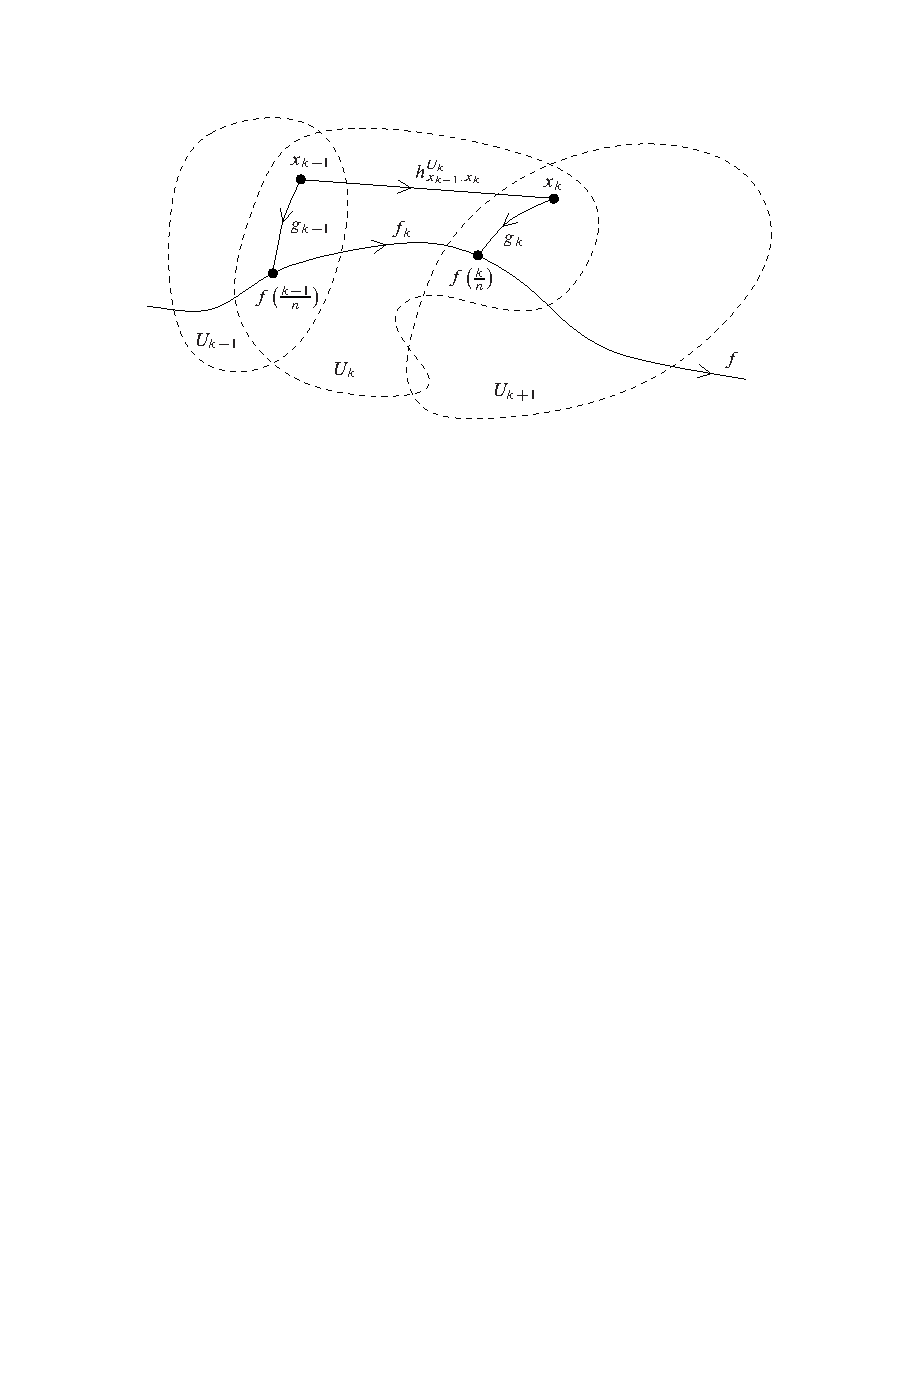
\includegraphics{pictures/fandamental-group-of-manifold}
\caption{Proof that a manifold has countable fundamental group.}
\end{figure}
\end{proof}

\subsection{Homotopy invariance}
\begin{proposition}
The path homotopy relation is preserved by composition with continuous maps. That is, if $f_0$, $f_1:I\to X$ are path-homotopic and $\varphi:X\to Y$ is continuous, then $\varphi\circ f_0$ and $\varphi\circ f_1$ are path-homotopic.
\end{proposition}
For a map $\varphi:X\to Y$, define $\pi_1(\varphi):\pi_1(X,x)\to\pi_1(Y,\varphi(x))$ by 
\[\varphi_*[f]=[\varphi\circ f],\]
where $\varphi\circ f$ is the composite of $\varphi$ with the loop $f:I\to X$. Clearly $\varphi_*$ is a homomorphism. The identity map $id:X\to X$ induces the identity homomorphism. For a map $\psi:Y\to Z$, we have
\[(\psi\circ \varphi)_*=\psi_*\circ \varphi_*.\]
so this functor acts covariantly.
\begin{proposition}
Homeomorphic spaces have isomorphic fundamental groups. Specifically, if $\varphi:X\to Y$ is a homeomorphism, then $\varphi_*:\pi_1(X,p)\to\pi_1(Y,\varphi(p))$ is an isomorphism.
\end{proposition}
There is one case in which the homomorphism induced by inclusion
can be easily shown to be injective. 
\begin{definition}
Let $X$ be a space and $A\sub X$ a subspace. A continuous map $r:X\to A$ is called a \textbf{retraction} if the restriction of $r$ to $A$ is the identity map of $A$, or equivalently if $r|_A=id_A$. If there exists a retraction from $X$ to $A$, we say that $A$ is a \textbf{retract} of $X$.
\end{definition}
\begin{proposition}
Suppose $A$ is a retract of $X$. If $r:X\to A$ is any retraction,
then for any $p\in A$, $(\iota_A)_*:\pi_1(A,p)\to\pi_1(X,p)$ is injective and $r_*:\pi_1(X,p)\to\pi_1(A,p)$ is surjective.
\end{proposition}
\begin{proof}
Since $r\circ\iota_A=id_A$, the composition $r_*\circ(\iota_A)_*$ is the identity on $\pi_1(A,p)$, from which it follows that $(\iota_A)_*$ is injective and $r_*$ is surjective.
\end{proof}
\begin{corollary}\label{retract simply connected}
A retract of a simply connected space is simply connected.
\end{corollary}
Here are some examples of retractions. For these examples we use the as yet
unproved fact that the circle is not simply connected.
\begin{example}
For any $n\geq1$, it is easy to check that the map $r:\R^n\setminus\{0\}\to S^{n-1}$ given by $r(x)=x/|x|$ is a retraction. Because $S^1$ is not simply connected, it follows from Corollary~\ref{retract simply connected} that $R^2\setminus\{0\}$ is not simply connected. Thus $\R^2\setminus\{0\}$ is not
homeomorphic to $\R^2$.
\end{example}
\begin{example}
The torus $T^2=S^1\times S^1$ has a subspace $A=S^1=\{1\}$ homeomorphic to $S^1$, and the map $r:T^2\to A$ given by $r(s,t)=(s,1)$ is easily seen to be a retraction. Thus $T^2$ is not simply connected, so it is not homeomorphic
to $S^2$.
\end{example}
\begin{example}
For a simple example, we claim $\pi_1(\R,0)=0$.\par
In fact, define $H:\R\times I\to\R$ by $H(s,t)=(1-t)s$. Then $H$ is a homotopy
from the identity to the constant map at $0$. For a loop $f:I\to\R$ at $0$, define $G(s,t)=H(f(s),t)$. The homotopy $G$ shows that $f$ is equivalent to $c_0$.
\end{example}
\begin{example}
Consider the circle $S^1$ to be the set of complex numbers $z=x+iy$ of norm $1$. Observe that $S^1$ is a group under multiplication of complex numbers. It is a topological group: multiplication is a continuous function. We take the identity element $1$ as a convenient basepoint for $S^1$. Then we claim
\[\pi_1(S^1,1)\simeq\Z.\]
We may postpone this proof until we have the concept of covering sapces.
\end{example}
\subsection{Homotopy Equivalence}
Let $\varphi:X\to Y$ be a continuous map. We say that another continuous map
$\psi:Y\to X$ is a \textbf{homotopy inverse} for $\varphi$ if $\psi\circ\varphi\simeq id_X$ and $\varphi\circ\psi\simeq id_Y$. If there exists a homotopy inverse for $\varphi$, then $\varphi$ is called a \textbf{homotopy equivalence}. In this case, we say that $X$ is \textbf{homotopy equivalent} to $Y$, or $X$ has the same \textbf{homotopy type}
as $Y$, and we write $X\simeq Y$. Properties that are preserved by homotopy equivalences are called \textbf{homotopy invariants}.\par
Suppose $X$ is a topological space, $A$ is a subspace of $X$, and $r:X\to A$ is a retraction.We say that $r$ is a \textbf{deformation retraction} if $\iota_A\circ r$ is homotopic to the identity map of $X$, where $\iota_A:A\to X$ is the inclusion map. If there exists a deformation retraction from $X$ to $A$, then $A$ is said to be a \textbf{deformation retract} of $X$. Because $\iota_A\circ r\simeq id_X$ and $r\circ\iota_A=id_A$, it follows that both $\iota_A$ and $r$ are homotopy equivalences.\par
Most deformation retractions that arise in practice are of the following special type. A retraction $r:X\to A$ is called a \textbf{strong deformation retraction} if $id_X$ is homotopic to $\iota_A\circ r$ relative to $A$, which means that there is a homotopy from $id_X$ to $\iota_A\circ r$ that is stationary on $A$. In this case, we say that $A$ is a \textbf{strong deformation retract} of $X$.\par
Unwinding the definitions, we see that a space $A\sub X$ is a deformation retract of $X$ if and only if there exists a homotopy $H:X\times I\to X$ that satisfies
\[H(x,0)=x,\ \forall x\in X\quad H(x,1)\in A,\ \forall x\in X\quad H(a,1)=a,\ \forall a\in A.\]
For a strong deformation retract, the third condition is replaced by
\[H(a,t)=a,\ \forall a\in A, t\in I.\]
Given such a homotopy, the map $r:X\to A$ defined by $r(x)=H(x,1)$ is a (strong) deformation retraction. Thus to say that $A$ is a deformation retract of $X$ is to say that $X$ can be continuously deformed into $A$, with points of $A$ ending up where they started. It is a strong deformation retract if the points of $A$ remain fixed throughout the deformation.\par
Because the existence of the homotopy is the essential requirement for showing
that a subspace is a deformation retract, it is common in the literature to use the term \textit{deformation retraction} to refer to the homotopy $H$ rather than the retraction $r$, and we sometimes do so when convenient; it should be clear from the context whether the term refers to the retraction or the homotopy.
\begin{proposition}
For any $n\geq 1$, $S^{n-1}$ is a strong deformation retract of $\R^n\setminus\{0\}$ and of $\widebar{\B}^n\setminus\{0\}$.
\end{proposition}
\begin{proof}
Define a homotopy $H:(\R^n\setminus\{0\})\times I\to\R^n\setminus\{0\}$ by
\[H(x,t)=(1-t)x+t\dfrac{x}{|x|}.\]
\end{proof}
\begin{corollary}
For $n\geq 3$, both $\R^n\setminus\{0\}$ and $\widebar{\B}^n\setminus\{0\}$ are simply connected.
\end{corollary}
\begin{example}
If $n\geq1$ and $D\sub\R^n$ is a compact convex subset with nonempty
interior, then Proposition~\ref{CW compact convex is n-cell} show that $\partial D$ is homotopy equivalent to both $\R^n\setminus\{p\}$ and $D\setminus\{p\}$ where $p\in\Int D$.
\end{example}
\begin{example}
Let $X$ be any space. If the identity map of $X$ is homotopic to a constant map, we say that $X$ is \textbf{contractible}. Other equivalent definitions are that any point of $X$ is a deformation retract of $X$, or $X$ is homotopy equivalent to a one-point space. Concretely, contractibility means that there exist a point $p\in X$ and a continuous map $H:X\times I\to X$ such that
\[H(x,0)=x,\quad H(x,1)=p\]
In other words, the whole space $X$ can be continuously shrunk to a point. Some
simple examples of contractible spaces are convex subsets of $\R^n$, and, more generally, any subset $B\sub\R^n$ that is \textbf{star-shaped}, which means that there is some point $p_0\in B$ such that for every $p\in B$, the line segment from $p_0$ to $p$ is contained in $B$. Since a one-point space is simply connected, it follows that every contractible space is simply connected.
\end{example}
Note that if $X$ is contractible, it is not necessarily the case that each point of $X$ is a strong deformation retract of $X$.\par
if two maps $F_0$ and $F_1$ are homotopic, we have no guarantee that both maps take the base point $p\in X$ to the same point in $Y$, so their induced homomorphisms do not even map into the same group. The following rather complicated-looking lemma is a substitute for the claim that homotopic maps induce the same fundamental group homomorphism. It says, in effect, that homotopic maps induce the same homomorphism up to a canonical change of base point.
\begin{lemma}\label{homotopic map incude}
Suppose $\varphi,\psi:X\to Y$ are continuous, and $H:\varphi\simeq\psi$ is a homotopy. For any $p\in X$, let $h$ be the path in $Y$ from $\varphi(p)$ to $\psi(p)$ defined by $h(t)=H(x,t)$, and let $\varPhi_h:\pi_1(Y,\varphi(p))\to\pi_1(Y,\psi(p))$ be the isomorphism. Then the following diagram commutes:
\[\begin{tikzcd}
&\pi_1(Y,\varphi(p))\ar[dd,"\varPhi_h"]\\
\pi_1(X,p)\ar[ru,"\varphi_*"]\ar[rd,swap,"\psi_*"]&\\
&\pi_1(Y,\psi(p))\\
\end{tikzcd}\]
\end{lemma}
\begin{proof}
Let $f$ be any loop in $X$ based at $p$. What we need to show is
\begin{align*}
&\psi_*[f]=\varPhi_h(\varphi_*[f])\\
&\iff\psi\circ f\simeq\bar{h}\ast(\varphi\circ f)\ast h\\
&\iff h\ast(\psi\circ f)\simeq (\varphi\circ f)\ast h.
\end{align*}
This follows easily from the square lemma applied to the map $F:I\times I\to Y$ defined by $F(s,t)=H(f(s),t)$.
\end{proof}
\begin{corollary}
Suppose $\varphi,\psi: X\to Y$ are continuous maps and $H:\varphi\simeq\psi$ is a homotopy. Suppose $p\in X$ has the property that $\varphi(p)=\psi(p)$. Set $q:=\varphi(p)$. Then $\varphi_*$ and $\psi_*$ are \textbf{conjugate group homomorphisms}, that is, there exists $[w]\in\pi_1(Y,q)$ such that
\[\varphi_*[u]=[w]^{-1}\ast \psi_*[u]\ast[w],\quad \forall[u]\in\pi_1(X,p).\]
\end{corollary}
\begin{corollary}
Suppose $X$ and $Y$ are connected topological spaces, and the fundamental group of $Y$ is abelian. If $\varphi,\psi:X\to Y$ are homotopic maps such that $\varphi(p)=\psi(p)$ for some $p\in X$, then $\varphi_*=\psi_*:\pi_1(X,p)\to\pi_1(Y,\varphi(p))$.
\end{corollary}
Our main goal in this section is the following theorem, which is a much stronger invariance property than homeomorphism invariance, and will enable us to compute the fundamental groups of many more spaces.
\begin{theorem}[\textbf{Homotopy Invariance of $\bm{\pi_1}$}]\label{homotopy Inva of pi_1}
If $\varphi:X\to Y$ is a homotopy equivalence, then for any point $p\in X$, $\varphi_*:\pi_1(X,p)\to\pi_1(Y,\varphi(p))$ is an isomorphism.
\end{theorem}
\begin{proof}
Suppose $\varphi:X\to Y$ is a homotopy equivalence, and let $\psi:Y\to X$ be a homotopy inverse for it. Consider the sequence of maps
\begin{equation}\label{homotopy Inva of pi_1-1}
\begin{tikzcd}\pi_1(X,p)\ar[r,"\varphi_*"]&\pi_1(Y,\varphi(p))\ar[r,"\psi_*"]&\pi_1(X,\psi\circ\varphi(p))\ar[r,"\varphi_*"]&\pi_1(Y,\varphi\circ\psi\circ\varphi(p))
\end{tikzcd}
\end{equation}
We need to prove that the first $\varphi_*$ above is bijective. As we mentioned earlier, $\psi_*$ is not an inverse for it, because it does not map into the right group.\par
Since $\psi\circ\varphi\simeq id_X$, Lemma~\ref{homotopic map incude} shows that there is a path $h$ in $X$ such that the following diagram commutes:
\[\begin{tikzcd}
&\pi_1(X,\varphi(p))\ar[dd,"\varPhi_h"]\\
\pi_1(X,p)\ar[ru,"(id_X)_*"]\ar[rd,swap,"(\psi\circ\varphi)_*"]&\\
&\pi_1(X,\psi\circ\varphi(p))\\
\end{tikzcd}\]
Thus
\begin{align}\label{homotopy Inva of pi_1-2}
\psi_*\circ\varphi_*=\varPhi_h.
\end{align}
which is an isomorphism. In particular, this means that the first $\varphi_*$ in $(\ref{homotopy Inva of pi_1-1})$ is injective and $\psi_*$ is surjective.\par
Similarly, the homotopy $\varphi\circ\psi\simeq id_Y$ leads to the diagram
\[\begin{tikzcd}
&\pi_1(Y,\varphi(p))\ar[dd,"\varPhi_h"]\\
\pi_1(Y,\varphi(p))\ar[ru,"(id_Y)_*"]\ar[rd,swap,"(\varphi\circ\psi)_*"]&\\
&\pi_1(Y,\varphi\circ\psi\circ\varphi(p))\\
\end{tikzcd}\]
from which it follows that $\varphi_*\circ\psi_*$ is an isomorphism. This means in particular that $\psi_*$ is injective; since we already showed that it
is surjective, it is an isomorphism. Therefore, going back to $(\ref{homotopy Inva of pi_1-2})$, we conclude that $\varphi_*=(\psi_*)^{-1}\circ\varPhi_h$ is also an isomorphism.
\end{proof}
Let $X$ and $Y$ be topological spaces, and let $f:X\to Y$ be a continuous map.
Define the \textbf{mapping cylinder} $Z_f$ of $f$ to be the adjunction space $Y\cup_\varphi(X\times I)$, where the attaching map $\varphi:X\times\{0\}\to Y$ is given by $\varphi(x,0)=f(x)$.\par
The subspace $X\times\{1\}\sub Y\amalg(X\times I)$ is a saturated closed subset homeomorphic to $X$. The restriction of the quotient map $q\to Y\amalg(X\times I)\to Z_f$ to this subset is thus a one-to-one quotient map, so its image $\widetilde{X}$ is also homeomorphic to $X$. Similarly, $\widetilde{Y}=q(Y)$ is homeomorphic to $Y$.
\begin{proposition}
With notation as above, if $f$ is a homotopy equivalence, then $\widetilde{Y}$
and $\widetilde{X}$ are deformation retracts of $Z_f$. Thus two spaces are homotopy equivalent if and only if they are both homeomorphic to deformation retracts of a single space.
\end{proposition}
\begin{proof}
For any $(x,s)\in X\times I$, let $[x,s]=q(x,s)$ denote its equivalence class in $Z_f$; similarly, $[y]=q(y)$ is the equivalence class of $y\in Y$.
First we show that $\widetilde{Y}$ is a strong deformation retract of $Z_f$, \textbf{assuming only that $\bm{f}$ is continuous}. We define a retraction $A:Z_f\to Z_f$, which collapses $Z_f$ down onto $\widetilde{Y}$, by
\[A[x,s]=[x,0],\quad A[y]=[y].\]
To be a bit more precise, we should define a map $\widetilde{A}: Y\amalg(X\times I)\to Z_f$ by $\widetilde{A}(x,s)=[x,0]$ and $\widetilde{A}(y)=[y]$ . This map is evidently continuous because its restrictions to $X\times I$ and $Y$ are compositions of continuous maps. Because $\widetilde{A}(x,0)=[f(x)]=\widetilde{A}(f(x))$, $\widetilde{A}$ respects the identifications made by $q$, so it passes to the quotient to yield the continuous map $A$ defined above. In this proof, we use this kind
of standard argument repeatedly to show that a map from $Z_f$ is continuous; we
generally abbreviate it by saying something like $A$ is well defined and continuous because $A[x,0]=[f(x)]=A[f(x)]$.\par
Define a homotopy $H_1:Z_f\times I\to Z_f$ by
\[H_1([x,s],t)=[x,s(1-t)],\quad H_1([y],t)=[y].\]
Because $H_1([x,0],t)=[x,0]=[f(x)]=H_1([f(x),0],t)$, $H_1$ is well defined. To
check that it is continuous, we need only observe that it respects the identifications made by the map $q\times id_I:(Y\amalg(X\times I))\times I\to Z_f\times I$, which is a quotient map. Since $H_1(\xi,0)=\xi$ and $H_1(\xi,1)=A(\xi)$ for any $\xi\in Z_f$ , $H_1$ is a homotopy between the identity map of $Z_f$ and $A$. Since, moreover, $H_1([y],t)=[y]$ for all $y\in Y$, it is in fact a strong deformation retraction.\par
Now suppose $f$ is a homotopy equivalence, and let $g:Y\to X$ be a homotopy
inverse for it. Thus there exist homotopies $F:Y\times I\to X$ and $G:X\times I\to X$ such that $F:f\circ g\simeq\id_Y$ and $G:g\circ f\simeq\id_X$. Define two more 
homotopies $H_2$ and $H_3$ by
\[H_2([x,s],t)=[F(f(x),1-t)],\quad H_2([y],t)=[F(y,1-t)].\]
\[H_3([x,s],t)=[G(x,st),t],\quad H_3([y],t)=[g(y),t].\]
It is clear that $H_2$ and $H_3$ are well defined and continuous. Geometrically, $H_2$ deforms all of $Z_f$ into the image of $f$ in $\widetilde{Y}$ along the homotopy $F$, and then $H_3$ collapses $Z_f$ onto $\widetilde{X}$ by deforming each point along the homotopy $G$.\par
Inserting $t=0$ and $t=1$ into the definitions of $H_2$ and $H_3$, we find that $H_2:A\simeq B$ and $H_3:B\simeq C$, where
\[B[x,s]=[g(f(x)),0],\quad B[y]=[g(y),0].\]
\[C[x,s]=[G(x,s),1],\quad C[y]=[g(y),1].\]
Because homotopy is transitive, the three homotopies $H_1$, $H_2$, $H_3$ yield $\id_{Z_f}\simeq A\simeq B\simeq C$. Since $G(x,1)=x$, we find that $C[x,1]=[x,1]$, so $C$ is a retraction onto $\widetilde{X}$, which shows that $\widetilde{X}$ is a deformation retract of $Z_f$.
\begin{figure}[htbp]
\centering
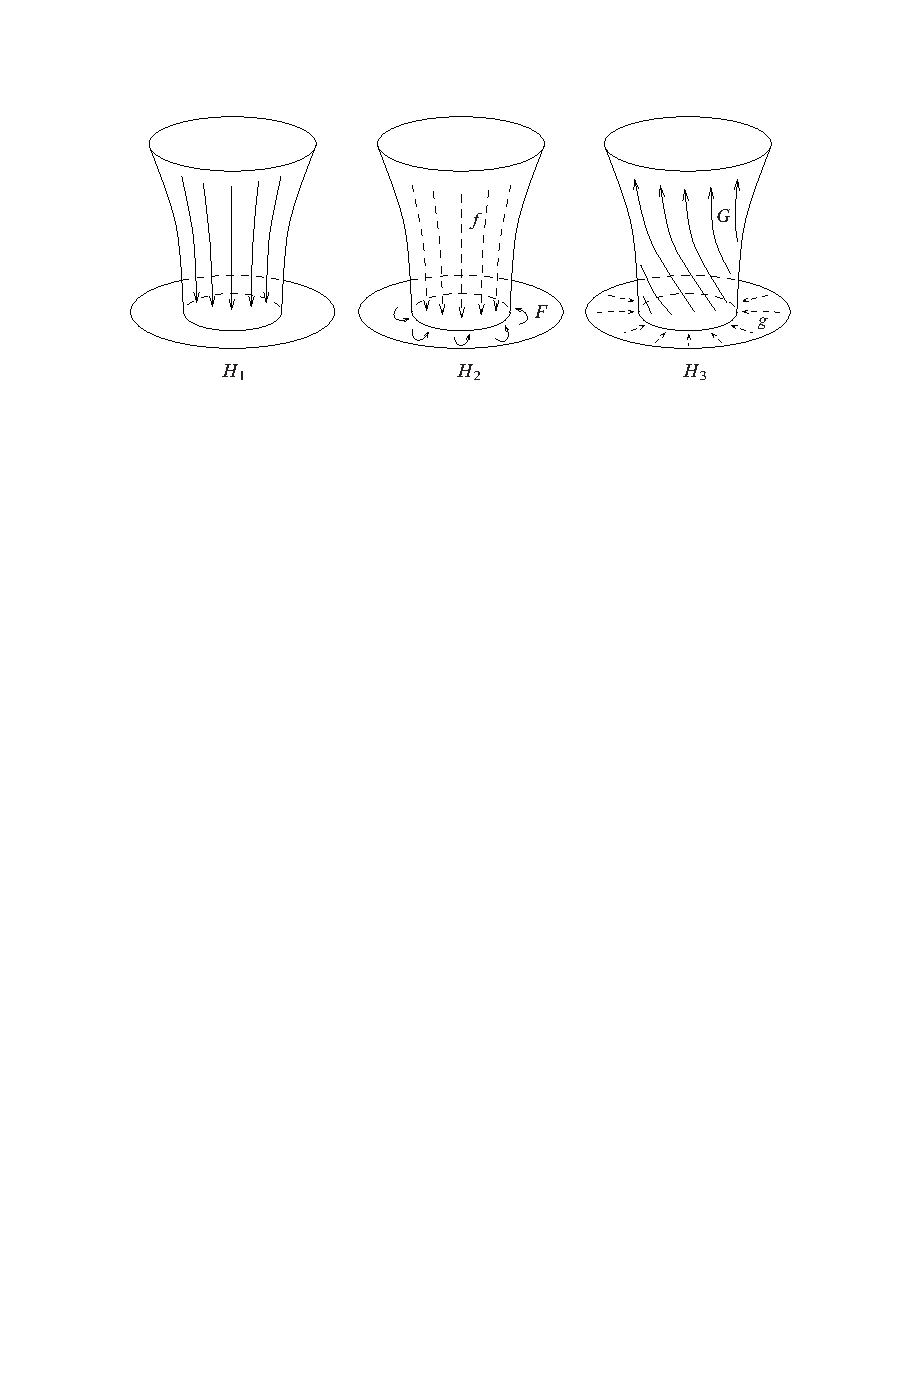
\includegraphics{pictures/retraction}
\caption{Homotopies of the mapping cylinder.}
\end{figure}
\end{proof}
\subsection{Degree Theory for the Circle}
Suppose $f:I\to S^1$ is a loop based at a point $z_0\in S^1$. If $\widetilde{f}:I\to\R$ is any lift of $f$, then $\widetilde{f}(0)$ and $\widetilde{f}(1)$ are both points in the fiber $p^{-1}(z_0)$, so they differ by an integer. Since any other lift differs from $\widetilde{f}$ by an additive constant, the difference $\widetilde{f}(1)-\widetilde{f}(0)$ is an integer that depends only on $f$, and not on the choice of lift. This integer is denoted by $N(f)$, and is called the \textbf{winding number} of $f$.
\begin{theorem}[\textbf{Homotopy Classification of Loops in $\bm{S^1}$}]
Two loops in $S^1$ based at the same point are path-homotopic if and only if they have the same winding number.
\end{theorem}
If $\varphi:S^1\to S^1$ is a continuous map, we define the \textbf{degree} of $\varphi$ to be the winding number of the loop $\varphi\circ\omega$, where $\omega:I\to S^1$ is the standard generator of $\pi_1(S^1,1)$, that is, $\omega(s)=e^{2\pi is}$. This integer is denoted by $\deg\varphi$.\par
Or we can define the degree of a map $\varphi$ to be the image of the generator of $\pi_1(S^1,1)$ under $\varphi_*$. But this needs $\varphi(1)=1$ so that $\varphi_*$ maps $\pi_1(S^1,1)$ to itself. For maps that do not
preserve the base point, we define its degree by considering the composition
\[\begin{tikzcd}
\pi_1(S^1,1)\ar[r,"\varphi_*"]&\pi_1(S^1,\varphi(1))\ar[r,"\varPhi_{g}"]&\pi_1(S^1,1)
\end{tikzcd}\]
which sends $\omega$ to $\deg\varphi\cdot\omega$. Here $g$ is any path $f(1)\to 1$ because $\varPhi_{g}$ is independent of the choice of $[\alpha]$ since $\pi_1(S^1,1)$ is Abelian. And for convention, we use the unique rotation that takes $\varphi(1)$ to $1$, and denote it by $\rho_\varphi$. That is, $\rho_\varphi(z)=z/\varphi(1)$.
\begin{proposition}[\textbf{Properties of the Degree}]\label{degree prop}
\mbox{}
\begin{itemize}
\item[$(a)$] Homotopic continuous maps have the same degree.
\item[$(b)$] If $\varphi,\psi:S^1\to S^1$ are continuous maps, then $\deg(\psi\circ\varphi)=(\deg\psi)(\deg\varphi)$.
\end{itemize}
\end{proposition}
\begin{proof}
We begin with $(a)$. Assume that $\varphi,\psi:S^1\to S^1$ are homotopic continuous maps. Then
\[\deg\varphi=\deg(\rho_\varphi\circ\varphi)_*:\pi_1(S^1,1)\to\pi_1(S^1,1).\]
\[\deg\psi=\deg(\rho_\psi\circ\psi)_*:\pi_1(S^1,1)\to\pi_1(S^1,1).\]
Because every rotation is homotopic to the identity and composition preserves homotopy, it follows that $\rho_\varphi\circ\varphi\simeq\rho_\psi\circ\psi$. Then because both of these maps take $1$ to $1$, Lemma~\ref{homotopic map incude} implies that
\[(\rho_\varphi\circ\varphi)_*=\varPhi_h\circ(\rho_\varphi\circ\varphi)_*:\pi_1(S^1,1)\to\pi_1(S^1,1).\]
where $h$ is a certain path that starts and ends at $1$. Since $\pi_1(S^1,1)$ is abelian, $\varPhi_h$ independent of the path $h$. Replacing $h$ by the constant path $c_1$, we see that $\varPhi_h$ is equal to the identity, and thus $(\rho_\varphi\circ\varphi)_*=(\rho_\varphi\circ\varphi)_*$. It then follows that $\deg\varphi=\deg\psi$, and $(a)$ is proved.\par
To prove $(b)$, suppose $\varphi,\psi:S^1\to S^1$ are continuous maps. Using the fact that the degree of a composition of endomorphisms is the product of their degrees, we compute
\begin{align*}
\deg(\psi\circ\varphi)&=\deg(\rho_{\psi\circ\varphi}\circ\psi\circ\varphi)_*=\deg(\rho_{\psi\circ\varphi}\circ\psi\circ\rho_{\varphi}^{-1}\circ\rho_\varphi\circ\varphi)_*\\
&=\deg(\rho_{\psi\circ\varphi}\circ\psi\circ\rho_{\varphi}^{-1})_*\cdot\deg(\rho_\varphi\circ\varphi)_*\\
&=\deg(\rho_{\psi\circ\varphi}\circ\psi\circ\rho_{\varphi}^{-1})\cdot\deg(\rho_\varphi\circ\varphi).
\end{align*}
Since $\rho_{\psi\circ\varphi}\circ\psi\circ\rho_{\varphi}^{-1}\simeq\psi$ and $\rho_\varphi\circ\varphi\simeq\varphi$, the result comes from $(a)$.
\end{proof}
\begin{example}\label{degree eg}
Degrees of Some Common Maps:
\begin{itemize}
\item[$(a)$] The identity map of the circle has degree $1$.
\item[$(b)$] Every constant map has degree zero.
\item[$(c)$] Every rotation has degree $1$, because it is homotopic to the identity map.
\item[$(d)$] For each $n\in\Z$, let $p_n:S^1\to S^1$ be the $n$-th power map, defined in complex notation by $p_n(z)=z^n$. Since $p_n\circ\omega=e^{2\pi ins}$, it follows that $p_n$ has degree $n$.
\item[$(e)$] The \textbf{conjugation map} $c:S^1\to S^1$, given by $c(z)=\bar{z}$, reflects the circle across the $x$-axis. Because $z\bar{z}=|z|=1$ for $z\in S^1$, it follows that $c$ is equal to $p_{-1}$ and
therefore has degree $-1$.
\item[$(f)$] The antipodal map is the map $\alpha:S^1\to S^1$ given by $\alpha(z)=-z$. Since it is equal to the rotation by $e^{i\pi}$, the antipodal map has degree $1$.
\end{itemize}
\end{example}
The next theorem is the most important fact about degrees.
\begin{theorem}
Two continuous maps from $S^1$ to itself are homotopic if and only if they have the same degree.
\end{theorem}
\begin{proof}
One direction was proved in Proposition~\ref{degree prop}. To prove the converse, suppose $\varphi$ and $\psi$ have the same degree. First consider the special case in which $\varphi(1)=\psi(1)=1$. Then the hypothesis means that $\varphi_*\circ\omega$ and $\psi_*\circ\omega$ are loops based at $1$ with the same winding number, and therefore they are path-homotopic. Let $H:I\times I\to S^1$ be a path homotopy from $\varphi_*\circ\omega$ to $\psi_*\circ\omega$. Note that $\omega\times id:I\times I\to S^1\times I$ is a quotient map by the closed map lemma. Since $H$ respects the identifications made by this map, it descends to a continuous map $\widetilde{H}:S^1\times I\to S^1$, which is easily seen to be a homotopy between $\varphi$ and $\psi$.\par
To handle the general case, let $\rho_\varphi$ and $\rho_\psi$ be the rotations taking $\varphi(1)$ to $1$ and $\psi(1)$ to $1$, respectively, so that $\deg(\rho_\varphi\circ\varphi)=\deg(\rho_\psi\circ\psi)$. Since both maps take $1$ to $1$, it follows from the argument in the preceding paragraph that $\rho_\varphi\circ\varphi\simeq\rho_\psi\circ\psi$ and since every rotation is homotopic to the identity map, we conclude finally that $\varphi\circ\psi$.
\end{proof}
\begin{remark}
The general case is also true, namely two continuous map from $S^n$ to itself is homotopoic if and only if they have the same degree. The proof of this is rather involved, so 
we do not present it here.
\end{remark}
\begin{theorem}
Let $\varphi:S^1\to S^1$ be continuous. If $\deg\varphi\neq 0$, then $\varphi$ is surjective.
\end{theorem}
\begin{proof}
We prove the converse. If $\varphi$ is not surjective, then let $p\in S^1$ be a point that is not contained in its image. Then $\varphi$ actually maps into
the subset $S^1\setminus\{p\}$. But $S^1\setminus\{p\}$ is homeomorphic to $\R$ and is therefore contractible. It follows that $\varphi$ is homotopic to a constant map and thus has degree zero.
\end{proof}
\begin{theorem}[\textbf{Fundamental theorem of algebra}]\label{fund theo algebra}
Let
\[f(x)=x^n+c_{n-1}x^{n-1}+\cdots+c_1x+c_0\]
be a polynomial with complex coefficients $c_i$, where $n>0$. Then there is a complex number $x$ such that $f(x)=0$. Therefore there are $n$ such complex numbers $($counted with multiplicities$)$.
\end{theorem}
\begin{proof}
We may as well assume that $f(x)\neq0$ for $x\in S^1$. This allows us to define $\widetilde{f}:S^1\to S^1$ by $\widetilde{f}(x)=f(x)/|f(x)|$. We proceed to calculate $\deg(\widetilde{f})$. Suppose first that $f(x)\neq0$ for all $x$ such that $|x|\leq1$. This allows us to define $H:S^1\times I\to S^1$ by 
\[H(x,t)=\dfrac{f(tx)}{|f(tx)|}.\]
Then $H$ is a homotopy from the constant map at $f(0)/|f(0)|$ to $\widetilde{f}$, and we conclude that $\deg(\widetilde{f})=0$. Suppose next that $f(x)\neq0$ for all $x$ such that $|x|\geq 1$. This allows us to define $G:S^1\times I\to S^1$ by 
\[G(x,t)=\dfrac{k(x,t)}{|k(x,t)|},\]
where
\[k(x,t)=t^nf(\dfrac{x}{t})=x^n+t(c_{n-1}x^{n-1}+tc_{n-2}x^{n-2}+\cdots+t^{n-1}c_0).\]
Then $G$ is a homotopy from $f_n$ to $\widetilde{f}$, and we conclude that $\deg(\widetilde{f})=n$. One of our suppositions had better be false!
\end{proof}
\subsection{Exercise}
\begin{exercise}
Let $p$ be a polynomial function on $\C$ which has no root on $S^1$. Show that
the number of roots of $p(z)=0$ with $|z|<1$ is the degree of the map $\widetilde{p}:S^1\to S^1$ specified by $\widetilde{p}(z)=p(z)/|p(z)|$.
\end{exercise}
\begin{proof}
Assume $p$ has $n$ roots in $S^1$. Separate $p(x)$ into $f(x)$ and $g(x)$, where $f(x)$ has no root in $S^1$, $g(x)$ has no root outside $S^1$. Then define the homotopy $H:S^1\times I\to S^1$ as
\[H(s,t)=\dfrac{f(tx)k(x,t)}{|f(tx)k(x,t)|}\]
where 
\[k(x,t)=t^ng(\dfrac{x}{t})\]
as in the proof of Theorem~\ref{fund theo algebra}. Then $H$ is a homotopy bewteen $\widetilde{p}$ and $f(0)x^n/|f(0)|$. Since the later has degree $n$, this finished the proof.
\end{proof}
\begin{exercise}
Show that any map $f:S^1\to S^1$ such that $\deg(f)\neq1$ has a fixed point.
\end{exercise}
\begin{proof}
If $f:S^n\to S^n$ has no fixed points then $\deg f=(-1)^{n+1}$. For if $f(x)\neq x$ then the line segment from $f(x)$ to $-x$, defined by 
\[t\mapsto t(1-t)f(x)-tx\]
for $0\leq t\leq 1$, does not pass through the origin. Hence if $f$ has no fixed points, the formula
\[H(x,t)=\dfrac{(1-t)f(x)-tx}{|(1-t)f(x)-tx|}\]
defines a homotopy from $f$ to the antipode map, which has degree $(-1)^{n+1}$.
\end{proof}
\begin{exercise}
Let $X$ be a topology space, $H:id_X\simeq id_X$ be a homotopy of the identity. Define the paths on $X$ with base point $x_0\in X$ by $w:I\to X$ as $w(t)=H(x_0,t)$. Prove that $w$ commutes with all elements in $\pi_1(X,x_0)$.
\end{exercise}
\begin{proof}
Consider $[w]\ast[\beta]$ for $\beta\in\pi_1(X,x_0)$. Define the homotopy $H$ through
\[G_t=w|_{[0,t]}\ast(H_t\circ\beta)\ast w|_{[t,1]}\]
we can check that these paths are composable:
\[w(t)=H(x_0,t),\quad (H_t\circ\beta)(0)=H(x_0,t)=(H_t\circ\beta)(1)\]
This is clearly a homotopy:
\[G_0=(H_0\circ\beta)\ast w=\beta\ast w,\quad G_1=w\ast\beta,\]
and thus $[w]\ast[\beta]=[\beta]\ast[w]$.
\end{proof}
\begin{exercise}
Let $G$ be a topological group and take its identity element $e$ as its basepoint. Define the pointwise product of loops $\alpha$ and $\beta$ by \[(\alpha\beta)(t)=\alpha(t)\beta(t).\]
Prove that $\alpha\beta$ is equivalent to the composition of paths $\alpha\ast\beta$. Deduce that $\pi_1(G,e)$ is Abelian.
\end{exercise}
\begin{proof}
\mbox{}
\begin{itemize}
\item[$(1)$] Or one can check that $[f][g]:=[fg]$ is well defined, and we have the direct computation:
\begin{align*}
[\alpha][\beta]=[\alpha\ast c_e][c_e\ast\beta]=[(\alpha\ast c_e)(c_e\ast\beta)]=[\alpha\ast\beta]=[\alpha]\ast[\beta]
\end{align*}
where $[(\alpha\ast c_e)(c_e\ast\beta)]=[\alpha\ast\beta]$ comes from 
\[(\alpha\ast c_e)(c_e\ast\beta)(s)=\begin{cases}
\alpha(2s)&0\leq s\leq 1/2;\\
\beta(2s-1)&1/2\leq s\leq 1.
\end{cases}=(\alpha\ast\beta)(s)\]
Due to our result, we can now claim
\[[f\ast g]=[f][g]=[c_e\ast f][g\ast c_e]=[g\ast f].\]
\item[$(2)$] Use the squre lemma on the map $F(s,t)=f(s)g(t)$ where $f,g$ are based at the identity.
\[\begin{tikzpicture}[scale=2]
\draw (0,0) rectangle (1,1);
\node[below] at (0.5,0) {$g$};

\node[above] at (0.5,1) {$g$};

\node[left] at (0,0.5) {$f$};

\node[right] at (1,0.5) {$f$};
\end{tikzpicture}\]
\end{itemize}
\end{proof}
\begin{exercise}
Show that the following are equivalent:
\begin{itemize}
\item[$(a)$] $X$ is contractible.
\item[$(b)$] $X$ is homotopy equivalent to a one-point space.
\item[$(c)$] Each point of $X$ is a deformation retract of $X$.
\end{itemize}
\end{exercise}
\begin{proof}
$(a)\Rightarrow(b)$: By definition, we have $H:id_X\simeq c_p$ with some $p\in X$. Let $f:X\to p$ be the contant map on $X$, then $H$ is a homotopy $H:id_X\simeq f$. Let $i$ be the map $\{p\}\to X$ sends $\{p\}$ to $p\in X$, then $i$ is a homotopy inverse of $f$. So $X$ is homotopy equivalent to the singleton $\{p\}$.\par
$(b)\Rightarrow(c)$: Assume that $X$ is homotopy equivalent to the singleton $\{p\}$. Then there is homotpy equivalences $f:X\to\{p\}$, $g:\{p\}\to X$ and homotopies $F:g\circ f\simeq id_X$. Then $F$ gives paths from all points in $X$ to $g(f(x))$ (which is a point), so $X$ is path connected. Choose another point $q\in X$, compose $F$ with a path from $p$ to $q$ gives the desired homotopy.
$(c)\Rightarrow(a)$: any homotopy equivalence from $X$ to a point gives a homotopy of $id_X$ to a constant map. So $X$ is contractible.  
\end{proof}
\begin{exercise}\label{S^n map homotopic}
Suppose $f:S^n\to S^n$ are continuous maps such that $f(x)\neq -g(x)$ for any $x\in S^n$. Prove that $f$ and $g$ are homotopic.
\end{exercise}
\begin{proof}
Define the homotopy by
\[F(x,t)=\dfrac{tf(x)+(1-t)g(x)}{|tf(x)+(1-t)g(x)|}.\]
This is well defined since $f(x)+g(x)\neq 0$. Since the line segement $t\mapsto tf(x)+(1-t)g(x)$ does not pass the origin.
\end{proof}
\begin{exercise}
Suppose $X$ is a topological space, and $g$ is any path in $X$ from $p$ to $q$. Let $\varPhi_g$ denote the group isomorphism. 
\begin{itemize}
\item[$(a)$]Show that if $h$ is another path in $X$ starting at $q$, then $\varPhi_{g\ast h}=\varPhi_h\circ\varPhi_g$.
\item[$(b)$]Suppose $\psi:X\to Y$ is continuous, show that the following diagram commutes
\[\begin{tikzcd}
\pi_1(X,p)\ar[r,"\psi_*"]\ar[d,"\varPhi_g"]&\pi_1(Y,\psi(p))\ar[d,"\varPhi_{\psi\circ g}"]\\
\pi_1(X,q)\ar[r,"\psi_*"]&\pi_1(Y,\psi(q))
\end{tikzcd}\]
\end{itemize}
\end{exercise}
\begin{proof}
The first is easy to verify. For the second, we have
\begin{align*}
\psi_*\circ\varPhi_g[f]&=\psi_*[\bar{g}\ast f\ast g]=[\psi\circ(\bar{g}\ast f\ast g)]=[(\psi\circ\bar{g})\ast(\psi\circ f)\ast(\psi\circ g)]\\
&=[\psi\circ\bar{g}]\ast[\psi\circ f]\ast[\psi\circ g]=[\psi\circ g]^{-1}\ast[\psi\circ f]\ast[\psi\circ g]\\
&=\varPhi_{\psi\circ g}[\psi\circ f]=\varPhi_{\psi\circ g}\circ\psi_*[f].
\end{align*}
\end{proof}
\begin{exercise}
Let $X$ be a path-connected topological space, and let $p,q\in X$. Show that
all paths from $p$ to $q$ give the same isomorphism of $\pi_1(X,p)$ with $\pi_1(X,q)$ if and only if $\pi_1(X,p)$ is abelian.
\end{exercise}
\begin{proof}
One direction is clear, as we have already mentioned. Now assume that all paths induce the same isomorphism of $\pi_1(X,p)$ with $\pi_1(X,q)$. For any paths $[f],[g]\in\pi_1(X,p)$, let $\alpha$ be a path from $p$ to $q$. Then
\[\varPhi_{g\ast\alpha}[f]=[g\ast\alpha]^{-1}\ast[f]\ast[g\ast\alpha]=\varPhi_\alpha[f]=[\alpha]^{-1}\ast[f]\ast[\alpha].\]
Then we get
\[[\bar{g}]\ast[f]\ast[g]=[f].\]
so $f$ commutes with $g$.
\end{proof}
\begin{exercise}
Prove that
\begin{itemize}
\item[$(a)$] A retract of a Hausdorff space is a closed subset.
\item[$(b)$] A retract of a connected space is connected.
\item[$(c)$] A retract of a compact space is compact.
\item[$(d)$] A retract of a retract is a retract; that is, if $A\sub B\sub X$, $A$ is a retract of $B$, and $B$ is a retract of $X$, then $A$ is a retract of $X$.
\end{itemize} 
\end{exercise}
\begin{proof}
\mbox{}
\begin{itemize}
\item[$(1)$] For two continuous maps $f,g:X\to Y$, the set $\{x\mid f(x)=g(x)\}$ is closed if $Y$ is Hausdorff. This comes from the diagonal $\Delta_Y$ is closed and $(f,g)$ is continuous. Now apply this to the maps $id_A$ and $f:X\to A$. The set $\{x\mid f(x)=x\}$ is exactly $A$.
\item The image of $f$ is $A$ itself since $f$ is surjective. And the continuous image of a connected space is connected, so for compactness.
\item The composition gives a retract. 
\end{itemize}
\end{proof}
\begin{exercise}
Let $X\sub\R^2$ be the union of the closed line segments from the origin
to $(1,0)$ and to the points $(1,1/n)$ for $n\in\N$.
\begin{itemize}
\item[$(a)$] Show that $\{(0,0)\}$ is a strong deformation retract of $X$.
\item[$(b)$] Show that $\{(1,0)\}$ is a deformation retract of $X$, but not a strong deformation retract.
\end{itemize}
\end{exercise}
\begin{proof}
Define a homotopy by shrinking every line segement to $(0,0)$. This is a strong retract from $X$ to $\{(0,0)\}$.\par
Assume $H(x,t)$ is a strong deformation retract. Then we have $H((1,0),t)=(1,0)$. Since $H$ is continuous, there is a $N>0$ such that $|H((1,1/n),t)-H((1,0),t)|<1/2$ when $n>N$. But then $H((1,1/n),t)\neq (0,0)$ for $t\in[0,1]$, and since $X$ is connected, can only stay in the line segement contains $(1,1/n)$, which contradicts the fact that $H((1,1/n),1)=(1,0)$.
\end{proof}
\begin{exercise}
Let $X$ be a topological space, and suppose $Y$ and $Y'$ are spaces obtained by attaching an $n$-cell to $X$ via homotopic attaching maps. Show that $Y$ and
$Y'$ are homotopy equivalent.
\end{exercise}
\begin{proof}
Let $Y=X\cup_H(\widebar{\B}^n\times I)$ where $H:f\simeq g$ is a homotopy of attachingm aps. Then $X\cup_f\widebar{\B}^n\simeq X\cup_H(\widebar{\B}^n\times\{0\})$, $Y\cup_f\widebar{\B}^n\simeq X\cup_H(\widebar{\B}^n\times\{1\})$. It is obvious that these are both deformation retracts of $Y$.
\end{proof}
\begin{exercise}
Let $M$ be a compact connected surface that is not homeomorphic to $S^2$. Show that there is a point $p\in M$ such that $M\setminus\{p\}$ is homotopy equivalent to a bouquet of circles.
\end{exercise}
\begin{proof}
$S^1$ is a strong deformation retract of $\widebar{\B}^2$.
\end{proof}
\begin{exercise}
Let $X$ be the union of the three circles in the plane with radius $1$ and centers at $(0,0)$, $(2,0)$ and $(4,0)$. Prove that $X$ is homotopy equivalent to a bouquet of three circles.
\end{exercise}
\begin{proof}
$X$ is a disjoint sum of three circles gluing some points. We can deform $(1,0)$ and $(3,0)$ to gule them.
\end{proof}
\begin{exercise}
Suppose $\varphi:S^1\to S^1$ is a continuous map. Show that if $\deg\varphi\neq\pm1$, then $\varphi$ is not injective.
\end{exercise}
\begin{proof}
Assume $\varphi$ is injective. Let $p$ be the covering from $\R$ to $S^1$. Then the lifting $\widetilde{\varphi}:S^1\to \R$ is also injective. And since $\varphi=p\circ\widetilde{\varphi}$ and $p$ has period $1$, the image of $\widetilde{\varphi}$ is contained in a period of $p$, that is, an interval of length $1$. WLOG, we assmue that $\widetilde{\varphi}(1)=0$. Then $\im\widetilde{\varphi}\sub[0,1]$ or $[-1,0]$. By the definition of degree, we conclude $\deg\varphi=\pm 1$.
\end{proof}
\begin{exercise}
Suppose $\varphi,\psi:S^1\to S^1$ are continuous maps of different degrees. Show that there is a point $z\in S^1$ where $\varphi(z)=-\psi(z)$. $(Exercise~\ref{S^n map homotopic})$
\end{exercise}
\begin{exercise}
Suppose $f:I\to\C\setminus\{0\}$ is a continuously differentiable loop. Show that its winding number is given by
\[N(f)=\dfrac{1}{2\pi i}\int_I\dfrac{f(s)}{f'(s)}ds.\]
\end{exercise}
\begin{exercise}
A \textbf{vector field} on $\R^n$ is a continuous map $V:\R^n\to\R^n$. If $V$ is a vector field, a point $p\in\R^n$ is called a \textbf{singular point} of $V$ if $V(p)=0$, and a \textbf{regular point} if $V(p)\neq0$. A singular point is isolated if it has a neighborhood containing no other singular points. Suppose $V$ is a vector field on $\R^2$, and let $\mathcal{R}_V\sub\R^2$ denote the set of regular points of $V$. For any loop $f:I\to\mathcal{R}_V$, define the \textbf{winding number of $\bm{V}$ around $\bm{f}$}, denoted by $N(V,f)$ to be the winding number of the loop $V\circ f:I\to\R^2\setminus\{0\}$.
\begin{itemize}
\item[$(a)$] Show that $N(V,f)$ depends only on the path class of $f$.
\item[$(b)$] Suppose $p$ is an isolated singular point of $V$. Show that $N(V,f_\eps)$ is independent of $\eps$ for sufficiently small $\eps$, where $f_\eps=p+\eps\omega(s)$, and $\omega$ is the standard counterclockwise loop around the unit circle $($so $f_\eps$ is a small circle aroud $p$$)$. This integer is called the \textbf{index of $\bm{V}$ at $\bm{p}$}, and is denoted by $\mathrm{Ind}(V,p)$.
\item[$(c)$] Now assume $V$ has finitely many singular points in the closed unit disk, all in the interior, and show that the index of $V$ around the loop $\omega$ is equal to the sum of the indices of $V$ at the interior singular points.
\item[$(d)$] Compute the index of each of the following vector fields at the origin:
\begin{flalign*}
&(\rmnum{1})\ V_1=(x,y);&\\
&(\rmnum{2})\ V_2=(-x,-y);&\\
&(\rmnum{3})\ V_3=(x+y,x-y);&\\
&(\rmnum{4})\ V_4=(x^2-y^2,-2xy);&
\end{flalign*}
\end{itemize}
\end{exercise}
\begin{proof}
The first point follows from that for winding number.\par
For $(b)$, we can assume that $\B(p,\eps)$ is contained in $\mathcal{R}_V$ if $\eps$ is sufficiently small. Then for $\eps'<\eps$, that paths $f_\eps$ is path-homotopic to $f_{\eps'}$ by an obvious dilation. And from $(a)$ we get the result.\par
For $(c)$, recall the integration representation of winding number and use the cuachy integral theorem.\par
Computation for $(d)$:
\begin{itemize}
\item $V_1=id$. So the index of $(0,0)$ is the winding number of $\omega$, that is, $1$.
\item $V_1=-id$, so the index is $-1$.
\item $V_3$ is a rotation and a dilation. So it does not change the homotopy class of $\omega$, hence the index is $1$.
\item Note that $V_4(z)=z^{-2}$. So the index is $-2$.
\end{itemize}
\end{proof}
\begin{exercise}
Show that for each continuous map $\varphi:T^2\to T^2$, there is a $2\times2$ integer matrix $D(\varphi)$, with the following properties:
\begin{itemize}
\item[$(a)$] Two continuous maps $\varphi$ and $\psi$ are homotopic if and only if $D(\varphi)=D(\psi)$.
\item[$(b)$] $D(\psi\circ\varphi)$ is equal to the matrix product $D(\psi)D(\varphi)$.
\item[$(c)$] For every $2\times2$ integer matrix $E$, there is a continuous map $\varphi:T^2\to T^2$ such that $D(\varphi)=E$.
\item[$(d)$] $\varphi$ is homotopic to a homeomorphism if and only if $D(\varphi)$ is invertible over the integers, meaning that there is another $2\times2$ integer matrix $E$
such that $ED(\varphi)=D(\varphi)E=I_2$.
\end{itemize}

\end{exercise}
\begin{proof}
We make the identification $T^2\approx\R^2/\Z^2$. For a continuous map $\varphi:T^2\to T^2$, consider the induced morphism 
\[\begin{tikzcd}
\pi_1(T^2,0)\ar[r,"\varphi_*"]&\pi_1(T^2,\varphi(0))\ar[r,"\varPhi_h"]&\pi_1(T^2,0)
\end{tikzcd}\]
where $h$ is a path from $\varphi(0)$ to $0$. Since $\pi_1(T^2)=\Z^2$ is abelian, $h$ can be chosen arbitraryly. This gives a linear transformation of $\Z^2$, so it has a matrix representation $D(\varphi)$.
\begin{itemize}
\item From Lemma~\ref{homotopic map incude}, if $\varphi\simeq\psi$, then we have the following diagram
\[\begin{tikzcd}
&\pi_1(T^2,\varphi(0))\ar[rd,"\varPhi_f"]\ar[dd,"\varPhi_h"]&\\
\pi_1(T^2,0)\ar[ru,"\varphi_*"]\ar[rd,swap,"\psi_*"]&&\pi_1(T^2,0)\\
&\pi_1(T^2,\psi(0))\ar[ru,swap,"\varPhi_g"]&
\end{tikzcd}\]
The left triangle is commutative by the lemma, and the right triangle is commutative since $\pi_1(T^2,0)$ is abelian. Thus this diagram is commutative, which means we have
\[\varPhi_f\circ\varphi_*=\varPhi_g\circ\psi_*.\]
By our defninition ,we have $D(\varphi)=D(\psi)$.\par
\end{itemize}
\end{proof}
\section{The van Kampen theorem and its applications}
\subsection{The van Kampen theorem}
\begin{proposition}
The pushout exists in $\mathsf{Grp}$. Indeed, suppose we are given groups $G,H_1,H_2$ and group homomorphisms $\phi_1,\phi_2$:
\[\begin{tikzcd}
G\ar[r,"\phi_1"]\ar[d,"\phi_2"]&H_1\\
H_2
\end{tikzcd}\]
Let $N$ denote the normal subgroup of the free product $H_1\ast H_2$ generated by all elements of the form $\phi_1(g^{-1})\phi_2(g)$ for $g\in G$. Then the quotient group $K:=(H_1\ast H_2)/N$ is a pushout.
\end{proposition}
\begin{lemma}\label{Lebesgue lem}
Let $(X,d)$ be a compact metric space. Suppose $\mathcal{U}$ is an open cover of $X$. Then there exists $\delta>0$, called a \textbf{Lebesgue number} for $\mathcal{U}$ such that every subset $A$ of $X$ with diameter less than $\delta$ is contained in some element of $\mathcal{U}$.
\end{lemma}
\begin{theorem}[Seifert-van Kampen, classical version]\label{van kampen classic}
Let $X=X_1\cup X_2$ with $X_1$ and $X_2$ open subsets. Assume $X_1,X_2$ and $X_0:=X_1\cap X_2$ are all non-empty and path connected. Let
\[i_k:X_0\hookrightarrow X_k,\quad j_k:X_k\hookrightarrow X\]
denote natural inclusions for $k=1,2$. Let $x\in X_0$. Then the fundamental group $\pi_1(X,x)$ is the push out of the group homomorphisms $\pi_1(X_0,x)\to\pi_1(X_1,x)$ and $\pi_1(X_0,x)\to\pi_1(X_2,x)$:
\[\pi_1(X,x)\simeq \pi_1(X_1,x)\ast_{\pi_1(X_0,x)}\pi_1(X_2,x).\]
That is, we have the commutative diagram
\[\begin{tikzcd}
\pi_1(X_0,x)\ar[r]\ar[d]&\pi_1(X_1,x)\ar[d]\\
\pi_1(X_2,x)\ar[r]&\pi_1(X,x)
\end{tikzcd}\]
\end{theorem}
\begin{proof}
It is clear that $\pi_1(X,x)$ is a solution such that the diagram commutes. We only need to verify the universal property of push out. So consider a commutative diagram
\begin{equation}\label{van kam-1}
\begin{tikzcd}
\pi_1(X_0,x)\ar[r]\ar[d]&\pi_1(X_1,x)\ar[d,"\phi_1"]\\
\pi_1(X_2,x)\ar[r,swap,"\phi_2"]&G
\end{tikzcd}
\end{equation}
we want a homomorphism $\psi$ such that the following diagram commutes
\begin{equation}\label{van kam-2}
\begin{tikzcd}
\pi_1(X_0,x)\ar[r]\ar[d]&\pi_1(X_1,x)\ar[d]\ar[rdd,bend left=10,"\phi_1"]&\\
\pi_1(X_2,x)\ar[r]\ar[rrd,swap,bend right=10,"\phi_2"]&\pi_1(X,x)\ar[rd,dashed,"\psi"description]&\\
&&G
\end{tikzcd}
\end{equation}
The main idea is that we use $\phi_1$ and $\phi_2$ to define $\psi$. To do this, we will break a loop in $\pi_1(X,x)$ into many pieces each of which lies  entirely in either $X_1$ or $X_2$, and apply $\phi_1$ or $\phi_1$ on each piece. Here is the complete process.\par
Suppose $u$ is a loop in $X$ with base point $x$. Since $X_1$, $X_2$ are both open, we can find a finite set of points $x=x_0,x_1\cdots,x_n=x$ in $X$ along $u$ with the property that 
\[x_i\in X_0,\quad u|_{[x_{i-1},x_i]}\sub X_1\text{ or }X_2.\]
where $u|_{[x_{i-1},x_i]}$ is the segment of $u$ from $x_{i-1}$ to $x_i$.
\begin{figure}[htbp]
\centering
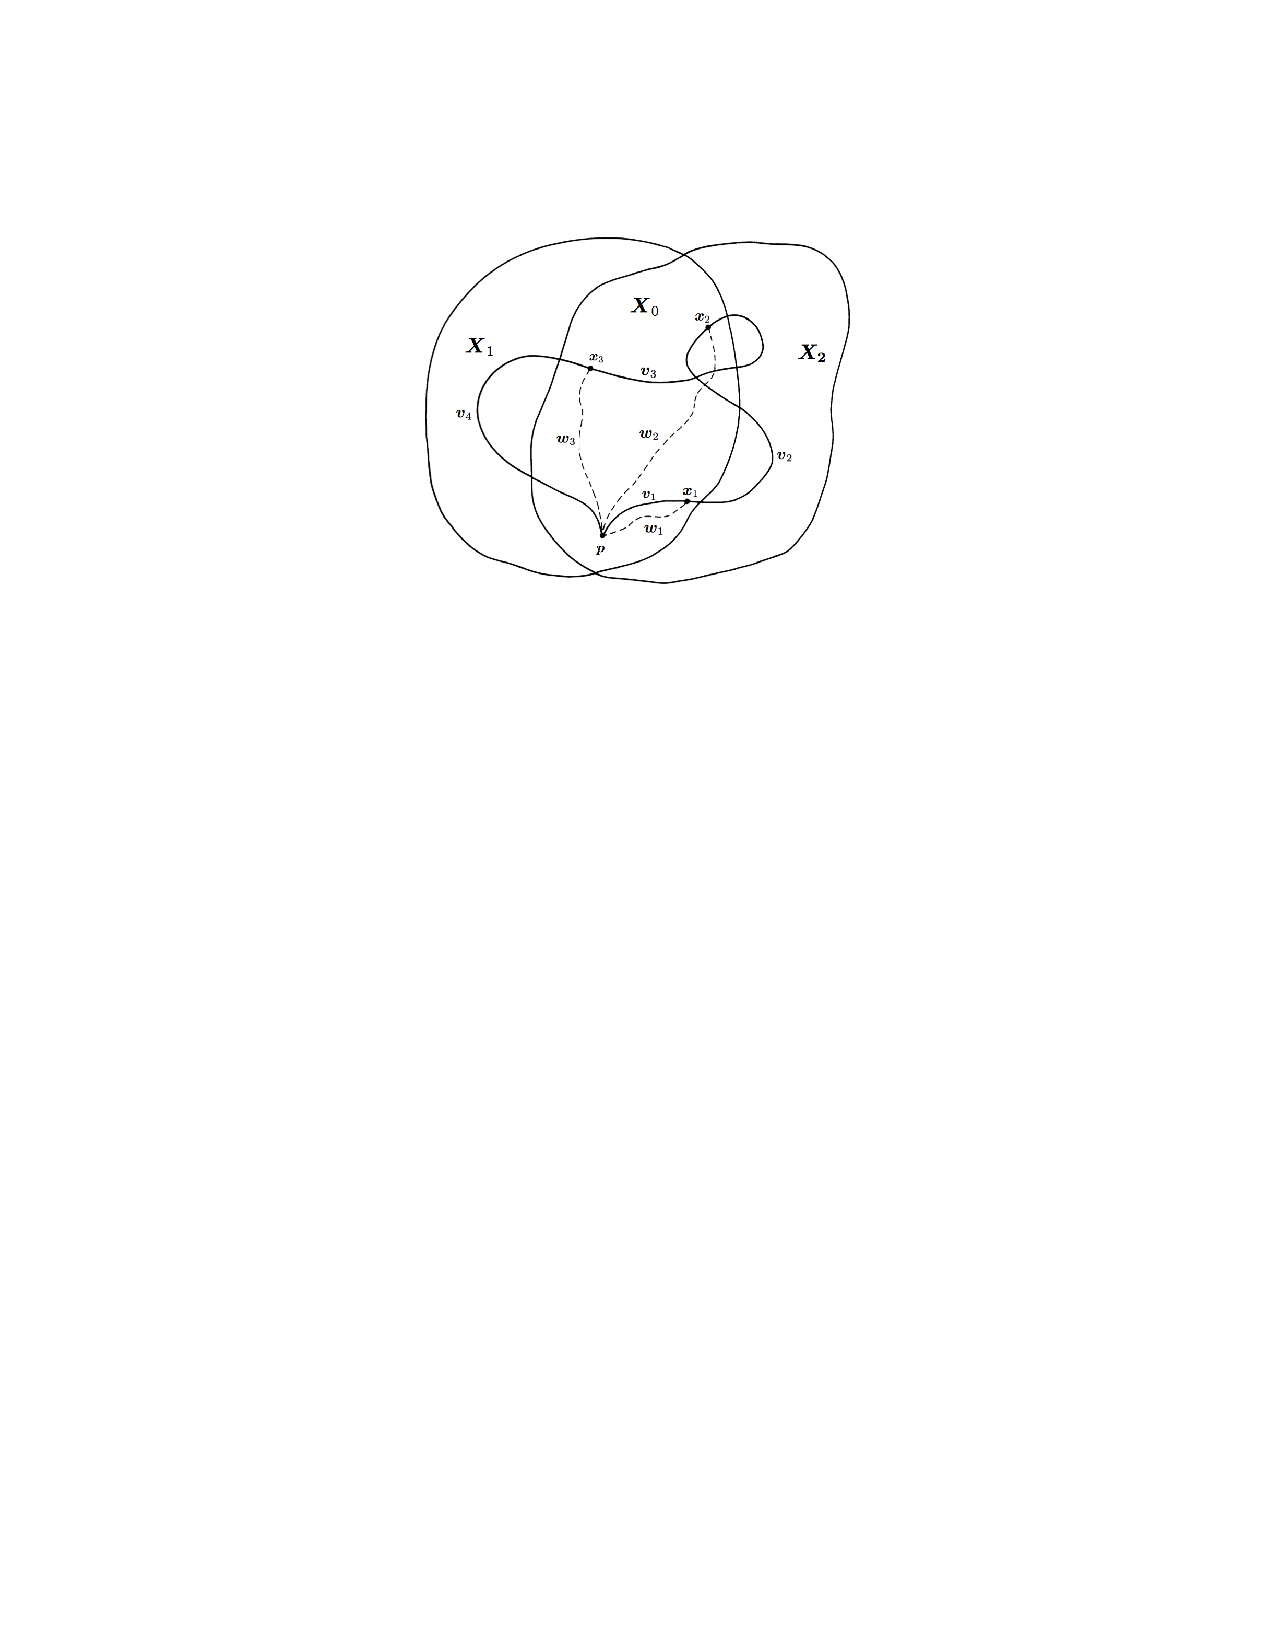
\includegraphics{pictures/vankampen-1.pdf}
\caption{Breaking the path.}
\end{figure}\par
Now we reparametrize $u|_{[x_{i-1},x_i]}$ into a path $v_i:I\to X$: explicitly, let $s_{i-1}<s_i$ be points in $[0,1]$ such that $u(s_{i-1})=x_{i-1}$ and $u(s_i)=x_i$, and define
\[v_i=u\big((1-s)s_{i-1}+ss_i\big)\]
Now, for each $i$, select a path $w_i$ in $X_0$ from $x$ to $x_i$ (take $w_0$ and $w_n$ to be the constant path $c_x$.) Then by concatenating we obtain loops
\[w_{i-1}\ast v_i\ast\widebar{w}_i\]
which lie entirely in either $X_1$ or $X_2$. Each path therefore gives a element in $\pi_1(X_1,x)$ of $\pi_1(X_2,x)$, and we find
\[u\simeq\prod_{i=1}^{n}(w_{i-1}\ast v_i\ast\widebar{w}_i).\]
We can now define $\psi$ by
\[\psi(u):=\phi_*[w_0\ast v_1\ast\widebar{w}_1]\cdot\phi_*[w_1\ast v_2\ast\widebar{w}_2]\cdots\phi_*[w_{n-1}\ast v_n\ast\widebar{w}_n]\]
where $\phi_*$ means either $\phi_1$ or $\phi_2$ depending on the path. If $w_i\ast v_i\ast\widebar{w}_{i}$ lies both in $X_1$ and $X_2$, then it is in fact in $\pi_1(X_0,x)$, and the commutativity of $(\ref{van kam-1})$ tells us that choosing $\phi_1$ or $\phi_2$ does not matter.\par
It is clear that such homomotphism $\psi$ can only be defined in this way, and it is indeed a homomorphism. The commutativity of $(\ref{van kam-2})$ is immediate. What still needs some work is that whether $\psi$ is well defined.\par
First we check that the definition of $\psi$ is independent of the points $x_i$ and the paths $w_i$. Start from the case that we choose a point $x_i$, and $w'_i$ is another path from $x$ to $x_i$.
\[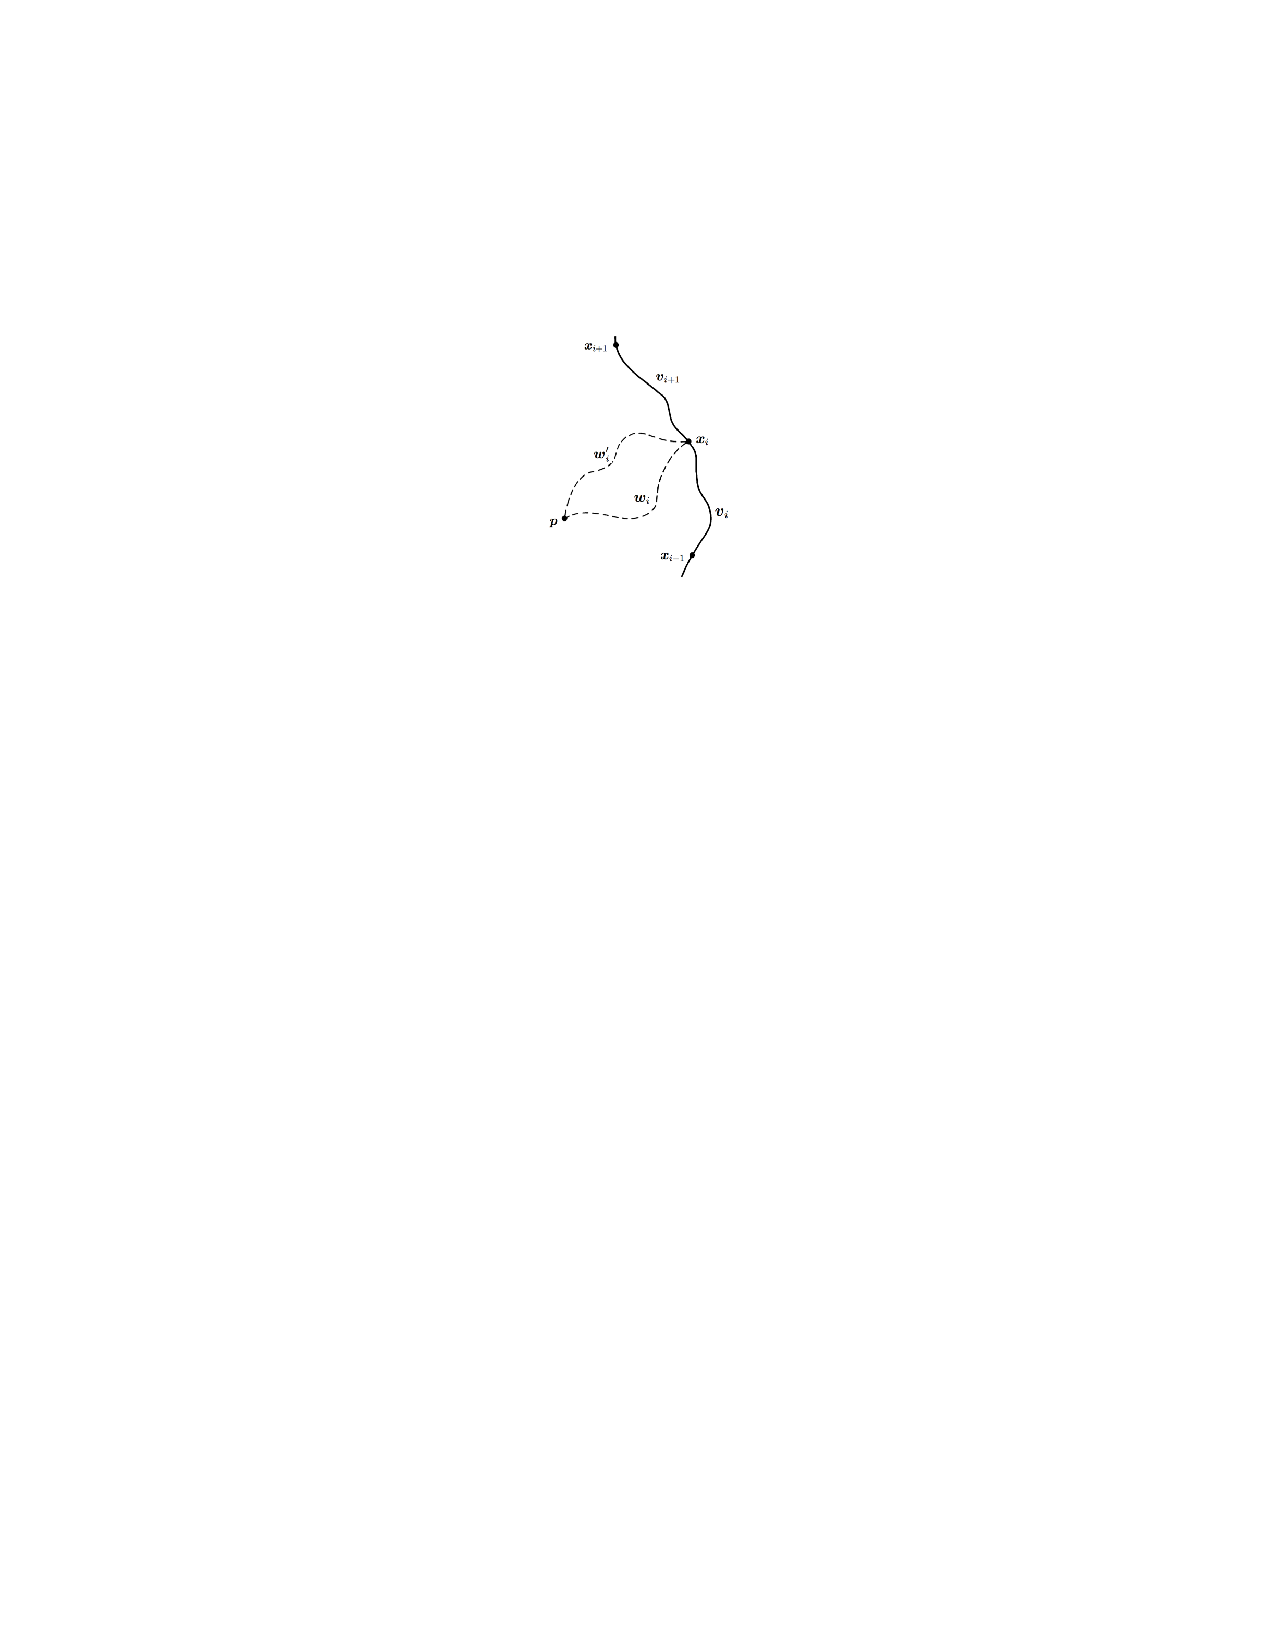
\includegraphics{pictures/vankampen-2.pdf}\]
Then we have
\[\phi_*[w_i\ast v_{i+1}\ast\widebar{w}_{i+1}]=\phi_*[w_i\ast \widebar{w}'_i\ast w'_i\ast v_{i+1}\ast\widebar{w}_{i+1}]=\phi_*[w_i\ast\widebar{w}'_i]\cdot\phi_*[w'_i\ast v_{i+1}\ast\widebar{w}_{i+1}].\]
On the other hand, 
\[\phi_*[w_{i-1}\ast v_i\ast\widebar{w}_i]=\phi_*[w_{i-1}\ast v_i\ast\widebar{w}'_i]\cdot\phi_*[w'_i\ast\widebar{w}_i]=\phi_*[w_{i-1}\ast v_i\ast\widebar{w}'_i]\cdot\big(\phi_*[w_i\ast\widebar{w}'_i]\big)^{-1}.\]
Thus
\[\phi_*[w_{i-1}\ast v_i\ast\widebar{w}_i]\cdot\phi_*[w_i\ast v_{i+1}\ast\widebar{w}_{i+1}]=\phi_*[w_i\ast\widebar{w}'_i]\cdot\phi_*[w_{i-1}\ast v_i\ast\widebar{w}'_i].\]
This gives the independence of the choosen paths $w_i$.\par
Now Suppose another point $y\in X_0$ is added along $v_i$ separating the path $v_i$ into two new paths $v'_i$ and $v'_{i-1}$.
\[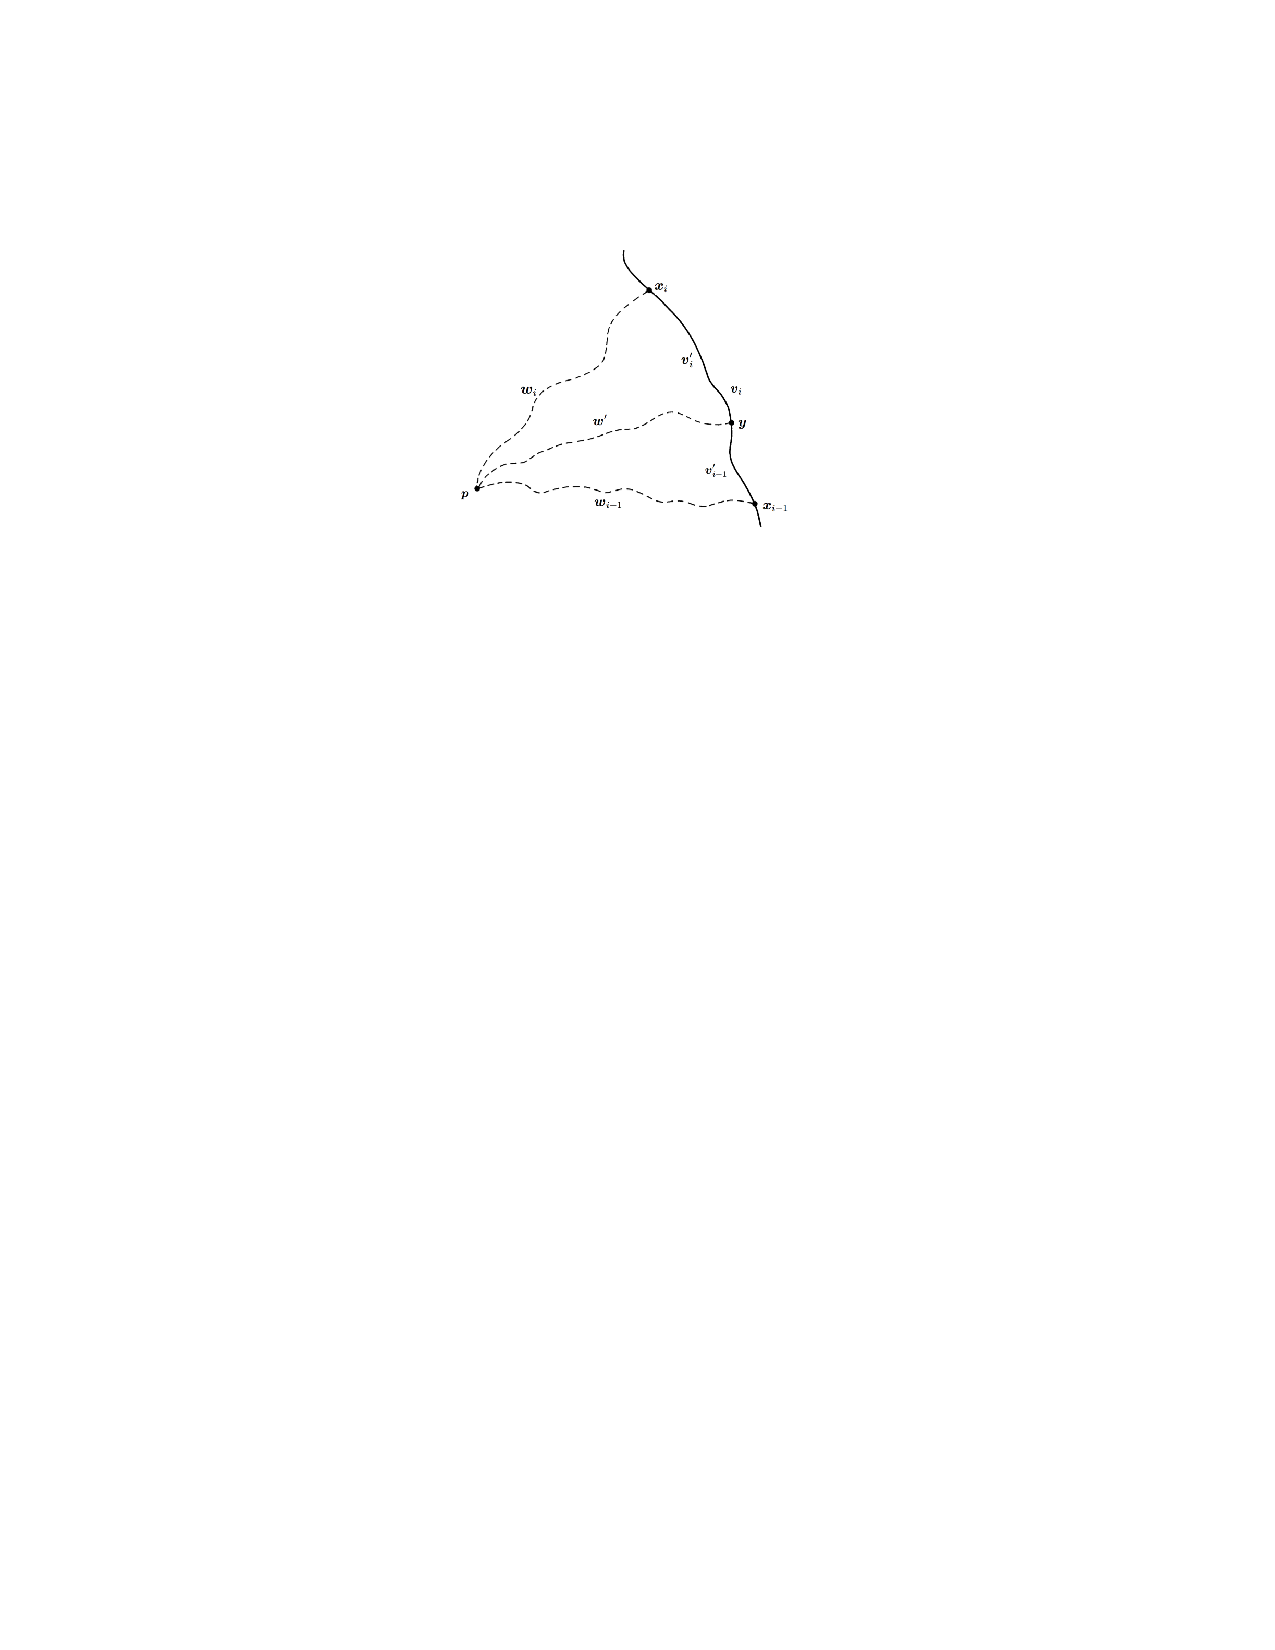
\includegraphics[width=0.3\textwidth]{pictures/vankampen-3.pdf}\]
Choose a path $w'$ from $x$ to $y$ in $X_0$. Suppose for definiteness that the loop $w_{i-1}\ast v_i\ast\widebar{w}_i$ is contained in $X_1$. Then the same is true of the two new loops $w_{i-1}\ast v'_{i-1}\ast\widebar{w}'$ and $w'\ast v'_i\ast\widebar{w}_i$ since $w'_i\sub X_0$, and we have
\[\phi_1[w_{i-1}\ast v'_{i-1}\ast\widebar{w}']\cdot\phi_1[w'\ast v'_i\ast\widebar{w}_i]=\phi_1[w_{i-1}\ast v'_{i-1}\ast\widebar{w}'\ast w'\ast v'_i\ast\widebar{w}_i]=\phi_1[w_{i-1}\ast v_i\ast\widebar{w}_i]\]
This shows that adding an additional point to the set of $\{x_i\}$ does not change the value of $[u]$. More generally, the same is true if we add a finite number of points, that is, refining $\{x_i\}$ leads to the same result. Now suppose we are given two different sets $\{x_i\}$ and $\{y_i\}$ of points. Their union is a common refinement of both $\{x_i\}$ and $\{y_i\}$, and we have just shown that the value of $[u]$ doesn't change when refining the set of points. Thus the value of $[u]$ is the same if we use either the $\{x_i\}$ and $\{y_i\}$.\par
Now we move to the homotopy. Suppose $u$ and $u'$ are two homotopic loops and $U:u\simeq u'$ is a homotopy. We subdivide the square $I\times I$ into lots of
little squares in such a way that each smaller square is mapped by $U$ into either $X_1$ or $X_2$. Such a decomposition exists by Lemma~\ref{Lebesgue lem}, where we take the open cover of $I\times I$ given by the connected components of $U^{-1}(X_1)$ and $U^{-1}(X_2)$. 
\[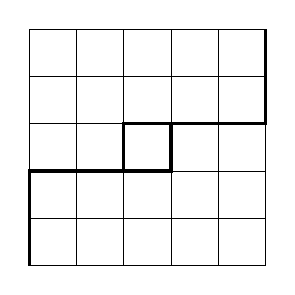
\begin{tikzpicture}[scale=3]
\draw (0,0) rectangle (1,1);
\draw[black,very thick] (0,0) -- (0,0.4)--(0.4,0.4)--(0.4,0.6)--(1,0.6)--(1,1);
\draw[black,very thick] (0.4,0.4)--(0.6,0.4)--(0.6,0.6);
\draw (0.2,0)--(0.2,1) (0.4,0)--(0.4,1) (0.6,0)--(0.6,1) (0.8,0)--(0.8,1);
\draw (0,0.2)--(1,0.2) (0,0.4)--(1,0.4) (0,0.6)--(1,0.6) (0,0.8)--(1,0.8); 
\end{tikzpicture}\]
Proceeding one small rectangle at a time, this deforms $u$ into $u'$ through a finite sequence of paths such that each step involves a homotopy in which the only change occurs within either $X_1$ or $X_2$. For such a restricted deformation, the points $\{x_i\}$ may be chosen so that the value of is unchanged. This completes
the proof.
\end{proof}
\begin{corollary}\label{van kampen coro}
Under the assumptions of Theorem~\ref{van kampen classic}, one has:
\begin{itemize}
\item If $X_2$ is simply connected then 
\[\pi_1(X_1,x)\to\pi_1(X,x)\]
is a surjection with kernel the normal subgroup generated by $\pi_1(i_1)(\pi_1(X,x))$.
\item If $X_0$ is simply connected then $\pi_1(X,x)$ is the free product of $\pi_1(X_1,x)$ and $\pi_1(X_2,x)$.
\item If $X_2$ and $X_0$ are simply connected then
\[\pi_1(X_1,x)\to\pi_1(X,x)\]
is an isomorphism.
\end{itemize}
\end{corollary}
\subsection{Graphs}
A graph is a CW complex of dimension $0$ or $1$. The $0$-cells of a graph are called its \textbf{vertices}, and the $1$-cells are called its edges. It follows from the definition of a CW complex that for each edge $e$, the set $\widebar{e}\setminus e$ consists of one or two vertices; if a vertex $v$ is contained in $\widebar{e}$, we say that $v$ and $e$ are \textbf{incident}. A \textbf{subgraph} is a subcomplex of a graph; thus if a subgraph contains an edge, it also contains the vertex or vertices incident with it.\par
An edge that is incident with only one vertex is called a \textbf{self-loop}. If two or more edges are incident with the same one or two vertices, they are called \textbf{multiple edges}. A graph with no self-loops or multiple edges is called a \textbf{simple graph}. (Some graph theory texts reserve the term graph to refer to a simple graph, in which case the more general kind of graph defined here is usually called a multigraph.)\par
An \textbf{edge path} in a graph is a finite sequence $(v_0,e_1,v_1,\cdots,v_{k-1},e_k,v_k)$ that starts and ends with vertices and alternates between vertices and edges, such that for each $i$, $\{v_{i-1},v_i\}$ is the set of vertices incident with the edge $e_i$. (Thus $v_{i-1}=v_i$ if and only if $e_i$ is a self-loop.) The vertices $v_0$ and $v_k$ are called the \textbf{initial vertex} and \textbf{terminal vertex} of the edge path, respectively, and we say it is an edge path from $v_0$ to $v_k$. We also allow a \textbf{trivial edge path} $(v_0)$ consisting of one vertex alone. An edge path is said to be \textbf{closed} if $v_0=v_k$, and \textbf{simple} if no edge or vertex appears more than once, except that $v_0$ might be equal to $v_k$.\par
A \textbf{cycle} is a nontrivial simple closed edge path. A \textbf{tree} is a connected graph that contains no cycles. A tree cannot contain self-loops or multiple edges: if $e$ is a self-loop incident with the vertex $v$, then $(v,e,v)$ is a cycle; and if $e'$ and $e''$ are two edges incident with the vertices $v'$ and $v''$, then $(v',e',v'',e'',v')$ is a cycle. It follows that every tree is a simple graph.
\begin{figure}[htpb]
\centering
\begin{minipage}{200pt}
\centering
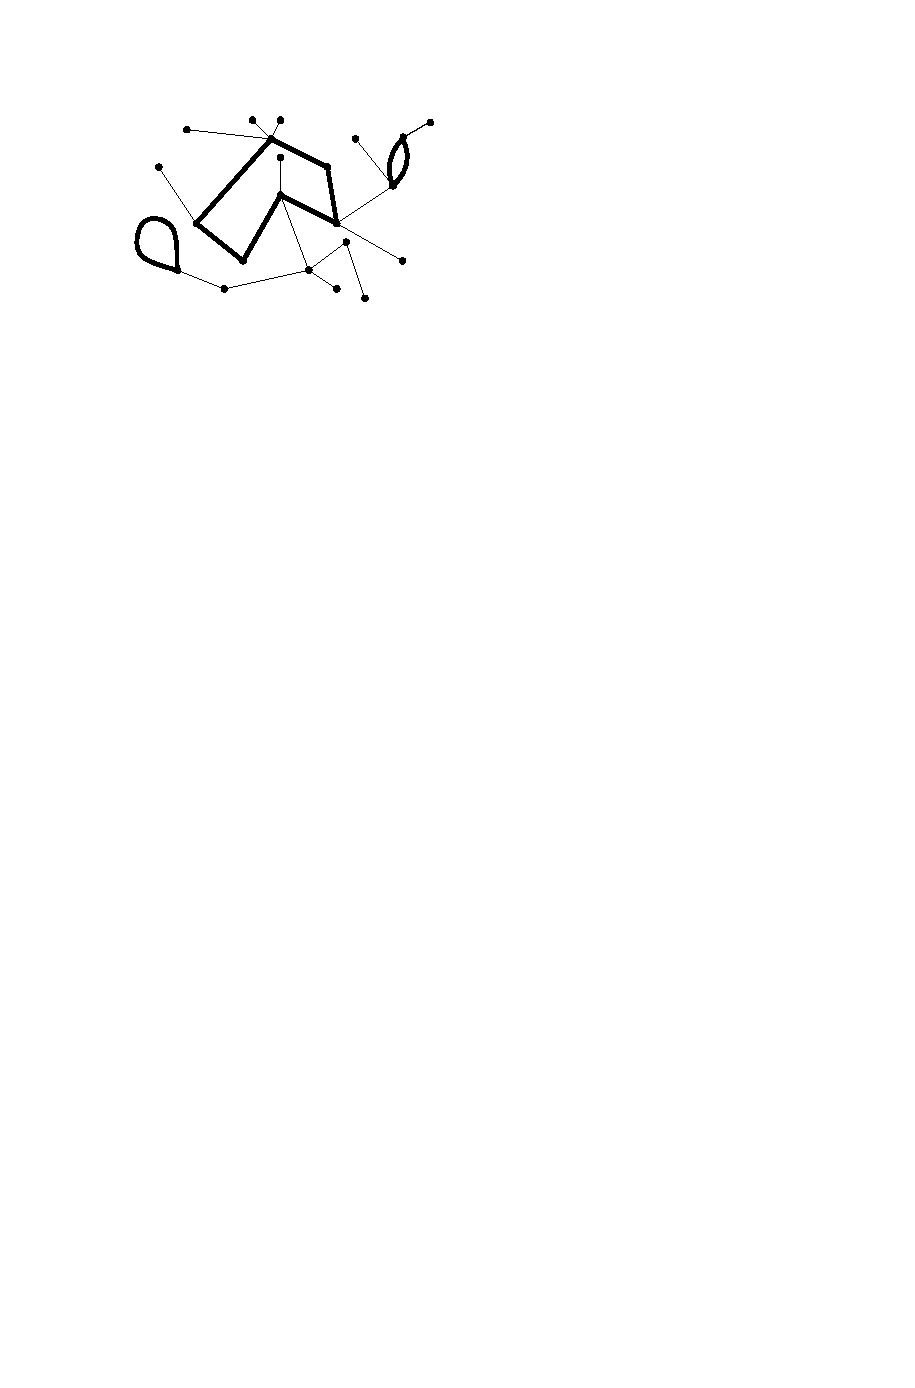
\includegraphics{pictures/Graph-eg1}
\caption{A graph with three cycles.}
\end{minipage}
\hspace{20pt}
\begin{minipage}{200pt}
\centering
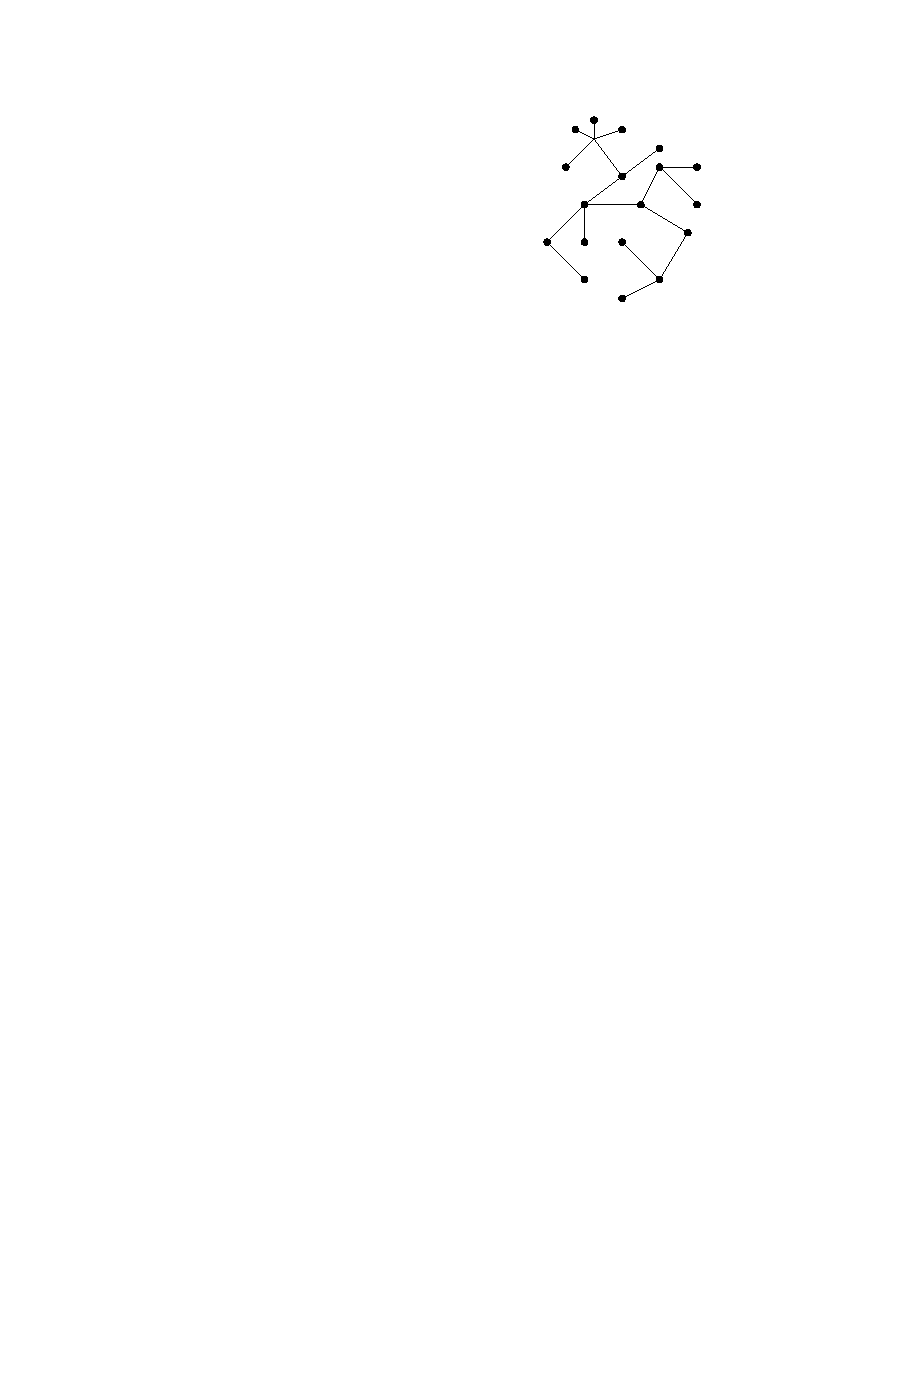
\includegraphics{pictures/Graph-eg2}
\caption{A tree.}
\end{minipage}
\end{figure}
\begin{proposition}\label{tree contractible}
Every finite tree is contractible, and thus simply connected.
\end{proposition}
\begin{proof}
Let $T$ be a finite tree. The proof is by induction on the number of edges in $T$. If there are no edges, then $T$ consists of a single vertex and is therefore contractible.
So assume every tree with $n$ edges is contractible, and let $T$ be a tree with $n+1$
edges.\par
Because $T$ is a simple graph, every edge of $T$ is incident with exactly two vertices.
If every vertex in $T$ is incident with at least two edges, then arguing exactly as in the proof of the classification theorem for $1$-manifolds, we can construct doubly infinite sequences $(v_j)_{j\in\Z}$ of vertices and $(e_j)_{j\in\Z}$ of edges such that for each $j$, $v_{j-1}$ and $v_j$ are the two vertices incident with $e_j$, and $e_j$, $e_{j+1}$ are two different edges incident with $v_j$. Because $T$ is finite, there must be some integers $n$ and $n+k>n$ such that $v_n=v_{n+k}$. If $n$ and $k$ are chosen so that $k$ is the minimum positive integer with this property, this means that $(v_n,e_{n+1},\cdots,e_{n+k},v_{n+k})$ is a cycle, contradicting the assumption that $T$ is a tree. Thus there must be a vertex $v$ that is incident with at most one edge. Since $T$ is connected, $v$ is incident with exactly one edge, say $e$, and $e$ is incident with exactly one other vertex $v'$.\par 
Let $T'$ be the subgraph of $T$ with the vertex $v$ and the edge $e$ deleted. The constant map from $\widebar{e}$ onto $\{v'\}$ is a strong deformation retraction; extending this to be the identity on $T'$ yields a strong deformation retraction of $T$ onto $T'$. Therefore, $T$ is homotopy equivalent to $T'$, which is contractible by the induction hypothesis.
\end{proof}
Let $\Gamma$ be a graph. A \textbf{spanning tree} in $\Gamma$ is a subgraph that is a tree and that contains every vertex of $\Gamma$.
\begin{proposition}
Every finite connected graph contains a spanning tree.
\end{proposition}
\begin{proof}
Let $\Gamma$ be a finite connected graph. If $\Gamma=\emp$, then the empty subgraph is
a spanning tree. Otherwise, we begin by showing that $\Gamma$ contains a \textbf{maximal tree}, meaning a subgraph that is a tree and is not properly contained in any larger tree in $\Gamma$. To prove this, start with any nonempty tree $T_0\sub\Gamma$ (e.g., a single vertex). If it is not maximal, then it is contained in a strictly larger tree $T_1$. Continuing in this way by induction, we obtain a sequence of trees $T_0\sub T_1\sub\cdots$, each properly contained in the next. Because $\Gamma$ is finite, the process cannot go on forever, so eventually we obtain a tree $T\sub\Gamma$ that is not contained in any strictly larger tree.\par
To show that $T$ is a spanning tree, suppose for the sake of contradiction that there
is a vertex $v\in\Gamma$ that is not contained in $T$. Because $\Gamma$ is connected, there is an edge path from a vertex $v_0\in T$ to $v$, say $(v_0,e_1,\cdots,e_k,v_k=v)$. Let $v_i$ be the last vertex in the edge path that is contained in $T$. Then the edge $e_{i+1}$ is not contained in $T$, because if it were, $v_{i+1}$ would also be in $T$ because $T$ is a subgraph. The subgraph $T'=T\cup\widebar{e}_{i+1}$ properly contains $T$, so it is not a tree, and therefore contains a cycle. This cycle must include $e_{i+1}$ or $v_{i+1}$, because otherwise it would be a cycle in $T$. However, since $e_{i+1}$ is the only edge of $T'$ that is incident with $v_{i+1}$, there can be no such cycle.
\end{proof}
Let $\Gamma$ be a finite connected graph. We construct a set of generators for the fundamental group of $\Gamma$ as follows. Choose a vertex $v$ as base point, and let $T\sub\Gamma$ be a spanning tree. Let $e_1,\cdots,e_n$ be the edges of $\Gamma$ that are not in $T$, and for each $i$ let $\{w_i,w'_i\}$ be the set of vertices incident with $e_i$. (Thus $w_i=w'_i$ if $e_i$ is a self-loop.) We can choose paths $g_i$ and $h_i$ in $T$ from $v$ to $w_i$ and $w'_i$, respectively. Let $f_i$ denote the loop in $\Gamma$ obtained by first following $g_i$ from $v$ to $w_i$, then traversing $e_i$, and then following $\bar{h}_i$ from $w'_i$ back to $v$. Note that the path class is independent of the choices of $g_i$ and $h_i$, because any two paths in $T$ with the
same endpoints are path-homotopic.
\begin{figure}[htbp]
\centering
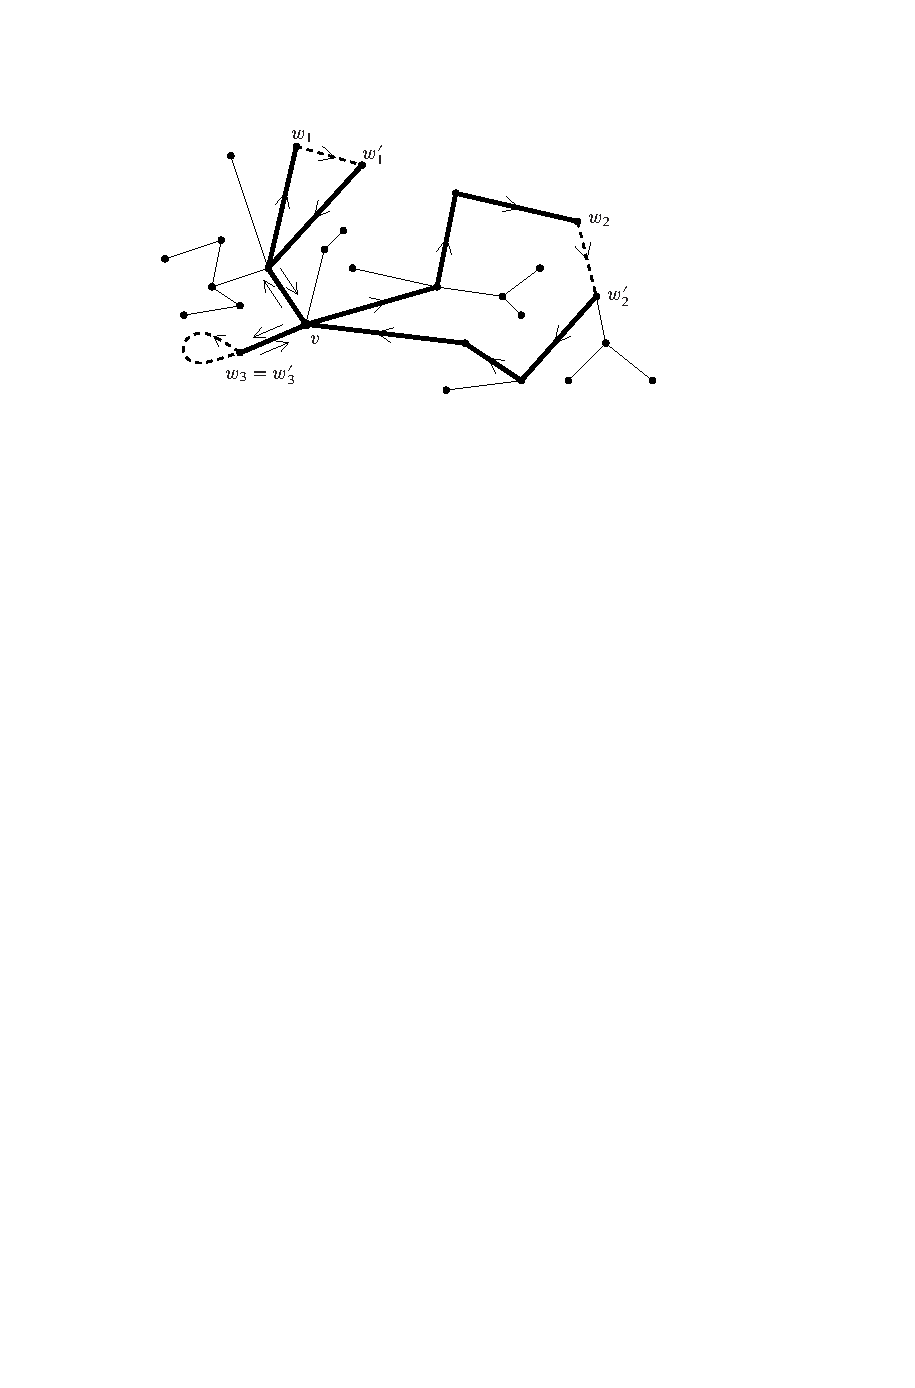
\includegraphics{pictures/fandamental-graph-1}
\caption{Generators for the fundamental group of a graph.}
\end{figure}
\begin{theorem}[Fundamental Group of a Finite Graph]\label{fund graph}
The fundamental group of a finite connected graph $\Gamma$ based at a vertex $v$ is the free group on the path classes $[f_1],\cdots,[f_n]$ constructed above.
\end{theorem}
\begin{proof}
We prove the theorem by induction on the number $n$ of edges in $\Gamma\setminus T$. If $n=0$, then $\Gamma$ is a tree and hence simply connected, so there is nothing 
to prove.\par
For $n=1$, we must show that $\Gamma$ is the infinite cyclic group generated by $[f_1]$. Let $T$ be the chosen spanning tree, and let $e$ be the single edge in 
$\Gamma\setminus T$. By assumption, there is a cycle $(v_0,e_1,\cdots,e_m,v_m)$ in $\Gamma$. This cycle must include the edge $e$, because otherwise it would be a 
cycle in $T$. The subgraph $C\sub\Gamma$ consisting of the union of the vertices and edges $\{v_0,e_1,\cdots,e_m,v_m\}$ is homeomorphic to $S^1$ by the same argument 
as in the proof of Theorem~\ref{class one mani}. We will show that inclusion $C\hookrightarrow\Gamma$ is a homotopy equivalence.\par
Let $K$ be the union of all the edges in $\Gamma\setminus C$ together with their vertices. Each component $K_i$ of $K$ is a connected subgraph of $\Gamma$ contained in $T$, and is therefore a tree (since a cycle in $K_i$ would also be one in $T$). Moreover, each such component shares at least one vertex $y_i$ with $C$ because $\Gamma$ is connected. In fact, it shares exactly one: if $K_i\cap C$ contained two vertices $y_i,y'_i$, it would be possible to find a cycle in $T$ by following an edge path in $K_i$ from $y_i$ to $y'_i$ followed by the edge path in $C$ from $y'_i$ to $y_i$ that does not contain $e$. (This is possible since $C\approx S^1$.)\par
Now define a strong deformation retraction of $\Gamma$ onto $C$ as follows: on each $K_i$, it is a strong deformation retraction of $K_i$ onto $y_i$, which exists since $K_i$ is contractible; and on $C$ it is the identity. The resulting map is continuous by the gluing lemma, and shows that $\Gamma\simeq S^1$.\par
It remains to show that the path class $[f_1]$ is a generator of $\pi_1(\Gamma,v)$. Let $z$ be any vertex in $C$. A path $a$ that starts at $z$ and traverses each edge of $C$ in order is clearly path-homotopic to the standard generator of $S^1\approx C$ (or its inverse). Choosing any path $b$ from $z$ to $v$ yields an isomorphism $\varPhi_b:\pi_1(\Gamma,z)\to\pi_1(\Gamma,v)$. Thus a generator of $\pi_1(\Gamma,v)$ is $\varPhi_b[a]=[\bar{b}\ast a\ast b]$. Since $\bar{b}\ast a\ast b$ is a path that
goes from $v$ to $w_1$, traverses e, and returns to $v$, it is homotopic to $f_1$. (Remember that the path class of $f_1$ is independent of which paths we choose from $v$ to $w_1$ and $w'_1$ .) This completes the proof in the case $n=1$.\par
Now let $n\geq1$, and assume the conclusion holds for every graph with $n$ edges in
the complement of a spanning tree. Let $\Gamma$ be a graph with a spanning tree $T\sub\Gamma$ such that $\Gamma\setminus T$ consists of $n+1$ edges $e_1,\cdots,e_{n+1}$. We apply the Seifert–Van Kampen theorem in the following way. For each $i=1,\cdots,n+1$, choose a point $x_i\in e_i$. Let $U=\Gamma\setminus\{x_1,\cdots,x_n\}$ and $V=\Gamma\setminus\{x_{n+1}\}$. Both $U$ and
$V$ are open in $\Gamma$, and just as before it is easy to construct deformation retractions to show that $U\cap V\simeq T$, $U\simeq T\cup e_{n+1}$ and $V\simeq\Gamma\setminus e_{n+1}$. By the inductive hypothesis, $\pi_1(V,v)=F([f_1],\cdots,[f_n])$ and $\pi_1(U,v)=F([f_{n+1}])$. Since $U\cap V$ is simply connected, Corollary~\ref{van kampen coro} shows that $\pi_1(\Gamma,v)$ is isomorphic to the free product of these two free groups, which in turn is isomorphic the free group on $F([f_1],\cdots,[f_{n+1}])$ as claimed.
\begin{figure}[htbp]
\centering
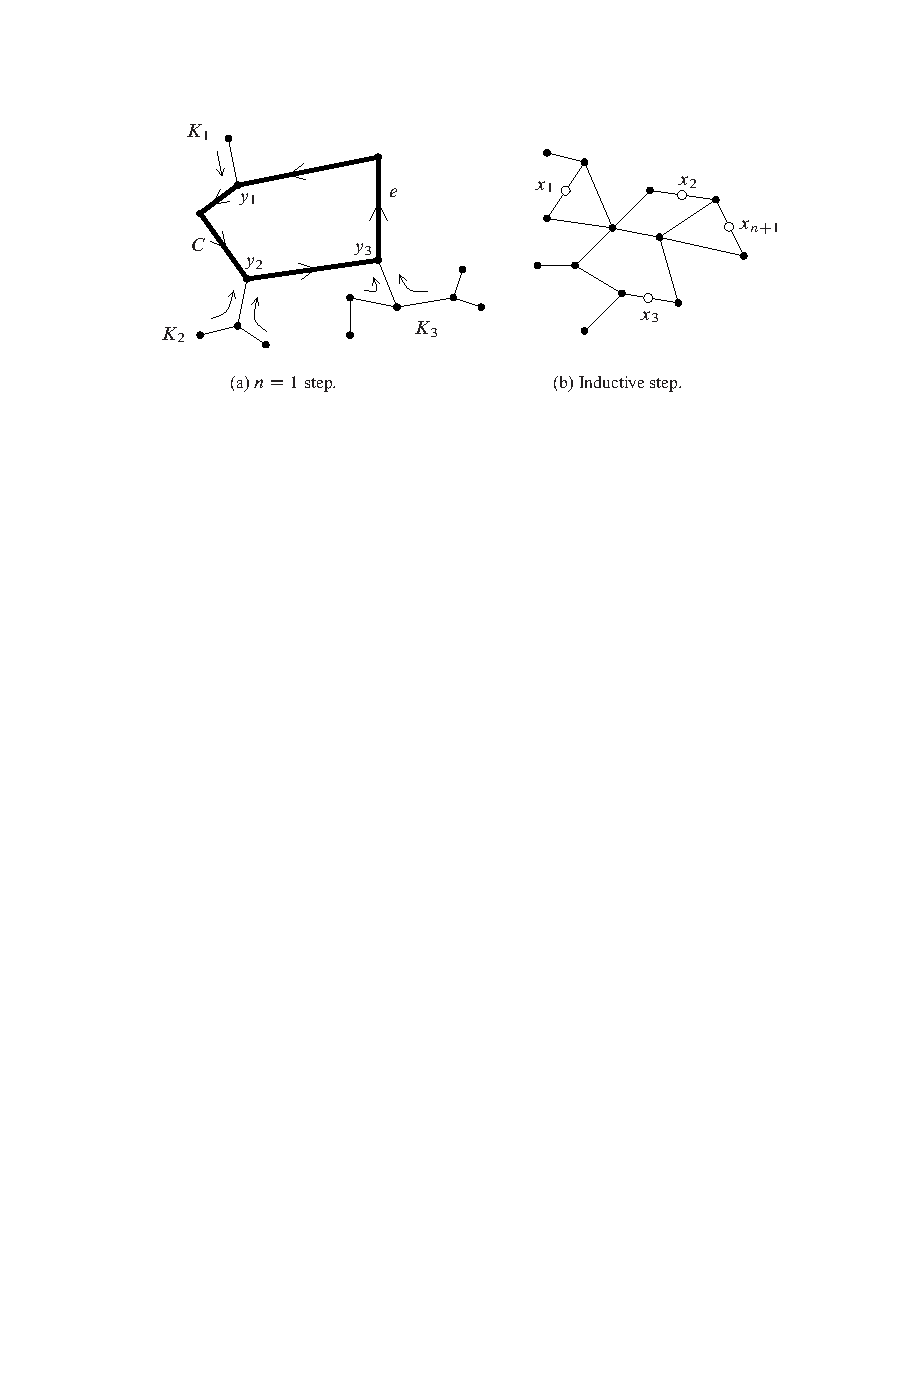
\includegraphics{pictures/fandamental-graph-2}
\end{figure}
\end{proof}
\subsection{Fundamental Groups of CW Complexes}
Our next application of the Seifert–Van Kampen theorem is to give an algorithm for computing a presentation of the fundamental group of a finite CW complex.We have already taken care of the case of a complex of dimension $0$ or $1$ in our treatment
of graphs above. The next step is to examine the consequence of attaching cells of
higher dimensions.\par
We begin with $2$-cells. Although the details of the proof are a bit involved, the basic idea is that when a $2$-cell is attached to a space $X$, the attaching map can be thought of as the circle representative for an element of $\pi_1(X)$, and attaching the cell kills that element because it becomes null-homotopic in the adjunction space.
\begin{proposition}[\textbf{Attaching a Disk}]\label{attaching disk}
Let $X$ be a path-connected topological space, and let $\widetilde{X}$ be the space obtained by attaching a closed $2$-cell $D$ to $X$ along an attaching map $\varphi:\partial D\to X$. Let $v\in\partial D$, $\widetilde{v}=\varphi(v)\in X$ and $\gamma=\varphi_*(\alpha)\in\pi_1(X,\widetilde{v})$, where $\alpha$ is a generator of the infinite cyclic group $\pi_1(\partial D,v)$ Then the homomorphism $\pi_1(X,\widetilde{X})\to\pi_1(\widetilde{X},\widetilde{v})$ induced by inclusion $X\hookrightarrow\widetilde{X}$ is surjective, and its kernel is the smallest normal subgroup containing $\gamma$. If $\pi_1(X,\widetilde{v})$ has a finite presentation
\[\pi_1(X,\widetilde{v})=\langle\beta_1,\cdots,\beta_n\mid\sigma_1,\cdots,\sigma_s\rangle.\]
then $\pi_1(\widetilde{X},\widetilde{v})$ has the presentation
\[\pi_1(\widetilde{X},\widetilde{v})=\langle\beta_1,\cdots,\beta_n\mid\sigma_1,\cdots,\sigma_s,\tau\rangle.\]
where $\tau$ is an expression for $\gamma\in\pi_1(X,\widetilde{v})$ in terms of $\{\beta_1,\cdots,\beta_n\}$.
\end{proposition}
\begin{figure}[htbp]
\centering
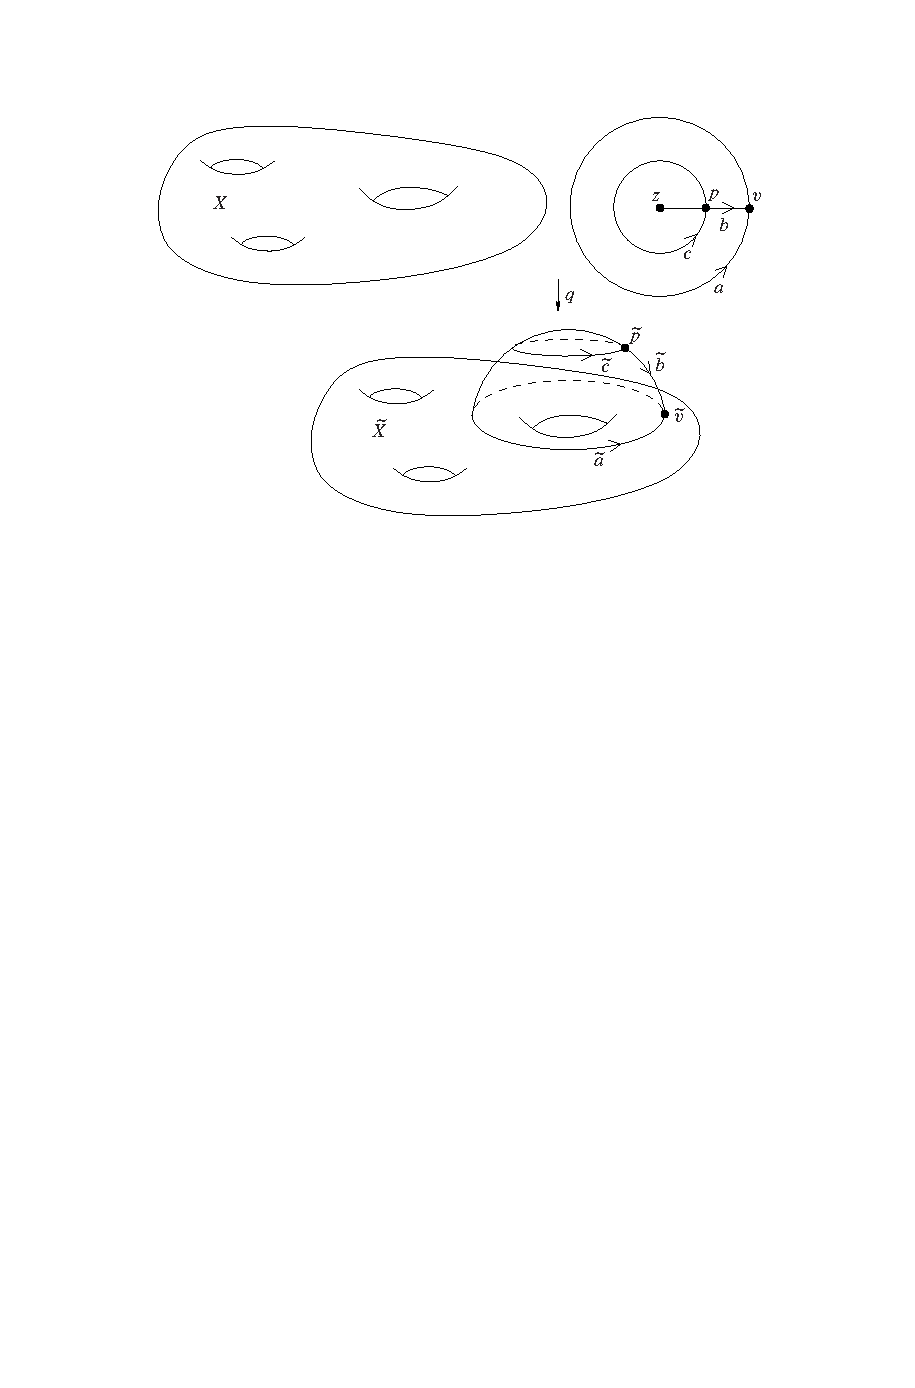
\includegraphics{pictures/attaching-disk}
\caption{Attaching a disk.}
\end{figure}
\begin{proof}
Let $q:X\amalg D\to\widetilde{X}$ be the quotient map. As usual, we identify $X$ with
its image under $q$, so we can consider $X$ as a subspace of $\widetilde{X}$. First we set up some notation. Choose a point $z\in\Int D$, set $U=\Int D$ and $V=X\amalg(D\setminus\{z\})$, and let $\widetilde{U}=q(U)$, $\widetilde{V}=q(V)\sub\widetilde{X}$. Since $U$ and $V$ are saturated open subsets,
the restrictions of $q$ to $U$ and $V$ are quotient maps, and their images $\widetilde{U},\widetilde{V}$ are open in $\widetilde{X}$. Moreover, $\widetilde{U}$ and $\widetilde{U}\cap\widetilde{V}$ are path-connected because they are continuous images of path-connected sets, and $\widetilde{V}$ is path-connected because it is the union of the pathconnected sets $X$ and $\widetilde{U}\cap\widetilde{V}$ that have the point $\widetilde{v}$ in common.\par
In order to apply the Seifert-Van Kampen theorem in this situation, we need to work with a base point in $\widetilde{U}\cap\widetilde{V}$. Choose $p\in\Int D\setminus\{z\}\approx\B^2\setminus\{0\}$, and let $c:I\to\Int D\setminus\{z\}$ be a loop based at $p$ whose path class generates $\pi_1(\Int D\setminus\{z\},p)$. Then
let $\widetilde{p}=q(p)\in\widetilde{U}\cap\widetilde{V}$, and $\widetilde{c}=q\circ c$. In general, we use symbols without tildes to denote sets, points, or paths in $D$, and the same symbols with tildes to denote their images in $\widetilde{X}$.\par
The restriction of $q$ to $U$ is a one-to-one quotient map and therefore a homeomorphism onto its image. Since $U$ is simply connected, so is $\widetilde{U}$. On the other hand, $\widetilde{U}\cap\widetilde{V}$ is the image under $q$ of the saturated open subset $\Int D\setminus\{z\}$, so $q:\Int D\setminus\{z\}\to\widetilde{U}\cap\widetilde{V}$ is an injective quotient map and thus a homeomorphism. It follows that $\pi_1(\widetilde{U}\cap\widetilde{V},\widetilde{p})$ is the infinite cyclic group generated by $[\widetilde{c}]$. Now Corollary~\ref{van kampen coro} implies that inclusion $\widetilde{V}\hookrightarrow\widetilde{X}$ induces a surjective map
\begin{align}\label{attaching idsk-1}
\pi_1(\widetilde{V},\widetilde{p})\to\pi_1(\widetilde{X},\widetilde{p}).
\end{align}
whose kernel is the normal closure of the cyclic subgroup generated by $[\widetilde{c}]$.\par
To complete the proof, we just need to relate the fundamental group of $\widetilde{V}$ with that of $X$. Combining a strong deformation retraction of $D\setminus\{z\}$ onto $\partial D$ with the identity map of $X$, we obtain a homotopy $H:V\times I\to V$ that yields a strong deformation retraction of $V$ onto $X\amalg\partial D$. Because $q\circ H$ respects the identifications made by $q\times id_I:V\times I\to\widetilde{V}\times I$, it descends to a strong deformation retraction of $\widetilde{V}$ onto $X$. Therefore the inclusion $X\hookrightarrow\widetilde{V}$ is a homotopy equivalence. Thus we can replace $\pi_1(\widetilde{V},\widetilde{v})$ with $\pi_1(X,\widetilde{v})$ in $(\ref{attaching idsk-1})$, and we still have a surjective homomorphism whose kernel is the smallest normal subgroup containing $\gamma$. The statement about presentations then follows from the definition of push out.
\end{proof}
The analogous result for higher-dimensional cells is much simpler.
\begin{proposition}[\textbf{Attaching an $\bm{n}$-cell}]\label{attaching n cell}
Let $X$ be a path-connected topological space, and let $\widetilde{X}$ be a space obtained by attaching an $n$-cell to $X$, with $n\geq3$. Then inclusion $X\hookrightarrow\widetilde{X}$ induces an isomorphism of fundamental groups.
\end{proposition}
\begin{proof}
We define open subsets $\widetilde{U},\widetilde{U}\cap\widetilde{V}$ just as in the preceding proof. In this case, $\widetilde{U}\cap\widetilde{V}$ is simply connected, because it is homeomorphic to $\B^n\setminus\{0\}$, and the result follows.
\end{proof}
Putting these results together, we obtain the following powerful theorem. For technical reasons, the computations are much simpler if we assume that the base point lies in the closure of each of the $2$-cells.
\begin{theorem}
Suppose $X$ is a connected finite CW complex, and $v$ is a point in the $1$-skeleton of $X$ that is contained in the closure of every $2$-cell. Let $\beta_1,\cdots,\beta_n$ be generators for the free group $\pi_1(X_1,v)$ $($$X_1$ is a graph$)$, and let $e_1,\cdots,e_k$ be the $2$-cells of $X$. For each $i=1,\cdots,k$, let $\Phi_i:D_i\to X$ be a characteristic map for $e_i$ that takes $v_i\in\partial D_i$ to $v$, let $\varphi_i=\Phi_i|_{\partial D_i}:\partial D_i\to X_1$ be the corresponding attaching map, let $\alpha_i$ be a generator of $\pi_1(\partial_i,v_i)$, and let $\sigma_i$ be an expression for $(\varphi_i)_*(\alpha_i)\in\pi_1(X,v)$ in terms of the generators $\{\beta_i\}$. Then $\pi_1(X,v)$ has the following presentation:
\[\pi_1(X,v)=\langle\beta_1,\cdots,\beta_n\mid\sigma_1,\cdots,\sigma_k\rangle\]
\end{theorem}
\begin{proof}
This follows immediately by induction from the two preceding propositions,
using the result of Exercise~\ref{CW minus n-cell}.
\end{proof}
\subsection{Fundamental Groups of Compact Surfaces}
The computations in this chapter allow us to compute the fundamental groups of all compact surfaces. Now it will become clear why we chose similar notations for surface presentations and group presentations.
\begin{theorem}
Let $M$ be a topological space with a polygonal presentation $\langle a_1,\cdots,a_n\mid W\rangle$ with one face, in which all vertices are identified to a single point. Then $\pi_1(M)$ has the presentation $\langle a_1,\cdots,a_n\mid W\rangle$.
\end{theorem}
\begin{proof}
As we have observed, a polygonal presentation determines a CW decomposition of $M$ in a natural way. Under the assumption that all the vertices are identified to a single point, the $1$-skeleton $M_1$ is a wedge sum of circles, one for each symbol in the presentation, and thus its fundamental group has the presentation $\langle a_1,\cdots,a_n\mid\emp\rangle$. The attaching map of the single $2$-cell maps the boundary of the polygon onto the loop in $M_1$ obtained by following the generators in the order specified by the word $W$. The result follows immediately from Proposition~\ref{attaching disk}.
\end{proof}
\begin{corollary}[\textbf{Fundamental Groups of Compact Surfaces}]
The fundamental groups of compact connected surfaces have the following presentations:
\begin{itemize}
\item[$(a)$] $\pi_1(S^2)=\langle\emp\mid\emp\rangle$ $($the trivial group$)$.
\item[$(b)$] $\pi_1(T^2\#\cdots\#T^2)=\langle\beta_1,\gamma_1,\cdots,\beta_n,\gamma_n\mid\beta_1\gamma_1\beta_1^{-1}\gamma_1^{-1}\cdots\beta_n\gamma_n\beta_n^{-1}\gamma_n^{-1}=1\rangle$.
\item[$(c)$] $\pi_1(\P^2\#\cdots\#\P^2)=\langle\beta_1,\cdots,\beta_n\mid\beta_1^2\cdots\beta_n^2=1\rangle$.
\end{itemize}
\end{corollary}
In particular, for the torus this gives $\pi_1(T^2)=\langle\beta,\gamma\mid\beta\gamma=\gamma\beta\rangle=\Z^2$, which agrees with the result we derived earlier. In the case of the projective plane, this gives $\pi_1(\P^2)=\langle\beta\mid\beta^2=1\rangle=\Z/2\Z$.\par
The quotient group $G/[G,G]$ is denoted by $Ab(G)$ and called the \textbf{abelianization} of $G$. Because an isomorphism $F:G_1\to G_2$ takes the commutator subgroup of $G_1$ to that of $G_2$, isomorphic groups have isomorphic abelianizations. The abelianization is the largest abelian quotient of $G$, or equivalently the largest abelian homomorphic image of $G$, in the sense that any other homomorphism into an abelian group factors through the abelianization.
\begin{proposition}
The fundamental groups of compact surfaces have the following abelianizations:
\begin{itemize}
\item[$(a)$] $Ab\big(\pi_1(S^2)\big)=\{0\}$.
\item[$(b)$] $Ab\big(\pi_1(\underbrace{T^2\#\cdots\#T^2}_{n})\big)=\Z^{2n}$.
\item[$(c)$] $Ab\big(\pi_1(\underbrace{\P^2\#\cdots\#\P^2}_{n})\big)=\Z^{n-1}\times\Z/2\Z$.
\end{itemize}
\end{proposition}
\begin{proof}
The case of the sphere is immediate. Consider next an orientable surface of genus $n$, and let
\[G=\langle\beta_1,\gamma_1,\cdots,\beta_n,\gamma_n\mid\beta_1\gamma_1\beta_1^{-1}\gamma_1^{-1}\cdots\beta_n\gamma_n\beta_n^{-1}\gamma_n^{-1}=1\rangle\]
be the fundamental group. Define a map $\varphi:G\to\Z^{2n}$ as follows. Let $e_i=(0,\cdots,1,\cdots,0)\in\Z^{2n}$ ($1$ in the $i$-th place), and set
\[\varphi(\beta_i)=e_i,\quad\varphi(\gamma_i)=e_{i+n}.\]
As a map from the free group $F(\beta_1,\gamma_1,\cdots,\beta_n,\gamma_n)$ into $\Z^{2n}$, this sends the element $\beta_1\gamma_1\beta_1^{-1}\gamma_1^{-1}\cdots\beta_n\gamma_n\beta_n^{-1}\gamma_n^{-1}$ to $(0,\cdots,0)$, so it descends to a homomorphism from $G$ to $\Z^{2n}$. By the characteristic property of the abelianization, it also descends to a homomorphism (still denoted by $\varphi$) from $Ab(G)$ to $\Z^{2n}$.\par
To go back the other way, define $\psi:\Z^{2n}\to Ab(G)$ by
\[\psi(e_i)=\begin{cases}
[\beta_i],&1\leq i\leq n;\\
[\gamma_{i-n}],&n+1\leq i\leq 2n.
\end{cases}\]
where the brackets on the right-hand side denote the equivalence class in $Ab(G)$,
and extend it to be a homomorphism. It is easy to check that $\psi$ and $\varphi$ are inverses of each other.\par
Next consider a connected sum of projective planes, and write the fundamental group as
\[H=\langle\beta_1,\cdots,\beta_n\mid\beta_1^2\cdots\beta_n^2=1\rangle.\]
Let $f$ denote the nontrivial element of $\Z/2\Z$, and define $\varphi:Ab(H)\to\Z^{n-1}\times\Z/2\Z$ by
\[\varphi(\beta_i)=\begin{cases}
e_i,&1\leq i\leq n-1;\\
f-e_1-\cdots-e_{n-1},&i=n.
\end{cases}\]
As before, $\varphi(\beta_1^2\cdots\beta_n^2)=(0,\cdots,0)$ by direct computation (noting that $f+f=0$), so $\varphi$ gives a well-defined map from $H$ that descends to $Ab(H)$. The homomorphism $\psi:\Z^{n-1}\times\Z/2\Z\to Ab(H)$ defined by
\[\psi[e_i]=\beta_i,\quad\psi[f]=[\beta_1\cdots\beta_n].\]
is easily verified to be an inverse for $\varphi$.
\end{proof}
\begin{theorem}
Every nonempty, compact, connected $2$-manifold is homeomorphic to exactly one of the surfaces $S^2$, $T^2\#\cdots\#T^2$, or $\P^2\#\cdots\#\P^2$.
\end{theorem}
Recall that a compact $2$-manifold is said to be orientable if it admits an oriented presentation.
\begin{corollary}
A connected sum of projective planes is not orientable.
\end{corollary}
\begin{corollary}
Orientability of a compact surface is a topological invariant.
\end{corollary}
\begin{corollary}
The Euler characteristic of a surface presentation is a topological invariant.
\end{corollary}
Because of this corollary, if $M$ is a compact surface, we can define the Euler
characteristic of $M$, denoted by $\chi(M)$, to be the Euler characteristic of any presentation of that surface.
\subsection{Exercise}
\begin{exercise}
Compute the fundamental group of the two-holed torus $($the compact surface of genus $2$ obtained by sewing together two tori along the boundaries of an open disk removed from each$)$.
\end{exercise}
\begin{proof}
Denote the cited space by $X$, and take $T_1$ and $T_2$ to be its cover, where $T_1$, $T_2$ are both copies of tori. Since we have $\pi_1(T^2)\simeq\Z^2$, and $\pi_1(S^1)=0$. We obtain from van kampen theorem that
\[\pi_1(X)\simeq\Z^2\ast\Z^2\]
\end{proof}
\begin{exercise}
The Klein bottle $K$ is the quotient space of $S^1\times I$ obtained by identifying $(z,0)$ with $(z^{-1},1)$ for $z\in S^1$. Compute $\pi_1(K)$.
\end{exercise}
\begin{proof}
Consider the cover by two mobious strips. Their intersection can be viewd as the boundary of one of them. As travelling one time along the boundary is in fact travelling the strip twice, the image of the generater of the fundamental group of the boundary $a$ is $a^2$. Thus by van kampen theorem we get
\[\pi_1(K)\simeq F(a,b)/(a^2b^{-2})\]
\end{proof}
\begin{exercise}
Let $X=\{(p,q)\mid p\neq-q\}\sub S^n\times S^n$. Define a map $f:S^n\to X$ by $f(p)=(p,p)$. Prove that $f$ is a homotopy equivalence.
\end{exercise}
\begin{proof}
Define $g:X\to S^n$ through
\[g(p,q)=\dfrac{p+q}{|p+q|}\]
then we check that $gf=id_{S^n}$, and
\[fg(p,q)=(\dfrac{p+q}{|p+q|},\dfrac{p+q}{|p+q|})\]
To show that this is homotopic to the identity, we define
\[H:X\times I\to X\]
as
\[H((p,q),t)=(\dfrac{p+qt}{|p+qt|},\dfrac{pt+q}{|pt+q|})\]
this gives a homotopy.
\end{proof}
\begin{exercise}
Let $\mathcal{C}$ be a category that has all coproducts and coequalizers. Prove that $\mathcal{C}$ is cocomplete $($has all colimits$)$. Deduce formally, by use of opposite categories, that a category that has all products and equalizers is complete.
\end{exercise}
\begin{proof}
Let $M:\mathcal{D}\to\mathcal{C}$ be a $\mathcal{D}$-shaped diagram. Write $I=\mathrm{Obj}(\mathcal{D})$ and $A=Arrows(\mathcal{D})$. Denote $s,t:A\to\mathcal{D}$ the source and target maps. Suppose $\coprod_{i\in I}M_i$ and $\coprod_{a\in A}M_{s(a)}$ exist. Suppose that the coequalizer of
\[\begin{tikzcd}
\coprod_{a\in A}M_{s(a)}\ar[r,shift left=0.5ex,"\phi"]\ar[r,shift right=0.5ex,swap,"\psi"]&\coprod_{i\in I}M_i
\end{tikzcd}\]
where the morphisms are determined on the components as follows
\[\psi(M_{s(a)})=M_{t(a)},\quad \phi(M_{s(a)})=M_{s(a)}\]
Then the coequalizer is the colimit of this diagram.
\end{proof}
\begin{exercise}
Let $X\sub\R^3$ be the union of the unit $2$-sphere with the line segment $\{(0,0,z):-1\leq z\leq 1\}$. Compute $\pi_1(X,N)$, where $N=(0,0,1)$ is the north pole, giving explicit generator$(s)$.
\end{exercise}
\begin{proof}
The fundamental group is isomorphic to $\Z$.
\end{proof}
\begin{exercise}
Show that any two vertices in a tree are joined by a unique simple edge path.
\end{exercise}
\begin{proof}
If this is not the case, there would be a cycle.
\end{proof}
\begin{exercise}\label{tree stong}
Show that every vertex in a finite tree is a strong deformation retract of the tree.
\end{exercise}
\begin{proof}
Choose a vertex $v$. At each step, choose a vertex other than $v$ that is incident with only one edge as in the proof of Proposition~\ref{tree contractible}, and retract this vertex along the edge. This gives a new tree with one vertex, one edge deleted. Arguing by induction gives the claim.
\end{proof}
\begin{exercise}
Compute the fundamental group of the complement of the three coordinate axes in $\R^3$, giving explicit generator$(s)$.
\end{exercise}
\begin{proof}
This space is homotopy equivalent to the $2$-sphere with six points removed, which is homotopy equivalent to the plane punctured with five points. And this space deforms to a bouquet of five circles. So the fundamental group is the free product of five $\Z$.
\end{proof}
\begin{exercise}\label{fund group connect sum}
Compute the fundamental group of a connect sum of two manifolds with dimension $\geq 3$.
\begin{itemize}
\item[$(a)$] Let $M_1\#M_2$ be a connected sum of $n$-manifolds $M_1$ and $M_2$. Show that there are open subsets $U_1,U_2\sub M_1\#M_2$ and points $p_i\in M_i$ such that $U_i\approx M_i\setminus\{p_i\}$, $U_1\cap U_2\approx\R^n\setminus\{0\}$, and $U_1\cup U_2=M_1\#M_2$.
\item[$(b)$] Suppose $M$ is a connected manifold of dimension at least $3$, and $p\in M$. Show that inclusion $M\setminus\{p\}\hookrightarrow M$ induces an isomorphism $\pi_1(M\setminus\{p\})\to\pi_1(M)$.
\item[$(c)$] Suppose $M$ and $N$ are connected $n$-manifolds with $n\geq 3$. Prove that the fundamental group of $M\#N$ is isomorphic to $\pi_1(M)\ast\pi_1(N)$.
\end{itemize}
\end{exercise}
\begin{proof}
$(a)$: Choose $U_1=M_1\#A_2$ where $A_2$ is an annulus. Then $U_1\approx M_1\setminus\{p_1\}$ since $A_1\approx\B^n\setminus\{0\}$. Similar for $U_2$.\par
$(b)$: Choose a coordinate ball around $p$, and use van kampen theorem for $M\setminus\{p\}$ and $U$. Since $U\setminus\{p\}$ is simply connected, we get the result.\par
$(c)$: Use $(a)$, since $U_1\cap U_2$ is simply connected, the claim follows from van kampen.
\end{proof}
\begin{exercise}
Suppose $M$ and $N$ are nonempty, compact, connected $2$-manifolds. Show that any two connected sums of $M$ and $N$ are homeomorphic, as follows:
\begin{itemize}
\item[$(a)$] Show that it suffices to prove that any two connected sums have isomorphic fundamental groups.
\item[$(b)$] Suppose $p,p'$ are points in $M$, and $U,U'\sub M$ are coordinate balls containing $p$ and $p'$, respectively. Show that there exist a homeomorphism
$F:M\setminus\{p\}\to M\setminus\{p'\}$ and a loop $f:I\to U$, such that $[f]$ generates $\pi_1(U\setminus\{p\})$ and $F\circ f$ generates $\pi_1(U'\setminus\{p'\})$.
\item[$(c)$] Use Exercise~\ref{fund group connect sum}$(a)$ to complete the proof.
\end{itemize}
\end{exercise}
\begin{proof}
$(a)$: By the classification theorem, it suffices to prove for the fundamental group.\par
$(b)$: $M\setminus\{p\}$ has a CW structure which is a graph. So $\pi_1(M\setminus\{p\})$ is a free group. Since $U\setminus\{p\}\approx\R^2\setminus\{0\}\approx U'\setminus\{p'\}$, the homeomorphism $F$ is easy to construct.\par
$(c)$: From Exercise~\ref{fund group connect sum}, the fundamental group of $M\#N$ is the push out of $\pi_1(M\setminus\{p\})$ and $\pi_1(N\setminus\{p\})$ where $p$ is in the pasted coordinate ball. Since the image of the generator of $\pi_1(U\setminus\{p\})$ into $\pi_1(M\setminus\{p\})$ are the same (by the homeomorphism in $(b)$), we conclude that the fundamental group of $M\#N$ is invariant.
\end{proof}
\begin{exercise}
Let $X_n$ be the union of the $n$ circles of radius $1$ that are centered at the points $\{0,2,4,\cdots,2n-2\}$ in $\C$, which are pairwise tangent to each other along the $x$-axis. Prove that $\pi_1(X_n,1)$ is a free group on $n$ generators, and describe explicit loops representing the generators.
\end{exercise}
\begin{proof}
$X_n$ is homotopy equivalent to a bouquet of $n$ circles.
\end{proof}
\begin{exercise}
Let $G$ be a finitely presented group. Show that there is a finite CW complex whose fundamental group is isomorphic to $G$.
\end{exercise}
\begin{exercise}
For each of the following spaces, give a presentation of the fundamental group together with a specific loop representing each generator.
\begin{itemize}
\item[$(a)$] A closed disk with two interior points removed.
\item[$(b)$] The projective plane with two points removed.
\item[$(c)$] A connected sum of $n$ tori with one point removed. 
\item[$(d)$] A connected sum of $n$ tori with two points removed.
\end{itemize}
\end{exercise}
\begin{proof}
$(a)$: This is figure eight, and the fundamental group is $\Z\ast\Z$.\par
$(b)$: Similar with the figure eight, but the two circle is guled, so this space is homotopy equivalent to $S^1$.\par
$(c)$: This is a bouquet of $n$ circles.\par
$(d)$: Thid is still a bouquet of $2n$ circles.
\end{proof}
\begin{exercise}
Show that a compact connected surface $M$ is nonorientable if and only if it contains a subset homeomorphic to the M\"obius band.
\end{exercise}
\begin{exercise}
Let $Q$ be the following annulus in the plane:
\[Q=\{z\in\C:1\leq|z|\leq 3\}\]
Let $\sim$ be the equivalence relation on $Q$ generated by
\[z\sim-z,\quad\text{if }z\in\partial Q.\]
Let $\widetilde{Q}=Q/\sim$, and let $q:Q\to\widetilde{Q}$ be the quotient map. Find a presentation for $\pi_1(\widetilde{Q},q(2))$, identifying specific loop$(s)$ representing the generator$(s)$.
\end{exercise}
\begin{proof}
This is a connect sum of two projective spaces.
\end{proof}
\begin{exercise}\label{Eular char graph}
Let $\Gamma$ be a finite connected graph. The Euler characteristic of $\Gamma$ is $\chi(\Gamma)=V-E$, where $V$ is the number of vertices and $E$ is the number of edges. Show that the fundamental group of $\Gamma$ is a free group on $1-\chi(\Gamma)$ generators. Conclude that $\chi(\Gamma)$ is a homotopy invariant, meaning that homotopy equivalent graphs have the same Euler characteristic.
\end{exercise}
\begin{proof}
First we show that the Euler characteristic of a finite tree is $1$. In fact, any tree con be reduced into a single vertex by the argument in the proof of Exercise~\ref{tree stong}. And each step does not change the Euler characteristic, so we get the claim since $\chi(v)=1$ for a single vertex.\par
Now for a grahph $\Gamma$, consider the spaning tree $T\sub\Gamma$. Since $T$ differs from $\Gamma$ only by some edges, we have $\chi(T)=\chi(\Gamma)+n$. Where $n$ is the number of the edges that is not in $T$. By Theorem~\ref{fund graph}, $\pi_1(\Gamma)$ has $n$ generetors. So $n=1-\chi(\Gamma)$. 
\end{proof}
\section{Covering spaces}
\subsection{The definition of covering spaces}
\begin{definition}
A space $X$ is said to be \textbf{locally path connected} if for any $x\in X$ and any neighborhood $U$ of $x$, there is a smaller neighborhood $V$ of $x$ each of whose points can be connected to $x$ by a path in $U$.
\end{definition}
This is equivalent to the seemingly more stringent requirement that the topology of $X$ have a basis consisting of path connected open sets. In fact, if $X$ is locally path connected and $U$ is an open neighborhood of a point $x$, then the set
\[V=\{y\mid y\text{ can be connected to $x$ by a path in $U$}\}\]
is a path connected open neighborhood of $x$ that is contained in $U$. Observe that if $X$ is connected and locally path connected, then it is path connected. \textit{Throughout this section, we assume that all given spaces are connected and locally path connected}.
\begin{definition}
Let $p:E\to X$ be a continuous map. An open subset $U$ of $X$ is said to be \textbf{evenly covered} by $p$ if the inverse image $p^{-1}(U)$ can be written as the union of disjoint open sets $V_\alpha$ in $E$ $($called the \textbf{sheets of the covering over $\bm{U}$}$)$ such that for each $\alpha$, the restriction of $p$ to $V_\alpha$ is a homeomorphism of $V_\alpha$ onto $U$. The collection $\{V_\alpha\}$ is called a partition of $p^{-1}(U)$ into slices.
\end{definition}
\begin{definition}
Let $p:E\to X$ be continuous and surjective. If every point of $X$ has a
neighborhood $U$ that is evenly covered by $p$, then $p$ is called a \textbf{covering map}, and $E$ is said to be a covering space of $X$.\par
We say that a path connected open subset $V$ with the property is a \textbf{fundamental neighborhood} of $X$. We call $E$ the total space, $X$ the base space, and $p^{-1}(x)$ a \textbf{fiber} of the covering $p$.
\end{definition}
\begin{proposition}[\textbf{Elementary Properties of Covering Maps}]
\mbox{}
\begin{itemize}
\item[$(a)$] Every covering map is a local homeomorphism, an open map, and a quotient
map.
\item[$(b)$] An injective covering map is a homeomorphism.
\item[$(c)$] A finite product of covering maps is a covering map.
\item[$(d)$] Let $p:E\to X$ be a covering map. If $X_0$ is a subspace of $X$, and if $E_0:=p^{-1}(X_0)$, then the map $p_0:E_0\to X_0$ obtained by restricting $p$ is a 
covering map.
\end{itemize}
\end{proposition}
\begin{proof}
Let $p:E\to X$ be a covering map.
\begin{itemize}
\item[$(a)$]That $p$ is a local homeomorphism is easliy verified from the definition. For the openness, suppose $A$ is an open set of $E$. Given $x\in p(A)$, choose a neighborhood $U$ of $x$ that is evenly covered by $p$ and let $\{V_\alpha\}$ be a partition of $p^{-1}(U)$ into slices. Then there is a point $y$ of $A$ such that $p(y)=x$; let $V_\beta$ be the slice containing $y$, then the set $V_\beta\cap A$ is open in $E$ and hence open in $V_\beta$; because $p$ maps $V_\beta$ homeomorphically onto $U$, the set $p(V_\beta\cap A)$ is open in $U$ and hence open in $X$; it is thus a neighborhood of $x$ contained in $p(A)$, as desired.\par 
Now since $p$ is a surjective continuous open map, it is a quotient map.
\item[$(b)$]If $p$ is injective, then it is a bijective open continuous map, hence a homeomorphism.
\item[$(d)$]Given $x_0\in X_0$, let $U$ be an open set in $X$ containing $x_0$ that is evenly covered by $p$; let $\{V_\alpha\}$ be a partition of $p^{-1}(U)$ into slices. 
Then $U\cap X_0$ is a neighborhood of $x_0$ in $X_0$, and the sets $V_\alpha\cap E_0$ are disjoint open sets in $E_0$ whose union is $p^{-1}(U\cap X_0)$, and each is 
mapped homeomorphically onto $U\cap X_0$ by $p$.
\end{itemize} 
\end{proof}
\begin{example}
The exponential quotient map $\eps:\R\to S^1$ given by $\eps(x)=e^{2\pi ix}$ is a covering map
\end{example}
\begin{example}
The $n$-th power map $p_n:S^1\to S^1$ given by $p_n(z)=z^n$ is also a covering map. For 
each $z_0\in S^1$, the set $U=S^1-\{z_0\}$ has preimage equal to $\{z\in S^1:z^n\neq z_0\}$, which 
has $n$ components, each of which is an open arc mapped homeomorphically by $p_n$ onto $U$.
\end{example}
\begin{example}
Each $f_n=z^n:S^1\to S^1$ is a cover. The projection $S^n\to\RP^n$ is a cover, where the real projective space $\RP^n$ is obtained from $S^n$ by identifying antipodal 
points.
\end{example}
\begin{example}
If $p:E\to X$ is a cover, $f:Y\to X$ is a map $($where $Y$ is connected and locally path connected$)$, consider the pull back of $f$ and $p$:
\[\begin{tikzcd}
Y\times_{X}E\ar[d,"p'"]\ar[r,"f'"]&E\ar[d,"p"]\\
Y\ar[r,"f"]&X
\end{tikzcd}\]
Then $p'$ is also a cover.
\end{example}
It is important to realize that a surjective local homeomorphism need not be a
covering map, as the next example shows.
\begin{example}
Let $E$ be the interval $(0,2)\sub\R$, and define $f:E\to S^1$ by $f(x)=e^{2\pi ix}$. Then $f$ is 
a local homeomorphism (because it is the restriction of the covering map $\eps$), and is clearly 
surjective. However, $f$ is not a covering map, as the point $1\in S^1$ has no evenly covered neighborhood.
\begin{figure}[htbp]
\centering
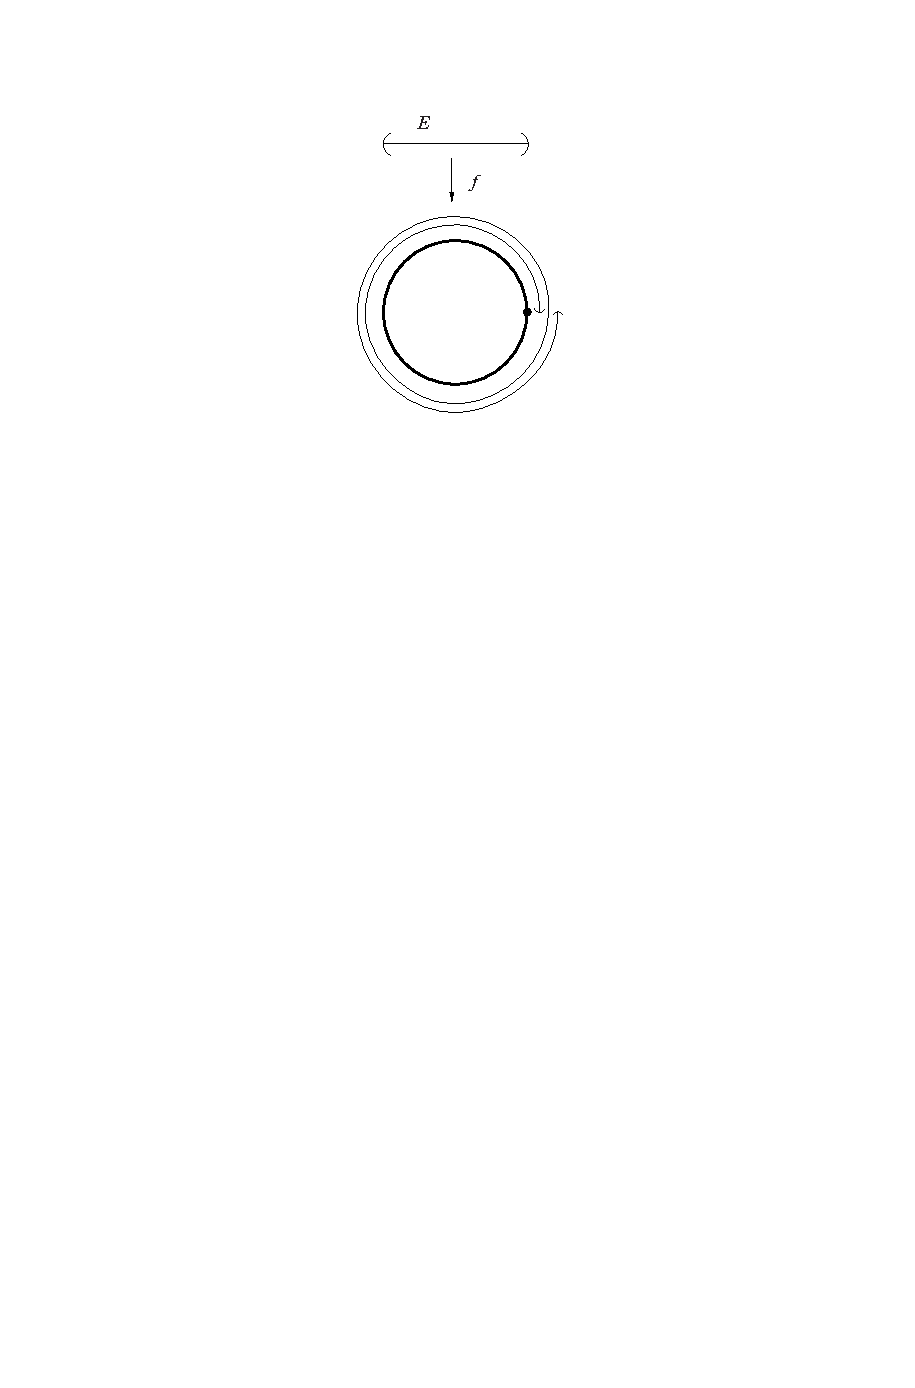
\includegraphics{pictures/covering-counter}
\caption{A surjective local homeomorphism that is not a covering map.}
\end{figure}
\end{example}
In contrast to the example above, a local homeomorphism is indeed a covering map under center conditions. Then following result will be used when we consider covering 
spaces of manifolds.
\begin{proposition}
A proper local homeomorphism between connected, locally path-connected, and compactly generated Hausdorff spaces is a covering map.
\end{proposition}
\begin{proof}
Because $\pi$ is a local diffeomorphism, it is an open map, and because it is proper, it is a closed map (compactly generated Hausfordd space). Thus $\pi(E)$ is both 
open and closed in $M$. Since it is obviously nonempty, it is all of $M$, so $\pi$ is surjective.\par
Let $q\in M$ be arbitrary. Since $\pi$ is a local diffeomorphism, each point of $\pi^{-1}(q)$ has a neighborhood on which $\pi$ is injective, so $\pi^{-1}(q)$ is a 
discrete subset of $E$. Since $\pi$ is proper, $\pi^{-1}(q)$ is also compact, so it is finite. Write $\pi^{-1}(q)=\{p_1,\dots,p_k\}$. For each $i$, there exists a 
neighborhood $V_i$ of $p_i$ on which $\pi$ is a diffeomorphism onto an open subset $U_i\sub M$. Shrinking each $V_i$ if necessary, we may assume also that 
$V_i\cap V_j=\emp$ for $i\neq j$.\par
Now let $U=\bigcap_{i=1}^{k}U_i$, which is a neighborhood of $q$. Then $U\sub U_i$ for all $i$. Because $K:=E-\bigcup_{i=1}^{k}V_i$ is closed in $E$ and $\pi$ is a 
closed map, $\pi(K)$ is closed in $M$. Replacing $U$ by $U-\pi(K)$, we can assume that $U$ also satisfies $\pi^{-1}(U)\sub\bigcup_{i=1}^{k}V_i$. Finally, after replacing 
$U$ by the connected component of $U$ containing $q$, we can assume that $U$ is connected. We will show that $U$ is evenly covered.\par
Let $\widetilde{V}_i=\pi^{-1}(U)\cap V_i$. Then $\pi^{-1}(U)=\widetilde{V}_1\cup\cdots\cup\widetilde{V}_k$. Because $\pi|_{V_i}:V_i\to U_i$ is a diffeomorphism, 
$U\sub U_i$ implies that $\pi|_{\widetilde{V}_i}:\widetilde{V}_i\to U$ is still a diffeomorphism, and in particular $\widetilde{V}_i$ is connected. Because 
$\widetilde{V}_1,\dots,\widetilde{V}_k$ are disjoint connected open subsets of $\pi^{-1}(U)$, they are exactly the components of $\pi^{-1}(U)$.
\end{proof}
For the properness condition, we have the following useful result.
\begin{proposition}
A covering map is proper if and only if it is finite-sheeted.
\end{proposition}
\begin{proof}
Since $\{y\}$ is compect, the fiber $f^{-1}(y)$ is compect, and so it is finite.\par
If $p$ is finite-sheeted, assume $K\sub X$ is compact and let $L:=p^{-1}(K)$, we need to show $L$ is compact. Assume that $\{U_\alpha\}$ is an open cover of $L$. For 
each $x\in K$, choose a fundamental neighborhood $V_x$ such that each component of $p^{-1}(V_x)$ is contained in some $U_\alpha$. This can be done by suitable shrinking 
since $p^{-1}(V_x)$ has finitely many components. Then $K$ has a finite cover $\{V_{x_i}\}_{i=1}^{m}$, and
\[L=p^{-1}(K)\sub p^{-1}(\bigcup_{i=1}^{m}V_{x_i})=\bigcup_{i=1}^{m}p^{-1}(U_{x_i}).\]
Since each $p^{-1}(U_{x_i})$ is contained in a $U_\alpha$, this gives a finite subcover of $\{U_\alpha\}$.
\end{proof}
If $p:X\to Y$ is any surjective continuous map, a \textbf{section} of $p$ is a continuous map $\sigma:Y\to X$ such that $p\circ\sigma=id_Y$ (i.e., a right inverse for $p$). If $U\sub Y$ is an open subset, a \textbf{local section} of $p$ over $U$ is a continuous map $\sigma:U\to X$ such that $p\circ\sigma=id_U$.
\begin{proposition}[\textbf{Existence of Local Sections}]
Let $p:E\to X$ be a covering map. Given any evenly covered open subset $U\sub X$, any $x\in U$, and any $e_0$ in the fiber over $x$, there exists a local section $\sigma:U\to E$ such that $\sigma(x)=e_0$.
\end{proposition}
\begin{proof}
Let $\widetilde{U}_0$ be the sheet of $p^{-1}(U)$ containing $e_0$. Since the restriction of $p$ to $\widetilde{U}_0$ is a homeomorphism, we can just take $\sigma=(p|_{\widetilde{U}_0})^{-1}$.
\end{proof}
\begin{proposition}[\textbf{Cardinality of the fiber}]
For every covering map $p:E\to X$, the cardinality of the fibers $p^{-1}(x)$ is the same for all fibers.
\end{proposition}
\begin{proof}
Define an equivalence relation on $X$ by saying that $x\sim x'$ if and only if $p^{-1}(x)$ and $p^{-1}(x')$ have the same cardinality. Suppose $x\in X$, and let $U$ be an evenly covered neighborhood of $x$. Then each sheet of $p^{-1}(x)$ contains exactly one point of each fiber, so for any $x'\in U$, there are one-to-one correspondences
\[p^{-1}(x)\Longleftrightarrow\text{sheet of }p^{-1}(U)\Longleftrightarrow p^{-1}(x')\]
which shows that $x'\sim x$. It follows that $U$ is contained in the equivalence class
$[x']$, so each equivalence class is open. Thus by the connectness of $X$, there is just one equivalence class.
\end{proof}
If $p:E\to X$ is a covering map, the cardinality of any fiber is called the \textbf{number
of sheets of the covering}.
\subsection{The unique lifting property}
\begin{theorem}[\textbf{Unique Lifting Property}]\label{lift prop}
Let $p:E\to X$ be a covering map. Suppose $Y$ is connected, $\varphi:Y\to X$ is continuous, and $\widetilde{\varphi}_1,\widetilde{\varphi}_2:Y\to E$ are lifts of
$\varphi$ that agree at some point of $Y$. Then $\widetilde{\varphi}_1$ is identically equal to $\widetilde{\varphi}_2$.
\end{theorem}
\begin{proof}
Let $\mathcal{A}=\{x\in X\mid \widetilde{\varphi}_1(x)=\widetilde{\varphi}_2(x)\}$. By hypothesis $\mathcal{A}$ is not empty. Since $X$ is connected, if we can show that $\mathcal{A}$ is open and closed in $X$, it must be all of $X$.\par
To show that $\mathcal{A}$ is open, suppose $x\in\mathcal{A}$. Write $r=\widetilde{\varphi}_1(x)=\widetilde{\varphi}_2(x)$ and $z=p(r)=\varphi(x)$. Let $U\sub X$ be an evenly covered neighborhood of $z$, and let $\widetilde{U}$ be the
component of $p^{-1}(U)$ containing $r$. If we set $V=\widetilde{\varphi}_1^{-1}(\widetilde{U})\cap\widetilde{\varphi}_2^{-1}(\widetilde{U})$, then $V$ is a neighborhood of $x$ on which both $\widetilde{\varphi}_1$ and $\widetilde{\varphi}_3$ take their values in $\widetilde{U}$. Now, the fact that $\widetilde{\varphi}_1$ and $\widetilde{\varphi}_2$ are lifts of $\varphi$ translates to $\varphi=p\circ\widetilde{\varphi}_1=p\circ\widetilde{\varphi}_2$. Since $p$ is
injective on $\widetilde{U}$, we conclude that $\widetilde{\varphi}_1$ and $\widetilde{\varphi}_2$ agree on $V$, which is to say that $V\sub\mathcal{A}$, so $\mathcal{A}$ is open.\par
To show that $\mathcal{A}$ is closed, we show that its complement is open. Suppose $x\notin\mathcal{A}$, and set $r_1=\widetilde{\varphi}_1(x)$ and $r_2=\widetilde{\varphi}_2(x)$, so that $r_1\neq r_2$. As above, let $z=p(r_1)=p(r_2)=\varphi(x)$, and let $U$ be an evenly covered neighborhood of $z$. If $\widetilde{U}_1$ and $\widetilde{U}_2$ are the components of $p^{-1}(U)$ containing $r_1$ and $r_2$, respectively, then $\widetilde{U}_1\cap\widetilde{U}_2=\emp$, and $p$ restricts to a homeomorphism from $\widetilde{U}_1$ to $U$ and from $\widetilde{U}_2$ to $U$. Setting $V=\widetilde{\varphi}_1^{-1}(\widetilde{U})\cap\widetilde{\varphi}_2^{-1}(\widetilde{U})$ we conclude that $\widetilde{\varphi}_1(V)\sub\widetilde{U}_1$ and $\widetilde{\varphi}_2(V)\sub\widetilde{U}_2$, so $\widetilde{\varphi}_1\neq \widetilde{\varphi}_2$ on $V$, which is to say that $V\sub X\setminus\mathcal{A}$. Thus $\mathcal{A}$ is closed, and the proof is complete.
\end{proof}
\begin{theorem}[\textbf{Homotopy Lifting Property}]\label{homotopy lift}
Let $p:E\to X$ be a covering map, and let $Y$ be a locally connected space. Suppose $\varphi_0,\varphi_1:Y\to X$ are continuous maps, $H:Y\times I\to X$ is a homotopy from $\varphi_0$ to $\varphi_1$, and $\widetilde{\varphi}_0:Y\to E$ is any lift of $\varphi_0$. Then there exists a unique lift of $H$ to a homotopy $\widetilde{H}$ satisfying $\widetilde{H}_0=\widetilde{\varphi}_0$. If $H$ is stationary on some subset $A\sub Y$, then so is $\widetilde{H}$.
\end{theorem}
\begin{proof}
We begin by proving a local form of uniqueness for $\widetilde{H}$. Suppose $W$ is any
subset of $Y$, and $\widetilde{H}$, $\widetilde{H}'$ are lifts of $H$ defined on $W\times I$ that agree on $W\times\{0\}$. Then for each $y\in W$, the two maps $t\mapsto\widetilde{H}(y,t)$ and $t\mapsto\widetilde{H}'(y,t)$ are lifts of the path
$t\mapsto H(y,t)$ starting at the same point, so they agree by the unique lifting property. It follows that $\widetilde{H}$ and $\widetilde{H}'$ agree on $W\times I$. In particular, taking $W=Y$, we see that a globally defined lift $\widetilde{H}:Y\times I\to E$ satisfying $\widetilde{H}_0=\widetilde{\varphi}_0$ is unique if it exists.\par
To prove existence, let $y_0\in Y$ be arbitrary. We begin by defining $\widetilde{H}$ on $W\times I$ for some neighborhood $W$ of $y_0$. For each $s\in I$, there exists an evenly covered neighborhood $U$ of the point $H(y_0,s)\in X$. Because $H^{-1}(U)$ is a neighborhood of $(y_0,s)$ and product open subsets form a basis for the product topology on $Y\times I$, there exist open subsets $V\sub Y$ and $J\sub I$ such that $(y_0,s)\in V\times J\sub W\times I$. The collection of all such product sets $V\times J$ is an open cover of $\{y_0\}\times I$, so by compactness finitely many of them, say $V_1,J_1,\cdots,V_m,J_m$, cover $\{y_0\}\times I$. Let $W$ be a connected neighborhood of $y_0$ contained in $V_1\cap\cdots\cap V_m$ (such a neighborhood exists by local connectedness), and let $\delta$ be a Lebesgue number for the open cover $\{J_1,\cdots,J_k\}$ of $I$. If $n$ is a positive integer such that $1/n<\delta$, it follows that for each $j=1,\cdots,n$, the set $W\times[(j-1)/n,j/n]$ is mapped by $H$ into an evenly covered open subset of $X$.\par
We define a lift of $H$ on $W\times I$ inductively as follows. First, choose an evenly
covered open subset $U_1\sub X$ containing $H(W\times[0,1/n])$, and let $\sigma_1:U_1\to E$ be the local section of $p$ satisfying $\sigma_1(\varphi_0(y_0))=\widetilde{\varphi}_0(y_0)$. For $(y,s)\in W\times[0,1/n]$,
define $\widetilde{H}(y,s)=\sigma_1\circ H(y,s)$. This is a composition of continuous maps, and is thus continuous. The map $\widetilde{H}_0:W\to E$ given by $\widetilde{H}_0(y)=H(y,0)$ is a lift of $H_0=\varphi_0$ on a connected domain that agrees with $\widetilde{\varphi}_0$ at the point $y_0$, so by uniqueness of lifts
it agrees with $\varphi_0$ on all of $W$.\par
Now suppose by induction that a continuous lift $\widetilde{H}$ has been defined on $W\times[0,(j-1)/n]$ for some $j\in\{1,\cdots,n\}$. Let $U_j$ be an evenly covered open subset containing $H(W\times[0,(j-1)/n])$ and let $\sigma_j:U_j\to E$ be the local section satisfying $\sigma_j(H(y_0,(j-1)/n))=\widetilde{H}(y_0,(j-1)/n)$. Define $\widetilde{H}(y,s)=\sigma_j\circ H(y,s)$ for $(y,s)\in W\times[(j-1)/n,j/n]$, which is continuous by composition. We need to show that it agrees with our previous definition where the two domains overlap, namely for $(y,s)\in W\times\{(j-1)/n\}$. Note that this set is connected (because $W$ is), and the restrictions to this set of the old and new definitions of $\widetilde{H}$ are both lifts of $H$ that agree at the point $(y_0,(j-1)/n)$. Thus by uniqueness of lifts, they agree everywhere that both are defined. By the pasting lemma, therefore, we obtain a continuous lift of $H$ defined on $W\times[0,j/n]$. This completes the induction and proves that $H$ has a continuous lift on $W\times I$.\par
Every point of $Y$ is contained in some neighborhoodW such that $H$ can be lifted
to $W\times I$. If $W$ and $W'$ are any two such neighborhoods, then the corresponding lifts $\widetilde{H}$ and $\widetilde{H}'$ agree on $(W\cap W')\times I$ by the local uniqueness property proved in the first paragraph. It follows from the pasting lemma that $\widetilde{H}$ is globally well defined and continuous, and by construction it is a lift of $H$ satisfying $\widetilde{H}_0=\widetilde{\varphi}_0$.\par
Finally, if $H$ is stationary on $A\sub Y$, then for each $a\in A$, the path $t\mapsto H(a,t)$ is a constant path at $\varphi_0(a)$ whose unique lift starting at $\widetilde{\varphi}_0(a)$ is the constant path $t\mapsto\widetilde{\varphi}(a)$. It follows that $\widetilde{H}$ is also stationary on $A$.
\end{proof}
\begin{corollary}[\textbf{Path Lifting Property}]\label{path lift}
Let $p:E\to X$ be a covering map. Suppose $f:I\times X$ is any path, and $e\in E$ is any point in the fiber of $p$ over $f(0)$. Then there exists a unique lift $\widetilde{f}:I\to E$ of $f$ such that $\widetilde{f}(0)=e$.
\end{corollary}
\begin{proof}
A path $f$ can be viewed as a homotopy between two maps from a onepoint space $\{\ast\}$ into $S^1$, namely $\ast\mapsto f(0)$ and $\ast\mapsto f(1)$. Thus the existence and uniqueness of $\widetilde{f}$ follow from the homotopy lifting property.
\end{proof}
Whenever $p:E\to X$ is a covering map, we use the following notation for lifts of paths: if $f:I\to X$ is a path and $e\in p^{-1}(f(0))$ then $\widetilde{f}_e:I\to E$ denotes the unique lift of $f$ satisfying $\widetilde{f}_e(0)=e$.
\begin{theorem}[\textbf{Monodromy Theorem}]
Let $p:E\to X$ be a covering map. Suppose $f$ and $g$ are paths in $X$ with the same initial point and the same terminal point, and $\widetilde{f}_e$, $\widetilde{g}_e$ are their lifts with the same initial point $e\in E$.
\begin{itemize}
\item[$(a)$]$\widetilde{f}_e\simeq\widetilde{g}_e$ if and only if $f\simeq g$.
\item[$(a)$]If $f\simeq g$, then $\widetilde{f}_e(1)\simeq\widetilde{g}_e(1)$.
\end{itemize}
\end{theorem}
\begin{proof}
If $\widetilde{f}_e\simeq\widetilde{g}_e$, then $f\simeq g$ because composition with $p$ preserves path homotopy.\par
Conversely, suppose $f\simeq g$, and let $H:I\times I\to X$ be a path homotopy between
them. Then the homotopy lifting property implies that $H$ lifts to a homotopy $H:I\times I\to E$ between $\widetilde{f}$ and some lift of $g$ starting at $e$, which must be equal to $\widetilde{g}$ by the unique lifting property. This proves $(a)$. To prove $(b)$, just note that $f\simeq g$ implies that $\widetilde{f}_e$ and $\widetilde{f}_e$ are path-homotopic by $(a)$, so they have the same terminal point.
\end{proof}
\begin{theorem}[\textbf{Injectivity Theorem}]
Let $p:E\to X$ be a covering map. For any point $e\in E$, the induced homomorphism $p_*:\pi_1(E,e)\to\pi_1(X,p(e))$ is injective.
\end{theorem}
\begin{proof}
Suppose $[f]\in\pi_1(E,e)$ is in the kernel of $p_*$. This means that $p_*[f]=[c_x]$,
where $x=p(e)$. In other words, $p\circ f\simeq c_x$ in $X$. By the monodromy theorem, therefore, any lifts of $p\circ f$ and $c_x$ that start at the same point must be path-homotopic in $E$. Now, $f$ is a lift of $p\circ f$ starting at $e$, and the constant loop $c_e$ is a lift of $c_x$ starting at the same point; therefore, $f\simeq c_e$ in $E$, which means that $[f]=1$.
\end{proof}
The injectivity theorem shows that the fundamental group of a covering space is
isomorphic to a certain subgroup of the fundamental group of the base.We call this the \textbf{subgroup induced by the covering}.
\subsection{The General Lifting Problem}
As our first significant application of the theory of covering spaces, we give a general solution to the lifting problem for covering maps: this is the problem of deciding, given a continuous map $\varphi:Y\to X$, whether $\varphi$ admits a lift $\widetilde{\varphi}$ to a covering space $E$ of $X$. The following theorem reduces this topological problem to an algebraic problem.
\begin{theorem}[\textbf{Lifting Criterion}]\label{lift crit}
Suppose $p:E\to X$ is a covering map. Let $Y$ be a connected and locally path-connected space, and let $\varphi:Y\to X$ be a continuous map. Given any points $y_0\in Y$ and $e_0\in E$ such that $p(e_0)=\varphi(y_0)$, the map $\varphi$ has a lift $\widetilde{\varphi}:Y\to E$ satisfying $\widetilde{\varphi}(y_0)=e_0$ if and only if the subgroup $\varphi_*(\pi_1(Y,y_0))$ of $\pi_1(X,\varphi(y_0))$ is contained in $p_*(\pi_1(E,e_0))$
\end{theorem}
\begin{proof}
The necessity of the algebraic condition is easy to prove (and, in fact, does not require any connectivity assumptions about $Y$). If $\widetilde{\varphi}$ satisfies the conditions in the statement of the theorem, the following diagram commutes:
\[\begin{tikzcd}
&\pi_1(E,e_0)\ar[d,"p_*"]\\
\pi_1(Y,y_0)\ar[ru,"\widetilde{\varphi}_*"]\ar[r,swap,"\varphi_*"]&\pi_1(X,\varphi(y_0))
\end{tikzcd}\]
Therefore, $\varphi_*(\pi_1(Y,y_0))=p_*\circ\widetilde{\varphi}_*(\pi_1(Y,y_0))\sub p_*(\pi_1(E,e_0))$.\par
To prove the converse, we lift $\varphi$ along paths using the path lifting property. If $\widetilde{\varphi}$ does exist, it will have the following property: for any point $y\in Y$ and any path $f$ from $y_0$ to $y$, $\widetilde{\varphi}\circ f$ is a lift of $\varphi\circ f$ starting at $e_0$, and $\widetilde{\varphi}(y)$ is equal to the terminal point of this path. We use this observation to define $\widetilde{\varphi}$: namely, for any $y\in Y$, choose a path $f$ from $y_0$ to $y$, and set
\[\widetilde{\varphi}(y)=\widetilde{(\varphi\circ f)}_{e_0}(1)\]
where, as usual, $\widetilde{(\varphi\circ f)}_{e_0}$ is the lift of $\varphi\circ f$ to a path in $E$ starting at $e_0$. We need to show two things: $(1)$ $\widetilde{\varphi}$ is well defined, independently of the choice of the path $f$; and $(2)$ $\widetilde{\varphi}$ is continuous. Then it is immediate from the definition that 
\[p\circ\widetilde{\varphi}(y)=p\circ\widetilde{(\varphi\circ f)}_{e_0}(1)=\varphi\circ f(1)=\varphi(y),\]
so $\widetilde{\varphi}$ is a lift of $\varphi$.
\begin{itemize}
\item[$(a)$]\textit{$\widetilde{\varphi}$ is well defined}. Suppose $f$ and $f'$ are two paths from $y_0$ to $y$. Then $f'\ast\bar{f}$ is a loop based at $y_0$, so
\[\varphi_*[f'\ast\bar{f}]\in\varphi_*(\pi_1(Y,y_0))\sub p_*(\pi_1(E,e_0)).\]
This means that $\varphi_*[f'\ast\bar{f}]=[p\circ g]$ for some loop $g$ in $E$ based at $e_0$. Thus we have the following path homotopy in $X$:
\[p\circ g\simeq\varphi\circ(f'\ast\bar{f})=(\varphi\circ f')\ast\widebar{(\varphi\circ f)},\]
which implies
\[(p\circ g)\ast(\varphi\circ f)=\varphi\circ f'.\]
By the monodromy theorem, the lifts of these two paths starting at $e_0$ have the same
terminal points. Since the lift of $p\circ g$ is $g$, which starts and ends at $e_0$, this implies
\[\widetilde{(\varphi\circ f')}_{e_0}(1)=g\ast\widetilde{(\varphi\circ f)}_{e_0}(1)=\widetilde{(\varphi\circ f)}_{e_0}(1).\]
so $\widetilde{\varphi}$ is well defined.
\item[$(b)$]\textit{$\widetilde{\varphi}$ is continuous}. Before proving this, we show that $\widetilde{\varphi}$ has one important property of a continuous map: it takes path-connected sets to path-connected sets. Let $V\sub Y$ be path-connected, and $y_1,y_2\in V$ be arbitrary. There is a path $f$ in $Y$ from $y_0$ to $y_1$, and a path $g$ in $V$ from $y_1$ to $y_2$; by definition, $\widetilde{\varphi}$ maps the
path $f\ast g$ to the lift of $(\varphi\circ f)\ast(\varphi\circ g)$. In particular, the lift of $\varphi\circ g$ is a path from $\widetilde{\varphi}(y_1)$ to $\widetilde{\varphi}(y_2)$ that is contained in $\widetilde{\varphi}(V)$. This proves that $\widetilde{\varphi}(V)$ is path-connected.\par
To prove that $\widetilde{\varphi}$ is continuous, it suffices to show that each point in $Y$ has a neighborhood on which $\widetilde{\varphi}$ is continuous. Let $y\in Y$ be arbitrary, let $U$ be an evenly covered neighborhood of $\varphi(y)$, and let $\widetilde{U}$ be the sheet of $p^{-1}(U)$ containing $\widetilde{\varphi}(y)$. If $V$ is the path component of $\varphi^{-1}(U)$ containing $y$, the argument above
shows that $\widetilde{\varphi}$ is a connected subset of $p^{-1}(U)$, and must therefore be contained in $\widetilde{U}$. Since $Y$ is locally path-connected, $V$ is open and thus is a neighborhood of $y$. Let $\sigma:U\to \widetilde{U}$ be the local section of $p$ taking $\varphi(y)$ to $\widetilde{\varphi}(y)$, so $p\circ\varphi$ is the identity on $U$. The following equation holds on $V$:
\[p\circ\widetilde{\varphi}=\varphi=p\circ\sigma\circ\varphi.\]
Both $\widetilde{\varphi}$ and $\sigma\circ\varphi$ map $V$ into $\widetilde{U}$, where $p$ is injective, so this equation implies $\widetilde{\varphi}=\sigma\circ\varphi$ on $V$, which is a composition of continuous maps.
\end{itemize}
\end{proof}
The following corollaries are immediate.
\begin{corollary}[\textbf{Lifting Maps from Simply Connected Spaces}]
If $p:E\to X$ is a covering map and $Y$ is a simply connected and locally path-connected space, then every continuous map $\varphi:Y\to X$ has a lift to $E$. Given any point $y_0\in Y$, the lift can be chosen to take $y_0$ to any point in the fiber over $\varphi(y_0)$.
\end{corollary}
\begin{corollary}
Suppose $p:E\to X$ is a covering map and $E$ is simply connected. For any connected and locally path-connected space $Y$, a continuous map $\varphi:Y\to X$ has a lift to $E$ if and only if $\varphi_*$ is the zero homomorphism for some base point $y_0\in Y$. If this is the case, then the lift can be chosen to take $y_0$ to any point in the fiber over $\varphi(y_0)$.
\end{corollary}
\begin{example}
Consider the $n$-sheeted covering of the circle given by the $n$-th power map $p_n:S^1\to S^1$. It is easy to check that the subgroup of $\pi_1(S^1,1)$ induced by $p_n$ is the cyclic subgroup generated by $[\omega]^n$, where $\omega$ is the loop $\omega(s)=e^{2\pi is}$, whose path homotopy class generates $\pi_1(S^1,1)$. Thus, for any integer $m$, there is a continuous map $f$ making the diagram
\[\begin{tikzcd}
&S^1\ar[d,"p_n"]\\
S^1\ar[ru,dashed,"f"]\ar[r,swap,"p_m"]&S^1
\end{tikzcd}\]
commute if and only if $m=nk$ for some integer $k$. If this is the case, the lift sending $1$ to $1$ is given by $f=p_k$.
\end{example}
\subsection{Group Action}
An action is said to be \textbf{free} if the only element of $G$ that fixes any point in $X$ is the identity. It is easy to check that the action is free if and only if the isotropy group of every point is trivial.\par
Suppose $X$ is a topological space and $G$ is a group acting on $X$. The action is called an \textbf{action by homeomorphisms} if for each $g\in G$, the map $x\mapsto g\cdot x$ is a homeomorphism of $X$. If
in addition $G$ is a topological group, the action is said to be \textbf{continuous} if the map $G\times X\to X$ is continuous. The next proposition explains the relationship between the two concepts.
\begin{proposition}
Suppose $G$ is a topological group acting on a topological space
$X$.
\begin{itemize}
\item[$(a)$]If the action is continuous, then it is an action by homeomorphisms
\item[$(b)$]If $G$ has the discrete topology, then the action is continuous if and only if it is an action by homeomorphisms.
\end{itemize}
\end{proposition}
\begin{proof}
First suppose the action is continuous. This means, in particular, that for each $g\in G$ the map $x\mapsto g\cdot x$ is continuous from $X$ to itself, because it is the composition $x\mapsto(g,x)\mapsto g\cdot x$. Each such map is a homeomorphism, because the definition of
a group action guarantees that it has a continuous inverse $x\mapsto g^{-1}\cdot x$. Thus $G$ acts by homeomorphisms.\par
Now, suppose $G$ has the discrete topology. If $G$ acts by homeomorphisms, then the map $G\times X\to X$ defined by the action is continuous when restricted to each subset of the form $\{g\}\times X$. Since these subsets form an open cover of $G\times X$, this implies that the action is continuous.
\end{proof}
Given an action of a group $G$ on a space $X$ (not necessarily continuous or even by homeomorphisms), we define a relation on $X$ by saying $x_1\sim x_2$ if there is an element $g\in G$ such that $g\cdot x_1=x_2$. This is reflexive because $1\cdot x=x$ for each $x$; it is symmetric because $g\cdot x_1=x_2$ implies $g^{-1}\cdot x_2=x_1$; and it is transitive because $g\cdot x_1=x_2$ and $g'\cdot x_2=x_3$ imply $(g'g)\cdot x_1=x_3$. Thus it is an equivalence relation. The equivalence classes are precisely the orbits of the group action. The resulting quotient space is denoted by $X/G$, and is called the \textbf{orbit space} of the action. If the action is transitive, the orbit space is a single point, so only nontransitive actions yield interesting examples.
\subsection{The Monodromy Action}
\begin{theorem}[\textbf{The Monodromy Action}]
Suppose $p:E\to X$ is a covering map and $x\in X$. There is a transitive right action of $\pi_1(X,x)$ on the fiber $p^{-1}(x)$, called the \textbf{monodromy action}, given by $e\cdot[f]=\widetilde{f}_e(1)$ for $e\in q^{-1}(x)$ and $[f]\in\pi_1(X,x)$.
\end{theorem}
\begin{proof}
If $e$ is any point in $p^{-1}(x)$, the path lifting property shows that every loop
$f$ based at $x$ has a unique lift to a path $\widetilde{f}_e$ starting at $e$. The fact that $f$ is a loop guarantees that $\widetilde{f}_e(1)\in p^{-1}(x)$, and the monodromy theorem guarantees that $\widetilde{f}_e(1)$ depends only on the path class of $f$; therefore, $e\cdot[f]$ is well defined.\par
To see that this is a group action, we need to check two things:
\begin{itemize}
\item[$(\rmnum{1})$] $e\cdot[c_x]=e$.
\item[$(\rmnum{2})$] $(e\cdot[f])\cdot[g]=e\cdot([f]\ast[g])$.
\end{itemize}
For $(\rmnum{1})$, just observe that the constant path $c_e$ is the unique lift of $c_x$ starting at $e$, and therefore $e\cdot[c_x]=c_e(1)=e$. To prove the composition property $(\rmnum{2})$, suppose $f$ and $g$ are two loops based at $x$, and let $z=e\cdot[f]=\widetilde{f}_e(1)$. Then by definition, $(e\cdot[f])\cdot[g]=\widetilde{g}_z(1)$. On the other hand, $\widetilde{f}_e\ast\widetilde{g}_z$ is the lift of $f\ast g$ starting at $e$, which means that
\[e\cdot([f]\ast[g])=e\cdot[f\ast g]=(\widetilde{f}_e\ast\widetilde{g}_z)(1)=\widetilde{g}_z(1)=(e\cdot[f])\cdot[g]\]
Now we need to show that the action is transitive. Because $E$ is path-connected,
any two points $e,e'$ in the fiber over $x$ are joined by a path $h$ in $E$. Setting $f=p\circ h$, we see immediately that $h$ is the lift of $f$ starting at $e$, and therefore $e\cdot[f]=e'$.
\end{proof}
\subsection{Transitive \boldmath{$G$}-Sets}
It turns out that many important properties of the monodromy action are best understood in terms of algebraic properties of sets with transitive group actions. For that reason, we make a short digression to develop a few such properties.\par
If $G$ is a group, a set $S$ endowed with a left or right $G$-action is called a (left or right) \textbf{$\bm{G}$-set}. If the given action is transitive, $S$ is called a \textbf{transitive $\bm{G}$-set}. We restrict our attention in this section to right actions.\par
Suppose $G$ is a group and $S$ is a right $G$-set. For any $s\in S$, the isotropy group of $s$, denoted by $G_s$, is the set of all elements of $G$ that fix $s$:
\[G_s:=\{g\in G\mid s\cdot g=s\}.\]
If $g,g'\in G_s$, then $s\cdot(gg')=s\cdot g'=s$ and $s\cdot g^{-1}=(s\cdot g)\cdot g=s$; thus each isotropy group is a subgroup of $G$.
\begin{proposition}[\textbf{Isotropy Groups of Transitive $\bm{G}$-sets}]\label{G isotropy group}
Suppose $G$ is a group and $S$ is a transitive right $G$-set.
\begin{itemize}
\item[$(a)$]For each $s\in S$ and $g\in G$,
\[G_{s\cdot g}=g^{-1}G_sg.\]
\item[$(b)$]The set $\{G_s:s\in S\}$ of all isotropy groups is exactly one conjugacy class of subgroups of $G$. This conjugacy class is called the \textbf{isotropy type} of $S$.
\end{itemize}
\end{proposition}
\begin{proof}
The proof of $(a)$ is just a computation: for $s\in S$ and $g\in G$,
\begin{align*}
G_{s\cdot g}&=\{g'\in G:(s\cdot g)\cdot g'=s\cdot g\}=\{g'\in G:s\cdot(gg'g^{-1})=s\}\\&=\{g'\in G:gg'g^{-1}\in G_s\}=g^{-1}G_sg.
\end{align*}
Then $(b)$ follows from $(a)$: if $s$ and $s'=s\cdot g$ are any two elements of $S$, their isotropy groups are conjugate by $(a)$; and conversely, if $G_s$ is the isotropy group of some element $s\in S$ and $H=g^{-1}G_sg$ is any subgroup conjugate to $G_s$, then $H$ is the isotropy group of $s\cdot g$.
\end{proof}
Suppose $S_1$ and $S_2$ are right $G$-sets. A map $\varphi:S_1\to S_2$ is said to be \textbf{$\bm{G}$-equivariant} if for each $g\in G$, the operations of applying $\varphi$ and acting on the right by $g$ commute: this means that for all $s\in S_1$ and all $g\in G$,
\[\varphi(s)\cdot g=\varphi(s\cdot g).\]
\begin{proposition}[\textbf{Properties of $\bm{G}$-Equivariant Maps}]\label{G map prop}
Suppose $G$ is a group, and $S_1,S_2$ are transitive right $G$-sets.
\begin{itemize}
\item[$(a)$] Any two $G$-equivariant maps from $S_1$ to $S_2$ that agree on one element of $S_1$ are identical.
\item[$(b)$] If $S_1$ is nonempty, every $G$-equivariant map from $S_1$ to $S_2$ is surjective.
\item[$(c)$] Given $s_1\in S_1$ and $s_2\in S_2$, there exists a $($necessarily unique$)$ $G$-equivariant map $\varphi:S_1\to S_2$ satisfying $\varphi(s_1)=s_2$ if and only if $G_{s_1}\sub G_{s_2}$.
\end{itemize}
\end{proposition}
\begin{proof}
Suppose $\varphi,\varphi':S_1\to S_2$ are $G$-equivariant and $\varphi(s_1)=\varphi'(s_1)$ for some $s_1\in S_1$. Any $s\in S_1$ can be written $s=s_1\cdot g$ for some $g\in G$ (because $G$ acts transitively), and then it follows from equivariance that
\[\varphi(s)=\varphi(s_1\cdot g)=\varphi(s_1)\cdot g=\varphi'(s_1)\cdot g=\varphi'(s_1\cdot g)=\varphi'(s).\]
This proves $(a)$.\par
To prove $(b)$, suppose $S_1\neq \emp$ and $\varphi:S_1\to S_2$ is $G$-equivariant. Choose some $s_1\in S_1$, and let $s_2=\varphi(s_1)$. Given any $s\in S_2$, there exists $g\in G$ such that $s=s_2\cdot g$ by transitivity, and it follows that $\varphi(s_1\cdot g)=\varphi(s_1)\cdot g=s_2\cdot g=s$.\par
To prove $(c)$, suppose first that $\varphi:S_1\to S_2$ is a $G$-equivariant map satisfying $\varphi(s_1)=s_2$. If $g\in G_{s_1}$, then
\[s_2\cdot g=\varphi(s_1)\cdot g=\varphi(s_1\cdot g)=\varphi(s_1)=s_2.\]
which shows that $g\in G_{s_2}$. Conversely, suppose $s_1\in S_1$ and $s_2\in S_2$ are points such that $G_{s_1}\sub G_{s_2}$. Define a map $\varphi:S_1\to S_2$ as follows: given any $s\in S_1$, choose some $g\in G$ such that $s=s_1\cdot g$, and set $\varphi(s)=s_2\cdot g$. To see that this does not depend on the choice of $g$, suppose $g'$ is another element of $G$ such that $s=s_1\cdot g'$. Then $g'g^{-1}$, so $s_2\cdot g'=s_2\cdot g$, which shows that $\varphi$ is well defined. Because $\varphi(s_1\cdot g)=\varphi(s_1)\cdot g$ for all $g\in G$, taking $g=1$ shows that $\varphi(s_1)=s_2$ as desired. To see that $\varphi$ is G-equivariant, let $s\in S_1$ and $h\in G$ be arbitrary, and choose $g$ as above such that $s=s_1\cdot g$. Then $s\cdot h=s_1\cdot(gh)$, so
\[\varphi(s\cdot h)=s_2\cdot(gh)=(s_2\cdot g)\cdot h=\varphi(s)\cdot h.\]
\end{proof}
If $S_1$ and $S_2$ are $G$-sets, a $G$-equivariant bijection $\varphi:S_1\to S_2$ is called a \textbf{$\bm{G}$-isomorphism}. If there exists such a $G$-isomorphism, we say that $S_1$ and $S_2$ are \textbf{$\bm{G}$-isomorphic}.
\begin{proposition}[\textbf{$\bm{G}$-Set Isomorphism Criterion}]\label{G iso crit}
Suppose $S_1$ and $S_2$ are transitive right $G$-sets.
\begin{itemize}
\item[$(a)$] Given $s_1\in S_1$ and $s_2\in S_2$, there exists a $($necessarily unique$)$ $G$-isomorphism $\varphi:S_1\to S_2$ taking $s_1$ to $s_2$ if and only if $G_{s_1}=G_{s_2}$.
\item[$(b)$] $S_1$ and $S_2$ are $G$-isomorphic if and only if they have the same isotropy type.
\end{itemize}
\end{proposition}
\begin{proof}
$(a)$ comes immediately from Proposition~\ref{G map prop}. For $(b)$, assume first that there exists a $G$-isomorphism $\varphi:S_1\to S_2$. Then part $(a)$ shows that $G_{s_1}=G_{s_2}$ for any $s_1\in S_1$ and $s_2=\varphi(s_1)$, so the conjugacy
classes they determine are the same. Conversely, suppose $S_1$ and $S_2$ have the same
isotropy type. This means that $G_{s_1}$ and $G_{s_2}$ are conjugate for any $s_1\in S_1$ and $s_2\in S_2$. Proposition~\ref{G isotropy group}$(b)$ shows that we can 
choose $s'_2\in S_2$ such that $G_{s_1}=G_{s'_2}$, and then part $(a)$ above shows that there is a $G$-isomorphism $\varphi:S_1\to S_2$ taking $s_1$ to $s'_2$.
\end{proof}
If $S$ is a $G$-set, a $G$-isomorphism from $S$ to itself is called a \textbf{$\bm{G}$-automorphism} of $S$. It is easy to check that the set of all $G$-automorphisms of $S$ is a group under composition, called the $G$-automorphism group of $S$ and denoted by $\Aut_G(S)$.\par
Recall that an \textit{orbit} of a group action is the set of all images of a single element under the action by different group elements. The next proposition determines
exactly when two elements of $S$ are in the same orbit of the $G$-automorphism group
\begin{proposition}[\textbf{Orbit Criterion for $\bm{G}$-Automorphisms}]\label{orbit crit G auto}
Suppose $S$ is a transitive right $G$-set. For any $s_1,s_2\in G$, there exists a $($necessarily unique$)$ $\varphi\in\Aut_G(S)$ such that $\varphi(s_1)=s_2$ if and only if the isotropy groups $G_{s_1}$ and $G_{s_2}$ are equal.
\end{proposition}
The last fact about $G$-sets that we need is the following characterization of the
automorphism group of a $G$-set in terms of $G$ itself. It involves the following algebraic notion: if $G$ is a group and $H\sub G$ is a subgroup, the \textbf{normalizer} of $H$ in $G$, denoted by $N_G(H)$, is the set of all elements $\gamma\in G$ such that $\gamma^{-1}H\gamma=H$. The normalizer $N_G(H)$ is easily seen to be a subgroup of $G$ containing $H$; it is in fact the largest subgroup in which $H$ is normal.
\begin{proposition}[\textbf{Algebraic Characterization of $\bm{G}$-Automorphism Groups}]\label{char G auto}
Let $S$ be a transitive right $G$-set, and let $s_0$ be any element of $S$. For each $\gamma\in N_G(G_{s_0})$, there is a unique $G$-automorphism $\varphi\in\Aut_G(S)$ such that $\varphi_\gamma(s_0)=s_0\cdot\gamma$. The map $\gamma\mapsto\varphi_\gamma$ is a surjective group homomorphism from $N_G(G_{s_0})$ to $\Aut_G(S)$ whose kernel is $G_{s_0}$, and thus descends to an isomorphism
\[N_G(G_{s_0})/G_{s_0}\simeq\Aut_G(S).\]
\end{proposition}
\begin{proof}
Suppose $\gamma\in N_G(G_{s_0})$. Then $\gamma^{-1}\in N_G(G_{s_0})$ as well. This implies $G_{s_0}=\gamma^{-1}G_{s_0}\gamma=G_{s_0\cdot\gamma}$. Then Proposition~\ref{G iso crit} shows that there is a unique $G$-automorphism $\varphi$ taking $s_0$ to $s_0\cdot\gamma$.\par 
To show that the map $\gamma\mapsto\varphi_\gamma$ is a homomorphism, let $\gamma_1,\gamma_2\in N_G(G_{s_0})$ be arbitrary. Then
\[\varphi_{\gamma_1}\circ\varphi_{\gamma_2}(s_0)=\varphi_{\gamma_1}(s_0\cdot\gamma_2)=\varphi_{\gamma_1}(s_0)\cdot\gamma_2=(s_0\cdot\gamma_1)\cdot\gamma_2=s_0\cdot(\gamma_1\gamma_2)=\varphi_{\gamma_1\gamma_2}(s_0).\]
Since two $G$-automorphisms that agree on one element are equal, this shows that $\varphi_{\gamma_1}\circ\varphi_{\gamma_2}=\varphi_{\gamma_1\gamma_2}$.\par
To prove surjectivity, let $\varphi\in\Aut_G(S)$ be arbitrary. By transitivity, there is some $\gamma\in G$ such that $s_0=\varphi(s_0)\cdot\gamma$. By Proposition~\ref{G iso crit}, this implies that $G_{s_0}=G_{s_0\cdot\gamma}=\gamma^{-1}G_{s_0}\gamma$, so $\gamma\in N_G(G_{s_0})$. It follows that there is a unique $G$-automorphism $\varphi_\Gamma$ such that $\varphi_\gamma(s_0)=s_0\cdot\gamma$ and since $\varphi$ is such an automorphism, we must have $\varphi=\varphi_\gamma$.\par
Finally,
\[\varphi_\gamma=id_S\iff\varphi_\gamma(s_0)=s_0\iff s_0\cdot\gamma=s_0\iff\gamma\in G_{s_0}.\]
which shows that the kernel of the map $\gamma\mapsto\varphi_\gamma$ is exactly $G_{s_0}$.
\end{proof}
\subsection{Properties of the Monodromy Action}
Now we are ready to apply the preceding results about $G$-sets to the special case of
the monodromy action. First we need to identify the isotropy groups of that action.
\begin{theorem}[\textbf{Isotropy Groups of the Monodromy Action}]\label{iso group of monodromy}
Suppose $p:E\to X$ is a covering map and $x\in X$. For each $e\in p^{-1}(x)$, the isotropy group of $e$ under the monodromy action is $p_*(\pi_1(E,e))\sub\pi_1(X,x)$.
\end{theorem}
\begin{proof}
Let $e\in p^{-1}(x)$ be arbitrary, and suppose first that $[f]$ is in the isotropy
group of $e$. This means $\widetilde{f}_e(1)=e$, which is to say that $\widetilde{f}_e$ is a loop and thus represents an element of $\pi_1(E,e)$. It is easy to check that $p_*[\widetilde{f}_e]=[f]$, so $[f]\in p_*(\pi_1(E,e))$. Conversely, if $[f]\in p_*(\pi_1(E,e))$, then there is a loop $g:I\to E$ based at $e$ such that $p_*[g]=[f]$, which means that $p\circ g=f$. If we let $f'=p\circ g$, then $g=\widetilde{f}'_e$ (by uniqueness of lifts), and $e\cdot[f]=e\cdot[f']=\widetilde{f'}_e(1)=g(1)=e$, which means that $[f]$ is in the isotropy group of $e$.
\end{proof}
\begin{corollary}\label{monodromy action free iff}
Suppose $p:E\to X$ is a covering map. The monodromy action is free on each fiber of $p$ if and only if $E$ is simply connected.
\end{corollary}
\begin{proof}
The action is free if and only if each isotropy group is trivial, which by Theorem~\ref{iso group of monodromy} is equivalent to $p_*(\pi_1(E,e))$ being the trivial group for each $e$ in the fiber. Since $p_*$ is injective, this is true if and only if $E$ is simply connected.
\end{proof}
\begin{corollary}\label{card fund fiber}
Suppose $p:E\to X$ is a covering map and $E$ is simply connected. Then each fiber of $p$ has the same cardinality as the fundamental group of $X$.
\end{corollary}
\begin{proof}
By the previous corollary, the monodromy action is free. Choose a base point $x\in X$ and a point $e$ in the fiber over $x$, and consider the map $\pi_1(X,x)\mapsto p^{-1}(x)$ given by $[f]\mapsto e\cdot[f]$. It is surjective because the monodromy action is transitive, and it is injective because the action is free.
\end{proof}
\begin{example}
Suppose $n>1$. Since the quatient map $p:S^n\to\P^n$ is a two-sheeted covering and $S^n$ is simply connected, Corollary~\ref{card fund fiber} shows that $\pi_1(\P^n)$ is a two-element group, which must therefore be isomorphic to $\Z/2\Z$.
\end{example}
\begin{corollary}[\textbf{Coverings of Simply Connected Spaces}]
If $X$ is a simply connected space, every covering map $p:E\to X$ is a homeomorphism.
\end{corollary}
\begin{proof}
The injectivity theorem shows that $E$ is also simply connected. Then Corollary~\ref{card fund fiber} shows that the cardinality of the fibers is $1$, so $p$ is injective. Thus it is a homeomorphism.
\end{proof}
It is important to remember that in general, the subgroup induced by a covering depends not only on the covering but also on the choice of base point. As the next theorem shows, the subgroup may change when we change base point within a given fiber, but it can change only in a very limited way.
\begin{theorem}[\textbf{Conjugacy Theorem}]
Let $p:E\to X$ be a covering map. For any $x\in X$, as $e$ varies over the fiber $p^{-1}(x)$, the set of induced subgroups $p_*(\pi_1(E,e))$ is exactly one conjugacy class in $\pi_1(X,x)$.
\end{theorem}
\begin{proof}
Given $x\in X$, Theorem~\ref{iso group of monodromy} shows that the set of subgroups $p_*(\pi_1(E,e))$ as $e$ varies over $p^{-1}(x)$ is equal to the set of isotropy groups of points in $p^{-1}(x)$ under the monodromy action. Then Proposition~\ref{G isotropy group}$(b)$ shows that this set of isotropy groups is exactly one conjugacy class.
\end{proof}
There is an important special case in which the subgroup $p_*(\pi_1(E,e))$ does not depend on the choice of base point within a given fiber. A covering map $p:E\to X$ is
called a \textbf{normal covering} if the induced subgroup $p_*(\pi_1(E,e))$ is a normal subgroup of $\pi_1(X,p(e))$ for some $e\in E$. (Normal coverings are called \textbf{regular coverings} by some authors.)
\begin{proposition}[\textbf{Characterizations of Normal Coverings}]\label{char nomral cover}
Suppose $p:E\to X$ is a covering map. Then the following are equivalent:
\begin{itemize}
\item[$(a)$] The subgroup $p_*(\pi_1(E,e))$ is normal for some $e\in E$ $($i.e., $p$ is normal$)$.
\item[$(b)$] For some $x\in X$, the subgroups $p_*(\pi_1(E,e))$ are the same for all $e\in p^{-1}(x)$.
\item[$(c)$] For every $x\in X$, the subgroups $p_*(\pi_1(E,e))$ are the same for all $e\in p^{-1}(x)$.
\item[$(d)$] The subgroup $p_*(\pi_1(E,e))$ is normal for every $e\in E$.
\end{itemize}
\end{proposition}
\begin{proof}
Because a subgroup is normal if and only if it is the sole member of its conjugacy class, the implications $(d)\Rightarrow(c)\Rightarrow(b)\Rightarrow(a)$ are easy consequences of the conjugacy theorem. Thus we need only prove $(a)\Rightarrow(d)$.\par
Assume that $(a)$ holds, and let $e_0\in E$ be a point such that $p_*(\pi_1(E,e_0))$ is normal in $\pi_1(X,x_0)$, where $x_0=p(e_0)$. Suppose $e$ is any other point of $E$, and let $x=p(e)$. Let $h$ be a path in $E$ from $e_0$ to $e$, and set $g=p\circ h$, which is a path in $X$ from $x_0$ to $x$.We have four maps
\[\begin{tikzcd}
\pi_1(E,e_0)\ar[d,"p_*"]\ar[r,"\varPhi_h"]&\pi_1(E,e)\ar[d,"p_*"]\\
\pi_1(X,x_0)\ar[r,"\varPhi_g"]&\pi_1(X,x)\\
\end{tikzcd}\]
The top and bottom rows are isomorphisms, and the diagram commutes because
\[p_*\circ\varPhi_h[f]=p_*[\bar{h}\ast f\ast h]=[\bar{g}]\ast p_*[f]\ast[g]=\varPhi_g\circ p_*[f].\]
It follows that $\varPhi_g$ takes $p_*(\pi_1(E,e_0))$ to $p_*(\pi_1(E,e))$. Since an isomorphism takes normal subgroups to normal subgroups, $(d)$ follows.
\end{proof}
\subsection{Covering Homomorphisms}
Suppose $p_1:E_1\to X$, $p_2:E_2\to X$ are two coverings of the same topological
space $X$. A covering homomorphism from $p_1$ to $p_2$ is a continuous map $\varphi:E_1\to E_2$ such that $p_2\circ\varphi=p_1$:
\[\begin{tikzcd}
E_1\ar[rd,swap,"p_1"]\ar[rr,"\varphi"]&&E_2\ar[ld,"p_2"]\\
&X&
\end{tikzcd}\]
A covering homomorphism that is also a homeomorphism is said to be a \textbf{covering
isomorphism}. It is easy to see that in this case the inverse map is also a covering isomorphism.\par
We say two coverings are isomorphic if there is a covering isomorphism between them; this is an equivalence relation on the class of coverings of $X$.
\begin{proposition}[\textbf{Properties of Covering Homomorphisms}]\label{covering homo}
Let $p_1:E_1\to X$ and $p_2:E_2\to X$ be coverings of the same space $X$.
\begin{itemize}
\item[$(a)$] If two covering homomorphisms from $p_1$ to $p_2$ agree at one point of $E_1$, then they are equal.
\item[$(b)$] Given $x\in X$, any covering homomorphism from $p_1$ to $p_2$ restricts to a $\pi_1(X,x)$-equivariant map from $p_1^{-1}(x)$ to $p^{-1}_2(x)$ $($with respect to the monodromy actions$)$.
\item[$(c)$] Every covering homomorphism is itself a covering map.
\end{itemize}
\end{proposition}
\begin{proof}
A covering homomorphism from $p_1$ to $p_2$ can also be viewed as a lift of $p_1$:
\[\begin{tikzcd}
&E_2\ar[d,"p_2"]\\
E_1\ar[ru,"\varphi"]\ar[r,swap,"p_1"]&X
\end{tikzcd}\]
Thus $(a)$ follows from the unique lifting property.\par
To prove $(b)$, suppose $\varphi:E_1\to E_2$ is a covering homomorphism from $p_1$ to $p_2$. Note first that the definition implies that $\varphi$ maps $p^{-1}_1(x)$ to $p^{-1}_2(x)$. Given $x\in X$, $e\in p_1^{-1}(x)$, and $[f]\in\pi_1(X,x)$, we need to show that $\varphi(e\cdot[f])=\varphi(e)\cdot[f]$. Let $\widetilde{f}_e$ be the lift of $f$ to a path in $E_1$ starting at $e$, and consider the path $\varphi\circ\widetilde{f}_e$ in $E_2$. Its initial point is $\varphi\circ\widetilde{f}_e(0)=\varphi(e)$, and it satisfies $p_2\circ\varphi\circ\widetilde{f}_e=p_1\circ\widetilde{f}_e=f$, so $\varphi\circ\widetilde{f}_e$ is the lift of $f$ to $E_2$ starting at $\varphi(e)$. Therefore
\[\varphi(e)\cdot[f]=(\varphi\circ\widetilde{f}_e)(1)=\varphi(\widetilde{f}_e(1))=\varphi(e\cdot[f]).\]
Finally, we prove $(c)$. Let $\varphi:E_1\to E_2$ be a covering homomorphism. First we
have to show that $\varphi$ is surjective. Given $e\in E_2$, let $x=p_2(e)\in X$. The fact that $p_1$ is surjective means that $p_1^{-1}(x)$ is nonempty, and part $(b)$ implies that $\varphi$ restricts to a $\pi_1(X,x)$-equivariant map from $p_1^{-1}(x)$ to $p_1^{-1}(x)$. By Proposition~\ref{G map prop}$(b)$, this restricted map is surjective, which means in particular that $e$ is in the image of $\varphi$.\par 
To show that $\varphi$ is a covering map, let $e\in E_2$ be arbitrary; let $x=p_2(e)\in X$; let $U_1,U_2\sub X$ be neighborhoods of $x$ that are evenly covered by $p_1$ and $p_2$, respectively; and let $V$ be the component of $U_1\cap U_2$ containing $x$. Thus $V$ is a neighborhood of $x$ that is evenly covered by both $p_1$ and $p_2$.\par
Let $U$ be the component of $p_2^{-1}(V)$ containing $e$. We need to show that the
components of $\varphi^{-1}(U)$ are mapped homeomorphically onto $U$ by $\varphi$. Consider the restrictions of $p_1$ and $\varphi$ to $p_1^{-1}(V)$. Since $U$ is
both open and closed in $p_2^{-1}(V)$, it follows that $U$ is both open and closed in $q_1^{-1}(V)$, and is thus a union of components. On any such component $U_\alpha$, the following diagram commutes:
\[\begin{tikzcd}
U_\alpha\ar[dd,"p_1"]\ar[rd,"\varphi"]&\\
&U\ar[ld,"p_2"]\\
V
\end{tikzcd}\]
Since $p_1$ and $p_2$ are homeomorphisms in this diagram, so is $\varphi$.
\end{proof}
The key to determining when two covering spaces are isomorphic is to decide when there are covering homomorphisms between them. This question is answered by the following theorem.
\begin{theorem}[\textbf{Covering Homomorphism Criterion}]
Let $p_1:E_1\to X$ and $p_2:E_2\to X$ be two coverings of the same space $X$, and suppose $e_1\in E_1$ and $e_2\in E_2$ are base points such that $p_1(e_1)=p_2(e_2)$. There exists a covering homomorphism from $p_1$ to $p_2$ taking $e_1$ to $e_2$ if and only if $p_{1*}(\pi_1(E_1,e_1))\sub p_{2*}(\pi_1(E_2,e_2))$.
\end{theorem}
\begin{proof}
Because a covering homomorphism from $p_1$ to $p_2$ is a lift of $p_1$, both the necessity and the sufficiency of the subgroup condition follow from the lifting criterion. (Theorem~\ref{lift crit})
\end{proof}
\begin{example}
Consider the following two coverings of $T^2$: the first is $\eps^2:\R^2\to T^2$; and
the second is the map $q:S^1\times\R\to T^2$ given by $p(z,e)=(z,\eps(e))$ $(\eps(s)=e^{2\pi is})$. Identifying $\pi_1(T^2)$ with $\Z\times\Z$, we see that $(\eps)^2_*(\pi_1(\R^2))$ is trivial, while $q_*(\pi_1(S^1\times\R))=\Z\times\{0\}$. Therefore, there exists a covering homomorphism from $\eps^2$ to $q$. $($Why do the base points not matter?$)$ It is easy to check that $\varphi(x,e)=(\eps(x),e)$ is such a homomorphism.
\end{example}
The following theorem completely solves the uniqueness question for covering
spaces up to isomorphism.
\begin{theorem}[\textbf{Covering Isomorphism Criterion}]\label{cover iso crit}
Suppose $p_1:E_1\to X$ and $p_2:E_2\to X$ are two coverings of the same space $X$.
\begin{itemize}
\item[$(a)$] Given $e_1\in E_1$ and $e_2\in E_2$ such that $p_1(e_1)=p_2(e_2)$, there exists a $($necessarily unique$)$ covering isomorphism from $p_1$ to $p_2$ taking $e_1$ to $e_2$ if and only if $p_{1*}(\pi_1(E_1,e_1))=p_{2*}(\pi_1(E_2,e_2))$.
\item[$(b)$] The coverings $p_1$ and $p_2$ are isomorphic if and only if for some $x\in X$, the conjugacy classes of subgroups of $\pi_1(X,x)$ induced by $p_1$ and $p_2$ are the same. If this is the case, these conjugacy classes are the same for every $x\in X$.
\end{itemize}
\end{theorem}
\begin{proof}
First we prove $(a)$. Suppose there exists a covering isomorphism $\varphi:E_1\to E_2$ such that $\varphi(e_1)=e_2$, and let $x=p_1(e_1)=p_2(e_2)$. By Proposition~\ref{covering homo}$(b)$, $\varphi$ restricts to a $\pi_1(X,x)$-isomorphism from $p_1^{-1}(x)$ to $p_2^{-1}(x)$ taking $e_1$ to $e_2$, so it follows from Proposition~\ref{G iso crit} that the isotropy groups of $e_1$ and $e_2$, namely $p_{1*}(\pi_1(E_1,e_1))$ and $p_{2*}(\pi_1(E_2,e_2))$, are equal.\par
Conversely, suppose $p_{1*}(\pi_1(E_1,e_1))=p_{2*}(\pi_1(E_2,e_2))$. Then by the covering homomorphism criterion, there exist covering homomorphisms $\varphi:E_1\to E_2$ and $\psi:E_2\to E_1$, with $\varphi(e_1)=e_2$ and $\psi(e_2)=e_1$. The composite map $\psi\circ\varphi$ is a covering homomorphism from $E_1$ to itself that fixes $e_1$, so it is the identity. Similarly, $\varphi\circ\psi$ is the identity, so $\varphi$ is the required covering isomorphism.\par
To prove $(b)$, suppose first that the two coverings are isomorphic. For any $x\in X$, the covering isomorphism restricts to a $\pi_1(X,x)$-isomorphism from $p_1^{-1}(x)$ to $p_2^{-1}(x)$, so these fibers have the same isotropy type as $\pi_1(X,x)$-sets by Proposition~\ref{G iso crit}. Because the isotropy groups of the monodromy action are exactly the induced subgroups of the covering, it follows that $p_1$ and $p_2$ induce the same conjugacy class of subgroups of $\pi_1(X,x)$.\par
Conversely, suppose that $p_1$ and $p_2$ induce the same conjugacy class of subgroups
for some $x\in X$. Choose $e_1\in p_1^{-1}(x)$ arbitrarily. By the conjugacy theorem, there is some $e_2\in p_1^{-1}(x)$ such that $p_{2*}(\pi_1(E_2,e_2))=p_{1*}(\pi_1(E_1,e_1))$, and then part $(a)$ shows that there is a covering isomorphism from $p_1$ to $p_2$ taking $e_1$ to $e_2$. The argument in the preceding paragraph then shows that the two coverings induce the same conjugacy class in $\pi_1(X,x')$ for any other base point $x'\in X$ as well.
\end{proof}
\vspace{5mm}
\subsection{The Universal Covering Space}
When the results of the preceding section are applied to simply connected covering
spaces, they yield some extremely useful results.
\begin{proposition}[\textbf{Universal property of Simply Connected Coverings}]\label{universal cover prop}
\mbox{}
\begin{itemize}
\item[$(a)$] Let $p:E\to X$ be a covering map with $E$ simply connected. If $p':E'\to X$ is any covering, there exists a covering map $Q:E\to E'$ such that the following
diagram commutes:
\[\begin{tikzcd}
E\ar[dd,"p"]\ar[rd,dashed,"Q"]&\\
&E'\ar[ld,"p'"]\\
X
\end{tikzcd}\]
\item[$(b)$] Any two simply connected coverings of the same space are isomorphic.
\end{itemize}
\end{proposition}
\begin{proof}
Since the trivial subgroup is contained in every other subgroup, part $(a)$ follows
from the covering homomorphism criterion and the fact that every covering
homomorphism is a covering map. Part $(b)$ follows immediately from the covering
isomorphism criterion.
\end{proof}
Part $(a)$ of this proposition says that a simply connected covering space covers
every other covering space of $X$. Because of this, any covering of $X$ by a simply
connected space $\widetilde{X}$ (which by $(b)$ is unique up to isomorphism) is called a \textbf{universal covering}, and $\widetilde{X}$is called the \textbf{universal covering space} of $X$.
\begin{example}
The universal covering space of $S^1$ is $\R$, with the exponential quotient map $\eps$ as the covering map. Similarly, for $n\geq 2$ we constructed a covering map $\eps^n:\R^n\to T^n$, so the universal covering space of the $n$-torus is $\R^n$. The universal covering space of $\P^n$ for $n\geq2$ is $S^n$ by the quotient map.
\end{example}
We say that a space $X$ is \textbf{locally simply connected} if it admits a basis of simply connected open subsets. Clearly, a locally simply connected space is locally path-connected, because simply connected sets are pathconnected. Every manifold is locally simply connected, because it has a basis of coordinate balls.\par
We say that a space $X$ is \textbf{semi-locally simply connected} if every point $x\in X$ has a neighborhood $U$ such that $\pi_1(U,x)\to\pi_1(X,x)$ is the trivial homomorphism. Such a neighborhood $U$ is called \textbf{relatively simply connected}. If $U$ is relatively simply connected, then so is every subset of $U$, so a semilocally simply connected space actually has a basis of relatively simply connected open subsets. Clearly every locally simply connected space is semilocally simply connected.
\begin{theorem}\label{existence universal cover}
If $X$ is connected, locally path connected, and semi-locally simply connected, then $X$ has a universal cover.
\end{theorem}
\begin{proof}
To get an idea how to proceed, suppose for a moment that $X$ does have a
universal covering $p:\widetilde{X}\to X$. The key fact is that once we choose base points $\widetilde{x}_0\in\widetilde{X}$ and $x_0=p(x)\in X$, the fiber $p^{-1}(x)$ over any $x\in X$ is in one-to-one correspondence with path classes from $x_0$ to $x$. To see why, define a map $E$ from the set of such path classes to $p^{-1}(x)$ by sending $[f]$ to the terminal point of the lift of $f$ starting at $\widetilde{x}_0$. Since lifts of homotopic paths have the same terminal point by the monodromy theorem, $E$ is well defined. $E$ is surjective, because given any $\widetilde{x}$ in the fiber over $x$, there is a path $\widetilde{f}$ from $\widetilde{x}_0$ to $\widetilde{x}$, and then $p\circ\widetilde{f}$ is a path from $x_0$ to $x$ whose lift ends at $\widetilde{x}$. Injectivity of $E$ follows from the fact that $\widetilde{X}$ is simply connected: if $f_1$, $f_2$ are two paths from $x_0$ to $x$ whose lifts $\widetilde{f}_1,\widetilde{f}_2$ end at the same point, then $\widetilde{f}_1$ and $\widetilde{f}_2$ are path-homotopic, and therefore so are $f_1=p\circ\widetilde{f}_2$ and $f_2=p\circ\widetilde{f}_2$. (Recall $\R$ as a universal covering of $S^1$, in fact we use this observation to compute the fundamental group of $S^1$.)\par
Fix a base point $x_0\in X$. We turn the properties of paths that must hold in a universal cover into a construction. Define $\widetilde{X}$ to be the set of homotopy classes of paths $[f]$ in $X$ that start at $x_0$ and define $p:\widetilde{X}\to X$ by $p([f])=f(1)$. We prove that $\widetilde{X}$ has the required properties in a series of steps.\par
\begin{itemize}
\item[$(1)$] \textit{Topologize $\widetilde{X}$}. The topology of $X$ has a basis $\mathcal{U}$ consisting of path connected open subsets $U$ such that $\pi_1(U,u)\to\pi_1(X,u)$ is trivial for all $u\in U$. Since every loop in $U$ is homotopic in $X$ to the trivial loop, any two paths from $u$ to $u'$ in such a $U$ are homotopic in $X$. We shall topologize $\widetilde{X}$ so that $p$ is a cover with these $U$ as fundamental neighborhoods. For a path $f$ in $X$ that starts at $x_0$ and ends in $U$ for some $U\in\mathcal{U}$, define a subset $U_{[f]}$ of $\widetilde{X}$ by
\[U_{[f]}=\{[g]\mid [g]=[f\ast c]\text{ for some path }c:I\to U\}.\]
Let $\mathcal{B}$ denote the collection of all such $U_{[f]}$, then we prove that $\mathcal{B}$ is a basis for a topology on $\widetilde{X}$.\par
First, since $X$ is semi-locally simply connected, for each $[f]\in\widetilde{X}$, there exists a $U\in\mathcal{U}$ containing $f(1)$, and clearly $[f]\in U_{[f]}$. Thus the union of all the sets in $\mathcal{B}$ is $\widetilde{X}$.\par
Then, suppose $U_{[f]}$ and $U'_{[f']}$ are two sets in $\mathcal{B}$ and $[g]$ is in their intersection, then $g\simeq f\ast a\simeq f'\ast b$, where $a,b$ are paths in $U$, $U'$ respectively. Let $W\in\mathcal{U}$ be a path connected neighborhood of $g(1)$ contained in $U\cap V$ (such a neighborhood exists because $X$ is semi-locally simply connected).If $[g\ast c]\in W_{[g]}$, then $[g\ast c]=[f\ast a\ast c]=[f'\ast b\ast c]$, so $[g\ast c]\in U_{[f]}$ and $[g\ast c]\in U_{[f']}$. Thus $W_{[g]}$ is a basis set contained in $U_{[f]}\cap U'_{[f']}$. From now on, we endow $\widetilde{X}$ with the topology generated by $\mathcal{B}$.
\item[$(2)$] \textit{$\widetilde{X}$ is path-connected}. Let $[f]\in\widetilde{X}$ be arbitrary.We will show that there is a path in $\widetilde{X}$ from $\widetilde{x}_0$ to $[f]$, where $\widetilde{x}_0=[c_{x_0}]$.\par
For each $0\leq t\leq 1$, define $f_t:I\to X$ by
\[f_t(s)=f(ts).\]
so $f_t$ is a path in $X$ from $x_0$ to $f(t)$. Then define $\widetilde{f}:I\to\widetilde{X}$ by
\[\widetilde{f}(t)=[f_t].\]
Clearly, $\widetilde{f}(0)=[f_0]=\widetilde{x}_0$, and $\widetilde{f}(1)=[f_1]=[f]$. So we need only show that $\widetilde{f}$ is continuous; for this it suffices to show that the preimage under $\widetilde{f}$ of every basis $U_{[h]}\sub\widetilde{X}$ is open. Let $t_0\in I$ be a point such that $\widetilde{f}(t_0)\in U_{[h]}$. This means that $f_{t_0}\simeq h\ast c$ for some path $c$ lying in $U$, and in particular that $f(t_0)=f_{t_0}(1)\in U$. For each $0\leq t\leq1$, define a path $f_{t_0t}$ by
\[f_{t_0t}(s)=f(t_0+s(t-t_0)).\]
This path just follows $f$ from $f_{t_0}$ to $f(t)$, so $f_{t_0}\ast f_{t_0t}$ is easily seen to be pathhomotopic to $f_t$.\par
By continuity of $f$, there is some $\delta>0$ such that $f(t_0-\delta,t_0+\delta)\sub U$. If $t\in(t_0-\delta,t_0+\delta)$, then
\[f_t\simeq f_{t_0}\ast f_{t_0t}\simeq h\ast c\ast f_{t_0t}.\]
from which it follows that
\[\widetilde{f}(t)=[f_t]=[h\ast c\ast f_{t_0t}]\in U_{[h]}.\]
This shows that $\widetilde{f}^{-1}(U_{[h]})$ contains the set $(t_0-\delta,t_0+\delta)$, thus $\widetilde{f}^{-1}(U_{[h]})$ is open, which means $\widetilde{f}$ is continuous.
\item[$(3)$] \textit{$p$ is a covering map}. Let $U\sub X$ be any path connected open subset in $\mathcal{U}$. As we have mensioned, we will show that $U$ is evenly covered.\par
Choose any point $x_1\in U$. We begin by showing that $p^{-1}(U)$ is the disjoint union of the sets $U_{[f]}$ as $[f]$ varies over all the distinct path classes from $x_0$ to $x_1$. It follows immediately from the definition of $p$ that $p(U_{[f]})\sub U$, so $\bigcup_{[f]}U_{[f]}\sub p^{-1}(U)$. Conversely, if $[g]\in p^{-1}(U)$, then $g(1)=p([g])\in U$, so there is a path $b$ in $U$ from $g(1)$ to $x_1$, and $[g]=[g\ast b\ast\bar{b}]\in U_{[g\ast b]}$. This proves that $p^{-1}(U)=\bigcup_{[f]}U_{[f]}$.\par
This shows, in particular, that $p$ is continuous: $X$ has a basis $\mathcal{U}$, and the preimage under $p$ of each such set is a union of basis sets and therefore open. And $p$ is clearly surjective, because each $x\in X$ is equal to $p([g])$ for any path $g$ from $x_0$ to $x$.\par
Next we show that $p$ is a homeomorphism from each set $U_{[f]}$ to $U$. It is surjective because for each $x\in U$ there is a path $a$ from $f(1)$ to $x$ in $U$, so $x=p([f\ast a])\in q(U_{[f]})$. To see that it is injective, let $[g],[g']\in U_{[f]}$, and suppose $p([g])=p([g'])$, or in other words, $g(1)=g'(1)$. Then by the definition of $U_{[f]}$, $g\simeq f\ast a$ and $g\simeq f\ast a'$ for some paths $a,a'$ in $U$ from $f(1)$ to $g(1)$. Since $U$ is relatively simply connected, $a\simeq a'$ and therefore $[g]=[g']$. Finally, $p$ is an open map because it takes basis open subsets to open subsets, and therefore $p:U_{[f]}\to U$ is a homeomorphism.\par
Each set $U_{[f]}$ is open by definition, and each is path-connected because it
is homeomorphic to the path-connected set $U$. It follows that $\widetilde{X}$ is locally pathconnected. To complete the proof that $p$ is a covering map, we need to show that for any two paths $f$ and $f'$ with $f(1)\in U$, $f'(1)\in U$, the sets $U_{[f]}$ and $U_{[f']}$ are either equal or disjoint. If they are not disjoint, there exists $[g]\in U_{[f]}\cap U_{[f']}$, so $[g]=[f\ast a]$ for a path $a$ in $U$. Then the element in $U_{[g]}$ have the form $[f\ast a\ast h]$ and hence lie in $U_{[f]}$, while elements of $U_{[f]}$ have the form $[f\ast h] = [f\ast a\ast \bar{a}\ast h]=[g\ast\bar{a}\ast h]$ and hence lie in $U_{[g]}$. This shows $U_{[f]}=U_{[g]}$, and similarly $U_{[f']}=U_{[g]}=U_{[f]}$.
\item[$(4)$] \textit{$\widetilde{X}$ is simply connected}. Suppose $F:I\to\widetilde{X}$ is a loop based at $\widetilde{x}_0$. Let $f=p\circ F$, so $F$ is a lift of $f$. If we write $\widetilde{f}=[f_t]$ as in $(2)$, then $p\circ\widetilde{f}=p([f_t])=f_t(1)=f(t)$, so $\widetilde{f}$ is also a lift of $f$ starting at $\widetilde{f}$. By the unique lifting property, $F=\widetilde{f}$. Since $F$ is a loop, 
\[[c_{x_0}]=\widetilde{x}_0=F(1)=\widetilde{f}(1)=[f_1]=[f],\]
so $f$ is null-homotopic. By the monodromy theorem, this means that $F$ is nullhomotopic as well.
\end{itemize}
\end{proof}
\begin{remark}
In fact, assume $p:\widetilde{X}\to X$ is a covering space of $X$ with $\widetilde{X}$ simply-connected. Every point $x\in X$ has a neighborhood $U$ having a lift $\widetilde{U}\sub\widetilde{X}$ projecting homeomorphically to $U$ by $p$. Each loop in $U$ lifts to a loop in $\widetilde{U}$, and the lifted loop is nullhomotopic in $\widetilde{U}$ since $\pi_1(\widetilde{X})=0$. So, composing this
nullhomotopy with $p$, the original loop in $U$ is nullhomotopic in $X$. So the condition in Theorem~\ref{existence universal cover} is necessary.
\end{remark}
\subsection{Exercise}
\begin{exercise}
Let $S$ be the following subset of $\C^2$:
\[S=\{(z,w):w^2=z,w\neq0\}\]
Show that the projection $\pi_1:\C^2\to\C$ onto the first coordinate restricts to a two-sheeted covering map $p:S\to\C\setminus\{0\}$.
\end{exercise}
\begin{proof}
The map $\sqrt{z}$ is locally defined.
\end{proof}
\begin{exercise}
Show that there is a two-sheeted covering of the Klein bottle by the torus.
\end{exercise}
\begin{lemma}
Let $X$ be a connected, locally path connected space, let $f:X\to X$ be a homeomorphism such that $f^n=id_X$ and $f^m(x)\neq x$ for $0<m<n$. Define an equivalence relation on $X$ by
\[x\sim x'\iff \exists\ell\in\N\text{ such that }f^\ell(x)=x'.\]
That is, we identify the set $\{x,f(x),f^2(x),\cdots,f^{n-1}(x)\}$ for $x\in X$. Let $p:X\to X/f$ be the quotient map under this relation.\par
If $X$ is Hausdorff, then $p:X\to X/f$ is a covering map with sheet $n$.
\end{lemma}
\begin{proof}
$\forall y\in X/f$, we have $p^{-1}(x)=\{x,f(x),\cdots,f^{n-1}(x)\}$. Since $X$ is Hausdorff, there is a neighborhood $V$ of $x$ such that $V,f(V),\cdots,f^{n-1}(V)$ are all disjoint. (This is possible since $x,f(x),\cdots,f^{n-1}(x)$ are all distinct.) Let $U=p(V)$, then $p^{-1}(U)=\bigcup_{i=1}^{n-1}f^i(V)$. So $U$ is open, and since $f^i$ maps $V$ homeomorphicly to $f^i(V)$, the restriction of $p$ on $f^i(V)$ is a homeomorphism. Thus $p$ is a covering. The sheet is clearly $n$.
\end{proof}
\begin{example}\label{tori cover proj}
Let $f$ be the map on $T^2$ identify the antipodes with respect to the center. Then $T^2/f$ is the space $\P^2\#\P^2$, so we get a two sheet covering from the torus to the Klein bottle.\par
In general, one can construct a two sheet covering from the connect sum of $n$ toris to the connect sum of $n+1$ projective planes.\par
If $n=2k+1$, the midle torus is glued into left half, resulting in a Kelin bottle. Since $K=\P^2\#\P^2$, and $T^2\#\P^2=\P^2\#\P^2\#\P^2$this is the connect sum of $2k+2$ projective planes.\par
When $n=2k$, the space is divided in left half, which has one hole whose antipodes are identified. This is the connect sum of a projective space and $k$ toruses, this space is the connect sum of $2k+1$ projective planes.
\begin{figure}[htbp]
\centering
\begin{minipage}{200pt}
\centering
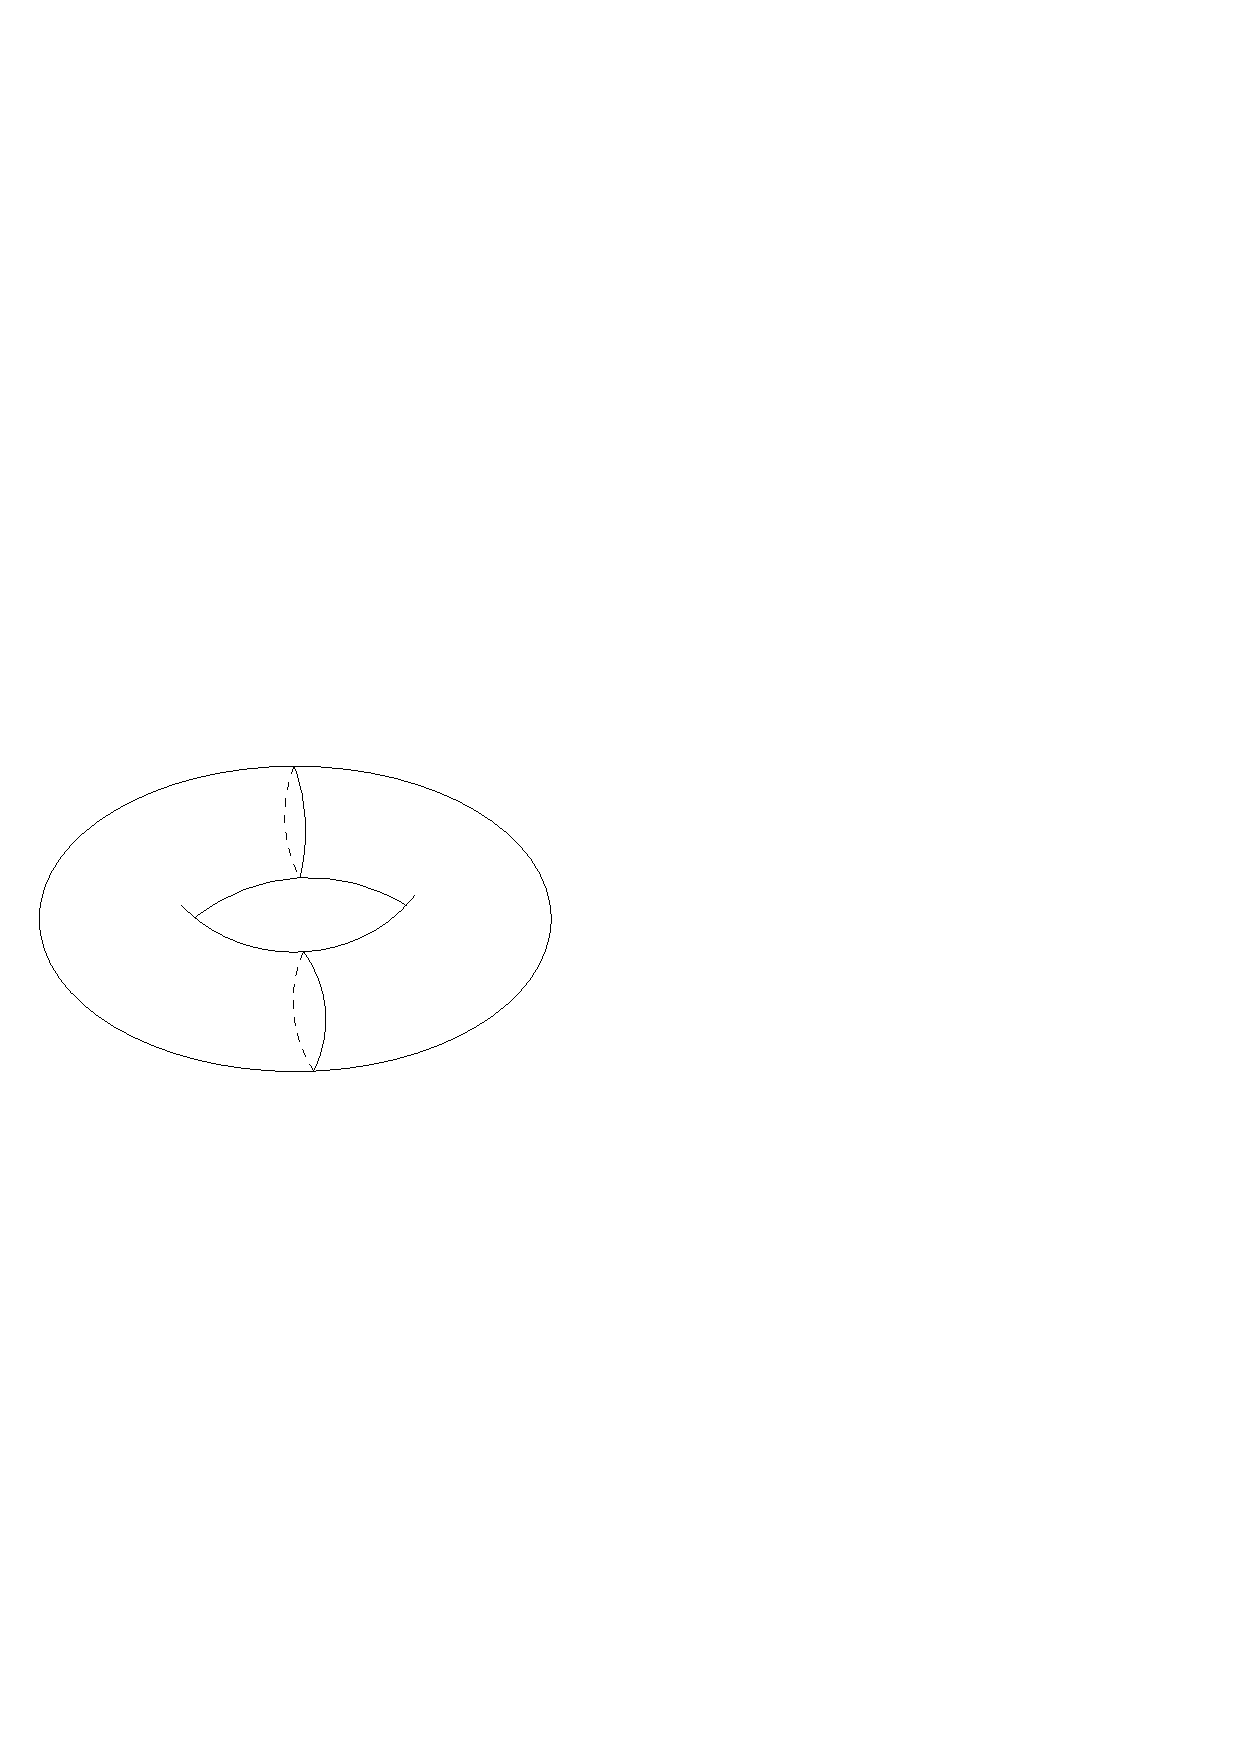
\includegraphics[width=0.5\textwidth]{pictures/cover-by-tori-1}
\caption{The case $n=2k+1$.}
\end{minipage}
\hspace{20pt}
\begin{minipage}{200pt}
\centering
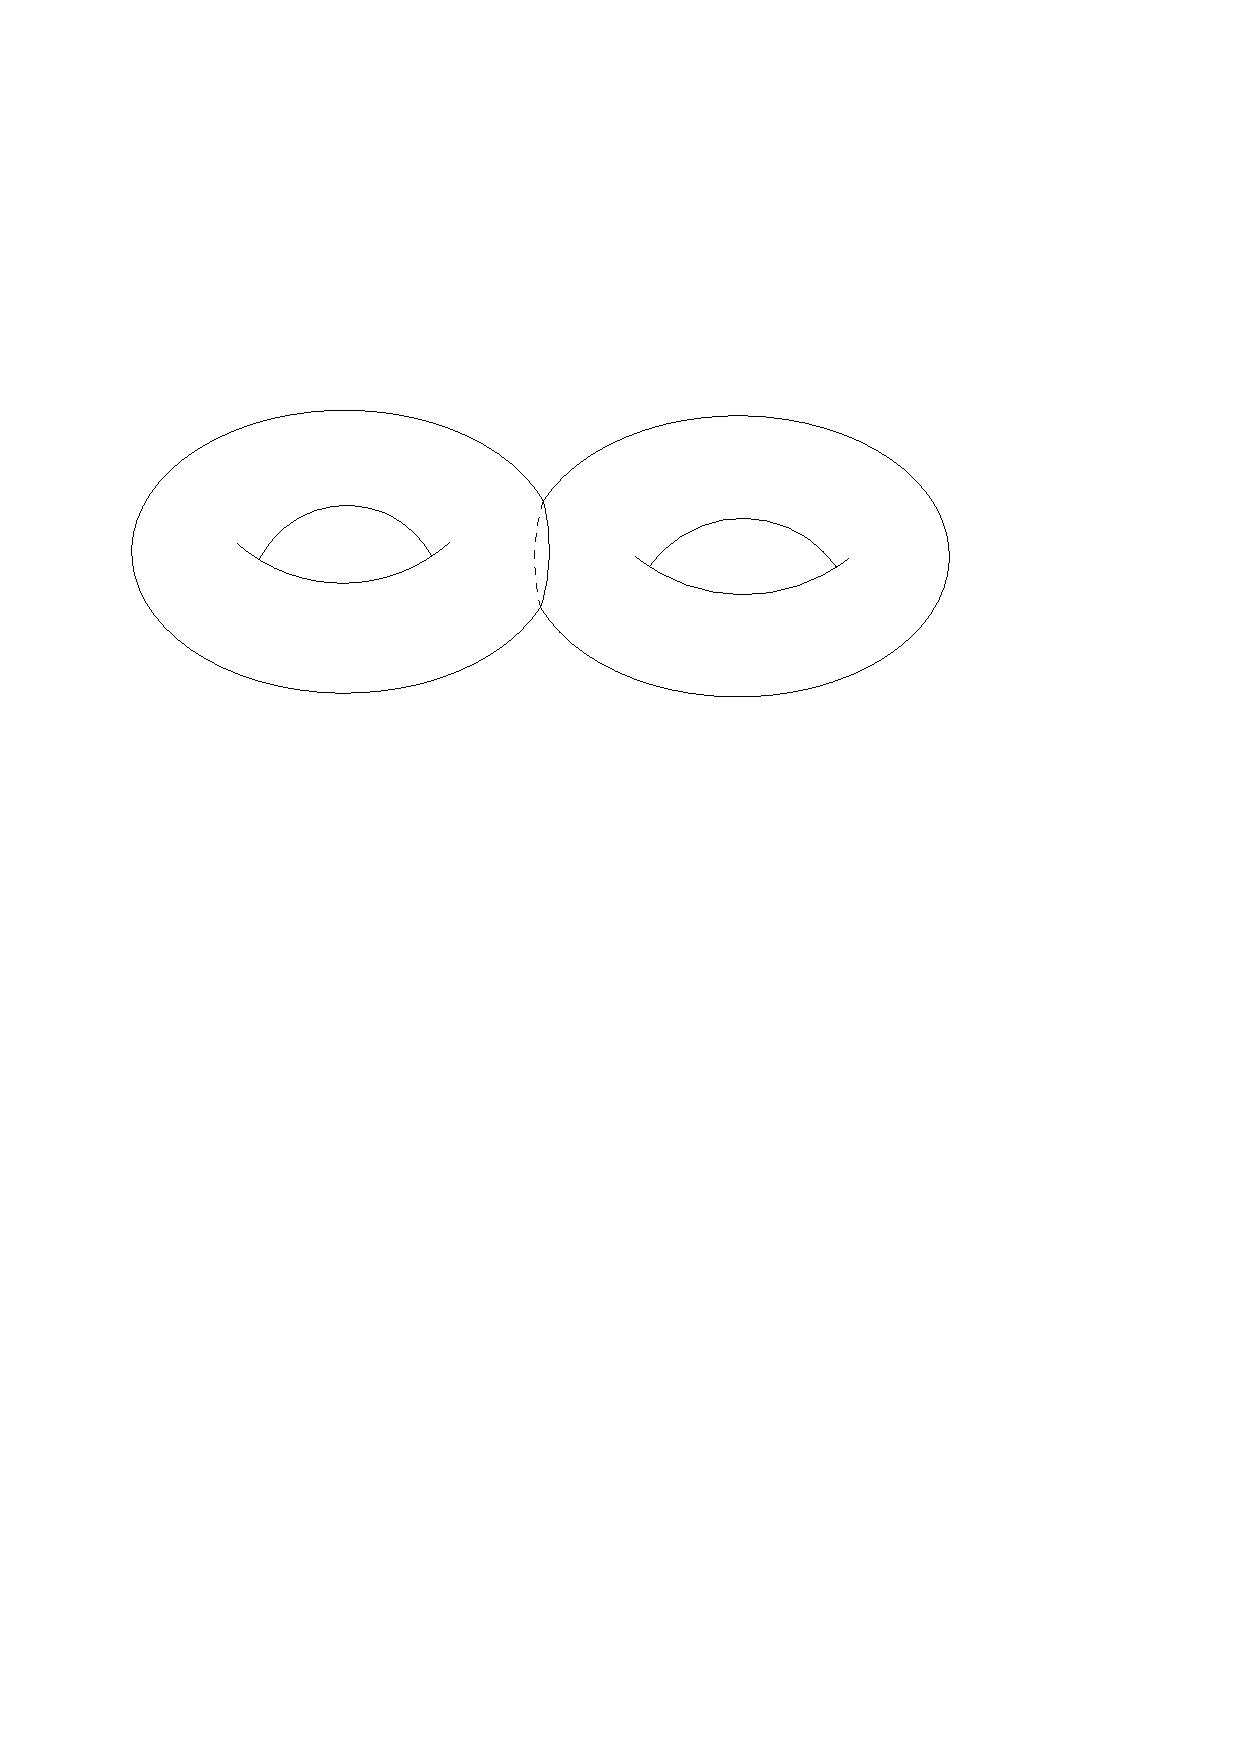
\includegraphics[width=0.8\textwidth]{pictures/cover-by-tori-2}
\caption{The case $n=2k$.}
\end{minipage}
\end{figure}

\end{example}
\begin{exercise}
Let $M$ and $N$ be connected manifolds of dimension $n$, and suppose $p:\widetilde{M}\to M$ is a $k$-sheeted covering map. Show that there is a connected sum $M\#N$ that admits a $k$-sheeted covering by a manifold of the form $\widetilde{M}\#\cdots\#N$ $($connected sum of $\widetilde{M}$ with $k$ disjoint copies of $N$$)$.
\end{exercise}
\begin{proof}
Choose the ball to be cut out of $M$ to lie inside an evenly covered neighborhood
\end{proof}
\begin{exercise}\label{cover map rest}
If $p:E\to X$ is a covering map and $A\sub X$ is a locally path-connected subset, then the restriction of $p$ to each component of $p^{-1}(A)$ is a covering map onto its image.
\end{exercise}
\begin{exercise}
Let $X$ be a CW complex, and let $p:E\to X$ be a covering map. Prove that $E$ has a CW decomposition for which each cell is mapped homeomorphically by $p$ onto a cell 
of $X$.  (Exercise~\ref{cover map rest})
\end{exercise}
\begin{exercise}
Let $p:E\to X$ be a covering map. Show that $E$ is compact if and only if $X$ is compact and $p$ is a finite-sheeted covering.
\end{exercise}
\begin{proof}
If $E$ is compact, then $f(E)=X$ is compact. And each fiber $f^{-1}(y)$ is closed since every point is an isolated point. Thus is compact in $E$. Since $f^{-1}(y)$ is discrete, it is compact if and only if it is finite, so $p$ is a finite-sheeted covering.\par
Assume the condition on $X$ and $p$, from the previous exercise, $p$ is proper, so $p^{-1}(X)=E$ is compact.
\end{proof}
\begin{exercise}
A continuous map $f:S^1\to S^1$ is said to be \textbf{odd} if $f(-z)=-f(z)$ for all $z\in S^1$, and \textbf{even} if $f(-z)=f(z)$ for all $z\in S^1$. Show that every odd map has odd degree.
\end{exercise}
\begin{proof}
Let $\omega$ be the standard generator of $\pi_1(S^1,1)$, so $\omega(s)=e^{2\pi is}$. WLOG we assume $f(1)=1$, so that $f\circ\omega$ is a loop at $1$, and let $\widetilde{f\circ\omega}$ be its lifting. Then be definition we have
\[\deg f=N(f\circ\omega)=\widetilde{f\circ\omega}(1).\]
Let $p:\R\to S^1$ be the covering map, then
\[p\circ\widetilde{f\circ\omega}(\dfrac{1}{2})=f\circ\omega(\dfrac{1}{2})=f(-1)=-1.\]
By the explicit formular $p(x)=e^{2\pi ix}$, we conclude $\widetilde{f\circ\omega}(1/2)=k+1/2$ for some $k\in\Z$. Since $f$ is odd, and observe that $\omega(t+1/2)=-\omega(t)$, we get
\[p\circ\widetilde{f\circ\omega}(t+\dfrac{1}{2})=f\circ\omega(t+\dfrac{1}{2})=f(-\omega(t))=-f\circ\omega(t)=-p\circ\widetilde{f\circ\omega}(t).\]
By the property of $p$, we conclude
\[\widetilde{f\circ\omega}(t+\dfrac{1}{2})-\widetilde{f\circ\omega}(t)\equiv\dfrac{1}{2}\mod\Z.\]
Since the map on the left side is continuous, it must be constant, say $n$. Hence we conclude
\[N(f\circ\omega)=\widetilde{f\circ\omega}(1)-\widetilde{f\circ\omega}(0)=[\widetilde{f\circ\omega}(1)-\widetilde{f\circ\omega}(\dfrac{1}{2})]+[\widetilde{f\circ\omega}(\dfrac{1}{2})-\widetilde{f\circ\omega}(0)]=2n+1.\]
\end{proof}
\begin{exercise}
Show that every even map $f:S^1\to S^1$ has even degree.
\end{exercise}
\begin{proof}
This can be done similarly.
\end{proof}
\begin{exercise}
Show that for any continuous map $F:S^2\to\R^2$, there is a point $x\in S^2$ such that $F(x)=F(-x)$. $($Thus there is always a pair of antipodal points on the earth that have the same temperature and humidity.$)$
\end{exercise}
\begin{proof}
If not, the map $\varphi$:
\[t\mapsto\dfrac{F(t)-F(-t)}{|F(t)-F(-t)|}\]
gives an odd map from $S^2$ to $S^1$, hence we have the composition
\[\begin{tikzcd}
S^1\ar[r,hook]&S^2\ar[r,"\varphi"]&S^1
\end{tikzcd}\]
is an odd map from $S^1$ to $S^1$, hence has odd degree. But since $\pi_1(S^2)=0$, the induced map $\varphi_*$ in $\pi_1(S^1)$ is zero, which is an contradiction.
\end{proof}
\begin{exercise}\label{counter lift crit}
This exercise shows that the hypothesis that $Y$ is locally path-connected cannot be eliminated from the lifting criterion $(Theorem~\ref{lift crit})$. Let $T$ be the topologist's sine curve, and let $Y$ be the union of $T$ with a semicircular arc that intersects $T$ only at $(0,1)$ and $(2/\pi,1)$.
\begin{itemize}
\item[$(a)$] Show that $Y$ is simply connected.
\item[$(b)$] Show that there is a continuous map $f:Y\to S^1$ that has no lift to $\R$.
\end{itemize}
\end{exercise}
\begin{figure}[htbp]
\centering
\begin{minipage}{200pt}
\centering
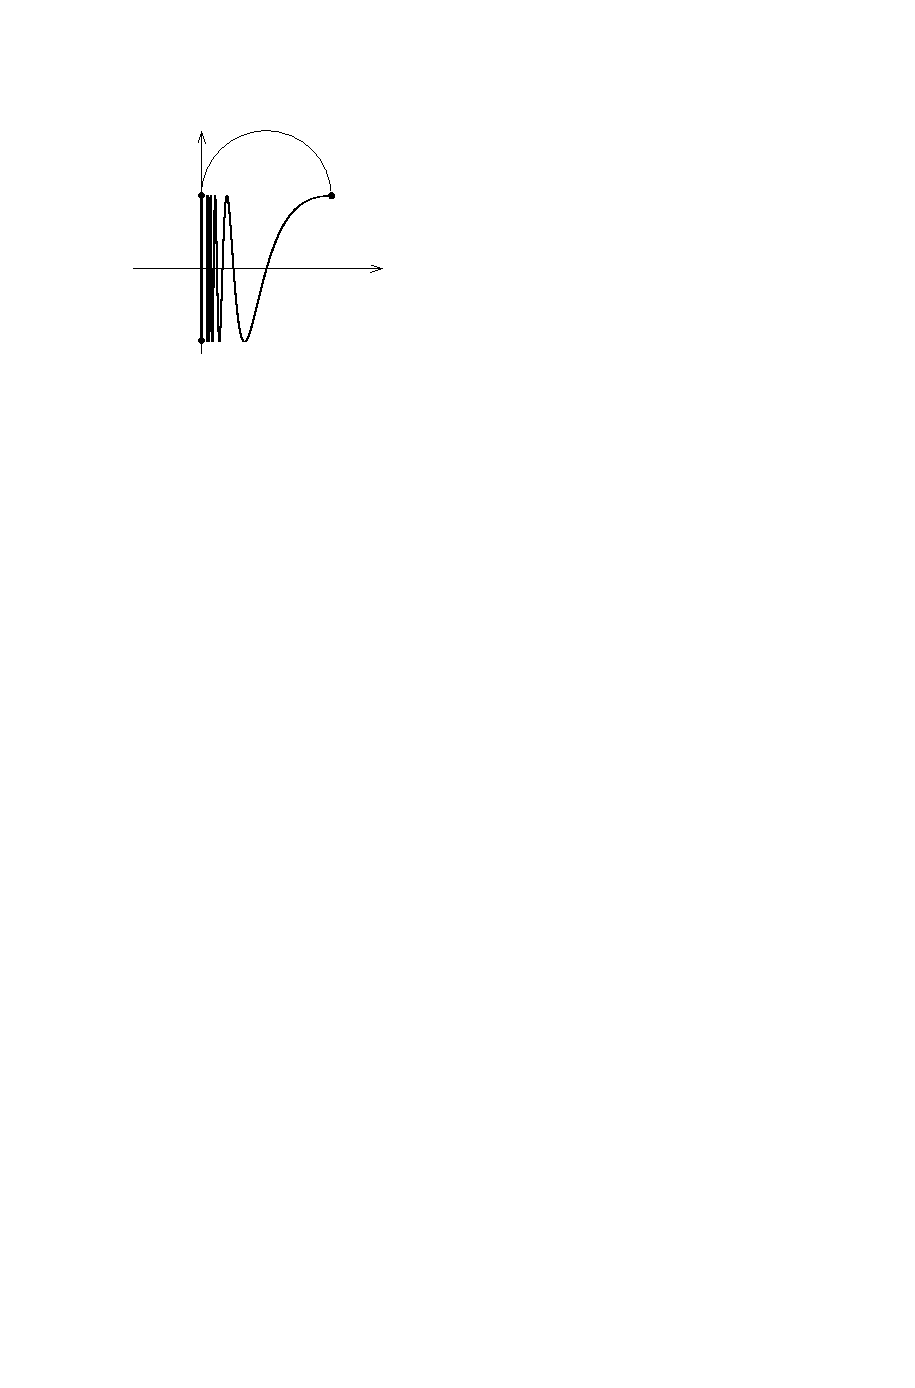
\includegraphics{pictures/sine-curve}
\caption{The space of Exercise~\ref{counter lift crit}.}
\end{minipage}
\hspace{20pt}
\begin{minipage}{200pt}
\centering
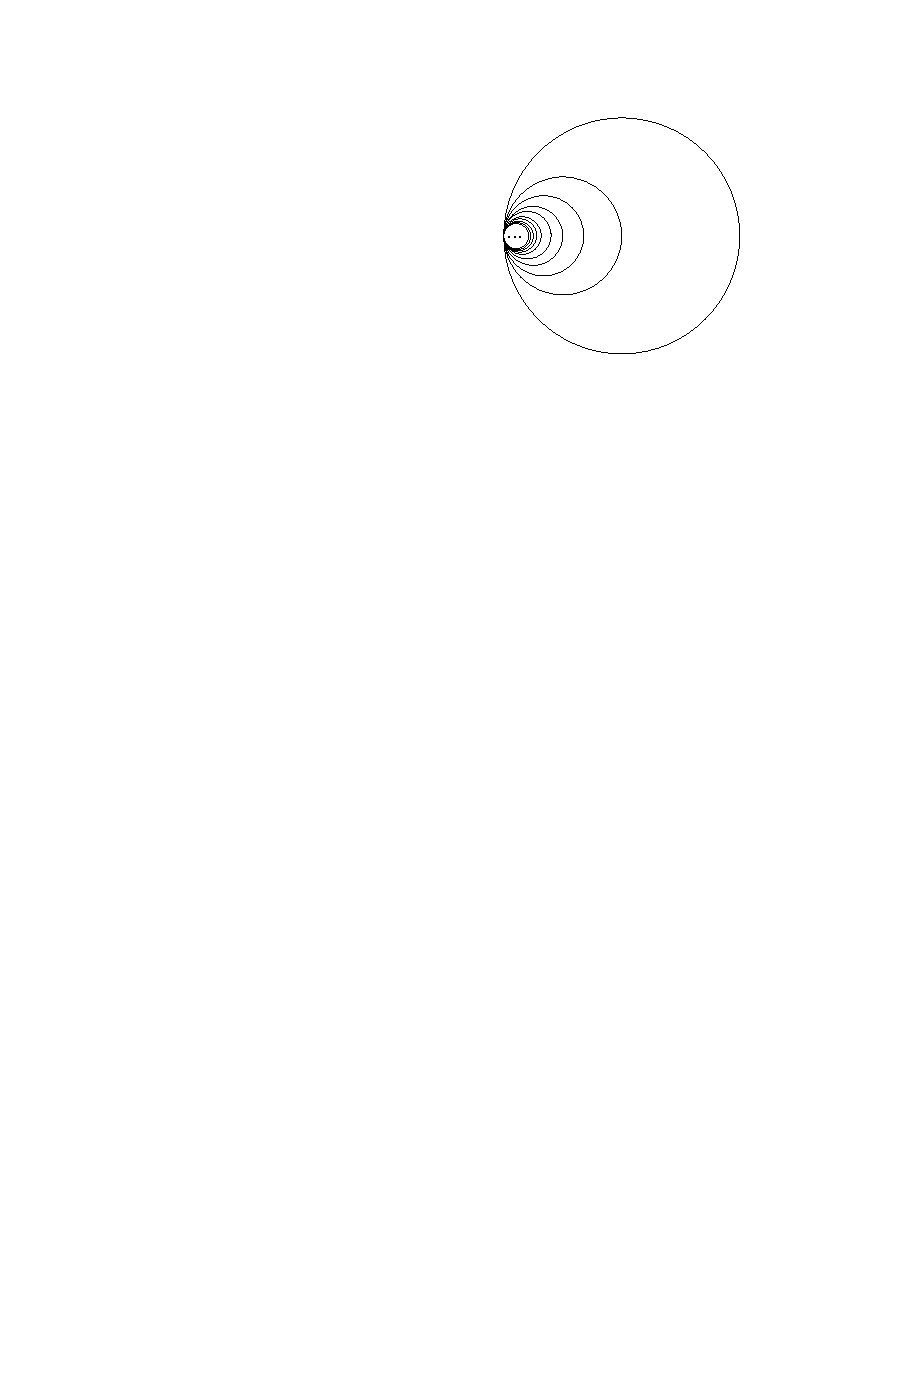
\includegraphics{pictures/Hawaiian-earring}
\caption{The Hawaiian-earring.}
\end{minipage}
\end{figure}
\begin{proof}
The space $T$ is not path connected due to the fact that the point in $L:=\{0\}\times[-1,1]$ has no path-connected neighborhood. Further, any path can not pass $L$ getting into its right part. So the image of any path is contained in a piece of sine curve union the cicluar arc and $L$, which is contractible.\par
Collapsing the interval on $y$-axis into one point, map the sine curve to $I\setminus\{0\}$ and embedd into $S^1$, together with the semicircular arc embedded into $S^1$, we get a map $f:Y\to S^1$ which is continuous. Now assume $\widetilde{f}$ is a lift of $f$, and assume we map $L$ to $1$.\par 
First, note that we warp $Y$ on $S^1$ exactly one round, and $f(Y\setminus L)=S^1\setminus\{1\}$. Since $Y\setminus L$ is connected, so is $\widetilde{f}(Y\setminus L)$. Then $\widetilde{f}(Y\setminus L)$ is contained in one sheet of $p^{-1}(S^1\setminus\{1\})$, which we assume to be $(0,1)$. Since $Y$ is compact, so is $\widetilde{f}(Y)$. In particular, $\widetilde{f}(Y)$ is closed, hence $[0,1]\sub\widetilde{f}(Y)$. But $p\circ \widetilde{f}(L)=f(L)=\{1\}$, so $\widetilde{f}(L)\sub p^{-1}(1)$. And $\widetilde{f}(L)$ is connected, so it must be one point. This is a contradiction because $\{0,1\}\sub\widetilde{f}(L)$.
\end{proof}
\begin{exercise}
For each $n\in\N$, let $C_n$ denote the circle in $\R^2$ with center $(1/n,0)$ and radius $1/n$. The \textbf{Hawaiian earring} is the space $H=\bigcup_{n\in\N}C_n$, with the subspace topology.
\begin{itemize}
\item[$(a)$]Show that $H$ is not semilocally simply connected, and therefore has no universal covering space.
\item[$(b)$]Show that the cone on $H$ is simply connected and semilocally simply connected, but not locally simply connected.
\end{itemize}
\end{exercise}
\begin{proof}
$(a)$ The point $(0,0)$ has no relatively simply connected neighborhood.\par
$(b)$ Any cone $CX$ is contractible, hence simply connected. So semilocally simply connected follows obviously. But there is no simply connected neighborhood for $(0,0)\times I$.
\end{proof}
\begin{exercise}
Suppose $X$ is a connected space that has a contractible universal covering space. For any connected and locally path-connected space $Y$, show that a continuous map $f:Y\to X$ is null-homotopic if and only if for each $y\in Y$, the induced homomorphism $f_*:\pi_1(Y,y)\to\pi_1(X,f(y))$ is the trivial map.
Give a counterexample to show that this result need not hold if the universal covering space is not contractible.
\end{exercise}
\begin{proof}
If $f$ is null-homotopic, by Lemma~\ref{homotopic map incude}, $f_*$ is the trivial map.\par
If $f_*$ is trivial, by the lifting criterion, $f$ has a lifting $\widetilde{f}:Y\to\widetilde{X}$ where $\widetilde{X}$ is the contractible universal covering of $X$. Since $\widetilde{X}$ is contractible, $\widetilde{f}$ is homotopic to a constant map $c$, then $f=p\circ\widetilde{f}\simeq p\circ c$ which is a constant map.\par
$S^2$ is a universal covering of $\P^2$, which is not contractible. Let $Y=S^2$, $f:Y\to\P^2$ be the covering map, then $f_*$ is trivial, and $id_{S^2}$ is a lift of it. But it is not null-homotopic since $S^2$ is not contracible.\par
In fact, if $\widetilde{X}$ is the universal covering of $X$ which is not contractible, take $Y=\widetilde{X}$ gives a counterexample.
\end{proof}
\section{Group Actions and Covering Maps}
In this section, we study the question of \textit{existence} of coverings.\par
\subsection{The Automorphism Group of a Covering}
We begin our exploration of the relationship between group actions and covering spaces by examining a natural group action associated with every covering space.\par
Suppose $p:E\to X$ is a covering map. An \textbf{automorphism of $\bm{p}$} is a covering isomorphism from $p$ to itself, that is, a homeomorphism $\varphi:E\to E$ such that $p\circ\varphi=p$:
\[\begin{tikzcd}
E\ar[rr,"\varphi"]\ar[rd,swap,"p"]&&E\ar[ld,"p"]\\
&X&
\end{tikzcd}\]
Covering automorphisms are also variously known as \textbf{deck transformations} or \textbf{covering transformations}.\par
Let $\Aut_p(E)$ denote the set of all automorphisms of the covering $p:E\to X$. It is easy to verify that $\Aut_p(E)$ is a group, called the \textbf{automorphism group of the covering} (or sometimes the \textbf{covering group}). It acts on $E$ in a natural way, and the definition of covering automorphisms implies that each orbit is a subset of a single fiber.
\begin{proposition}[\textbf{Properties of the Automorphism Group}]\label{auto group prop}
Let $p:E\to X$ be a covering map.
\begin{itemize}
\item[$(a)$]If two automorphisms of $p$ agree at one point, they are identical.
\item[$(b)$]Given $x\in X$, each covering automorphism restricts to a $\pi_1(X,x)$-automorphism of the fiber $p^{-1}(x)$ $($with respect to the monodromy action$)$.
\item[$(c)$]For any evenly covered open subset $U\sub X$, each covering automorphism permutes the components of $p^{-1}(U)$.
\item[$(d)$]The group $\Aut_p(E)$ acts freely on $E$ by homeomorphisms.
\end{itemize}
\end{proposition}
\begin{proof}
Parts $(a)$ and $(b)$ follow immediately from Proposition~\ref{covering homo}$(a,b)$. To prove $(c)$, let $U$ be an evenly covered open subset, and let $U_\alpha$ be a component of $p^{-1}(U_\alpha)$. Since $\varphi(U_\alpha)$ is a connected subset of $p^{-1}(U_\alpha)$, it must be contained in a single component;
applying the same argument to $\varphi^{-1}$ shows that $\varphi(U_\alpha)$ is exactly a component.\par
Finally, to prove $(d)$, just note that the automorphism group acts by homeomorphisms by definition, and the fact that it acts freely follows from $(a)$ by comparing $\varphi$ with the identity.
\end{proof}
\begin{example}
For the covering $p:\R\to S^1$, the integral translations $x\mapsto x+k$ for $k\in\Z$ are easily seen to be automorphisms. To see that every automorphism is of this form, let $\varphi\in\Aut_p(\R)$ be arbitrary. If we set $n=\varphi(0)$, then $\varphi$ and the translation $x\mapsto x+n$ are both covering automorphisms taking $0$ to $n$, so they are equal by Proposition~\ref{auto group prop}$(a)$. Thus the automorphism group of $p:\R\to S^1$ is isomorphic to $\Z$, acting on $\R$ by integral translations. A similar argument shows
that the automorphism group of $p:\R^n\to T^n$ is isomorphic to $\Z^n$ acting by $(x_1,\cdots,x_n)\mapsto(x_1+k_1,\cdots,x_n+k_n)$.
\end{example}
\begin{example}
If $p:S^n\to\P^n$ is the covering map, then the antipodal map $\alpha:S^n\to S^n$ defined by $\alpha(x)=-x$ is an automorphism. The covering automorphism group is the two-element group $\{id,\alpha\}$.
\end{example}
It is important to be aware that, although Proposition~\ref{auto group prop}$(b)$ guarantees that the action of the covering group restricts to an action on each fiber, this action on fibers,
unlike the monodromy action, is not transitive in general. The next theorem gives a criterion for deciding when two points in a fiber are in the same orbit of the covering automorphism group.
\begin{theorem}[\textbf{Orbit Criterion for Covering Automorphisms}]\label{orbit crit auto}
Let $p:E\to X$ be a covering map. If $e_1,e_2\in E$ are two points in the same fiber $p^{-1}(x)$, there exists a covering automorphism taking $e_1$ to $e_2$ if and only if the induced subgroups $p_*(\pi_1(E,e_1))$ and $p_*(\pi_2(E,e_2))$ of $\pi_1(X,x)$ are equal.
\end{theorem}
\begin{proof}
This follows immediately from the covering isomorphism criterion (Theorem~\ref{cover iso crit}).
\end{proof}
One crucial consequence of the orbit criterion is the following alternative characterization
of normal covering maps.
\begin{corollary}[\textbf{Normal Coverings Have Transitive Automorphism Groups}]\label{normal cover iff}
If $p:E\to X$ is a covering map, then $\Aut_p(E)$ acts transitively on each fiber if and only if $p$ is a normal covering.
\end{corollary}
\begin{proof}
Let $p:E\to X$ be a covering map, and let $x$ be an arbitrary point of $X$. By virtue of Proposition~\ref{char nomral cover} and Theorem~\ref{orbit crit auto}, we have the following equivalences:
\begin{align*}
\Aut_p(E)&\text{ acts transitively on }p^{-1}(x)\\
&\iff\text{the subgroups }p_*(\pi_1(E,e))\text{ are the same for all }e\in p^{-1}(x)\\
&\iff p\text{ is a normal covering}.
\end{align*}
So the claim follows.
\end{proof}
The fact that covering automorphisms restrict to $\pi_1(X,x)$-automorphisms of fibers (Proposition~\ref{auto group prop}$(b)$) and the similarity between the orbit criterion for covering automorphisms that we just proved and the orbit criterion for abstract $G$-automorphisms (Proposition~\ref{orbit crit G auto}) suggest that there ought to be a strong connection between the monodromy action and the action of the covering automorphism group on fibers. The next theorem bears this out.
\begin{theorem}\label{cover auto G auto}
Suppose $p:E\to X$ is a covering map and $x$ is any point in $X$. The
restriction map $\varphi\mapsto\varphi|_{p^{-1}(x)}$ is a group isomorphism between $\Aut_p(E)$ and the group $\Aut_{\pi_1(X,x)}\big(p^{-1}(x)\big)$ of $\pi_1(X,x)$-automorphisms of $p^{-1}(x)$.
\end{theorem}
\begin{proof}
Proposition~\ref{auto group prop}$(b)$ shows that each covering automorphism restricts to a $\pi_1(X,x)$-automorphism of $p^{-1}(x)$. Since 
\[(\varphi_1\circ\varphi_2)|_{p^{-1}(x)}=(\varphi_1)|_{p^{-1}(x)}\circ(\varphi_2)|_{p^{-1}(x)},\]
the restriction map is a group homomorphism.\par
Proposition~\ref{auto group prop}$(a)$ shows that two covering automorphisms whose restrictions to $p^{-1}(x)$ agree must be identical, so the restriction homomorphism is injective. To see that it is surjective, suppose $\eta:p^{-1}(x)\to p^{-1}(x)$ is any $\pi_1(X,x)$-automorphism of the fiber. If $e_1$ is any point in $p^{-1}(x)$ and $e_2=\eta(e_1)$, then the orbit criterion for $G$-automorphisms (Proposition~\ref{orbit crit G auto}) shows that the isotropy groups of $e_1$ and $e_2$ are the same. Since these isotropy groups are exactly $p_*(\pi_1(E,e_1))$ and $p_*(\pi_1(E,e_2))$, the orbit criterion for covering automorphisms shows that there exists $\varphi\in\Aut_p(E)$ such that $\varphi(e_1)=e_2$. Then $\eta$ and $\varphi|_{p^{-1}(x)}$ are both $\pi_1(X,x)$-isomorphisms of $p^{-1}(x)$ that agree at one point, so they are equal.
\end{proof}
The next theorem is a central result concerning the relationship between covering spaces and fundamental groups. It gives an explicit formula for the automorphism group of a covering in terms of the fundamental groups of the covering space and the base, and can be used to compute the fundamental groups of certain spaces from properties of their coverings
\begin{theorem}[\textbf{Covering Automorphism Group Structure Theorem}]\label{cover auto structure}
Suppose $p:E\to X$ is a covering map, $e\in E$, and $x=p(e)$. Let $G=\pi_1(X,x)$ and $H=p_*(\pi_1(E,e))\sub\pi_1(X,x)$. For each path class $\gamma\in N_G(H)$ $($the normalizer of $H$ in $G$$)$, there is a unique covering automorphism $\varphi_\gamma\in\Aut_p(E)$ that satisfies $\varphi_\gamma(e)=e\cdot\gamma$. The map $\gamma\mapsto\varphi_\gamma$ is a surjective group homomorphism from $N_G(H)$ to $\Aut_p(E)$ with kernel equal to $H$, so it descends to an isomorphism from $N_G(H)/H$ to $\Aut_p(E)$:
\[\Aut_p(E)\simeq\dfrac{N_{\pi_1(X,x)}\big(p_*(\pi_1(E,e))\big)}{p_*(\pi_1(E,e))}\]
\end{theorem}
\begin{proof}
We have two isomorphisms:
\[N_G(H)/H\stackrel{\sim}{\longrightarrow}\Aut_G\big(p^{-1}(x)\big)\stackrel{\sim}{\longrightarrow}\Aut_p(E)\]
The first isomorphism is induced by the map of Theorem~\ref{char G auto}, which sends an element $\gamma\in N_G(H)$ to the unique $G$-automorphism of $p^{-1}(x)$ taking $e$ to $e\cdot\gamma$; and the second is the inverse of the restriction map $\varphi\mapsto\varphi|_{p^{-1}(x)}$, which is an isomorphism by Theorem~\ref{cover auto G auto}. The map $\gamma\mapsto\varphi_\gamma$ described in the statement of the theorem is exactly the composition of these two maps.
\end{proof}
The most important applications of this theorem occur in the special cases in which $p$ is a normal covering or $E$ is simply connected.
\begin{corollary}[\textbf{Normal Case}]\label{normal cover auto}
If $p:E\to X$ is a normal covering, then for any $x\in X$ and any $e\in p^{-1}(x)$, the map $\gamma\mapsto\varphi_\gamma$ of Theorem~\ref{cover auto structure} induces an isomorphism from $\pi_1(X,x)/p_*(\pi_1(E,e))$ to $\Aut_p(E)$.
\end{corollary}
\begin{corollary}[\textbf{Simply Connected Case}]\label{simply cover auto}
If $p:E\to X$ is a covering map and $E$ is simply connected, then the automorphism group of the covering is isomorphic to the fundamental group of $X$. In fact, for any $x\in X$ and $e\in p^{-1}(x)$, the map $\gamma\mapsto\varphi_\gamma$ of Theorem~\ref{cover auto structure} is an isomorphism from $\pi_1(X,x)$ to $\Aut_p(E)$.
\end{corollary}
\begin{example}
Since the automorphism group of $p:\R\to S^1$ is infinite cyclic and $\R$ is simply connected, Corollary~\ref{simply cover auto} yields another proof that the fundamental group of the circle is infinite cyclic.
\end{example}
\begin{example}
Because the automorphism group of the covering $p:S^n\to\P^n$ is
the two-element group $\{\id,\alpha\}$, Corollary~\ref{simply cover auto} gives another proof that $\pi_1(\P^n)=\Z/2\Z$.
\end{example}
\subsection{Quotients by Group Actions}
The next step in classifying coverings is to start with a space $E$ and develop a technique for constructing spaces covered by $E$.\par
To get an idea how to construct spaces covered by $E$, let us suppose $p:E\to X$ is a normal covering. As Proposition~\ref{auto group prop} showed, the automorphism group $\Aut_p(E)$ acts freely on $E$ by homeomorphisms. Corollary~\ref{normal cover iff} says that $\Aut_p(E)$ acts transitively on each fiber when $p$ is normal, so the identifications made by $p$ are exactly those determined by the equivalence relation $e_1\sim e_2$ if and only if $e_2=\varphi(e_1)$ for some $\varphi\in\Aut_p(E)$. Since $p$ is a quotient map, $X$ is homeomorphic to the orbit space determined by the action of $\Aut_p(E)$ on $E$.\par
Now let $E$ be an arbitrary topological space, and suppose we are given an action by a group $\Gamma$ on $E$. Our aim is to describe conditions under which the quotient map $p:E\to E/\Gamma$ onto the orbit space is a covering map whose automorphism group is $\Gamma$. Note that this construction can produce only normal coverings, because $\Gamma$ acts transitively on
the fibers of any orbit space by definition.\par
Not every group action yields a covering map, of course. Certainly, the group must act freely by homeomorphisms (Proposition~\ref{auto group prop}$(d)$). Moreover, every point of a covering space $E$ has a neighborhood (one of the sheets over an evenly covered open subset) whose images under the automorphism group are all disjoint. This turns out to be the crucial property.\par
Suppose we are given an action by a group $\Gamma$ on a topological space $E$. It is called a \textbf{covering space action} if $\Gamma$ acts by homeomorphisms and every point $e\in E$ has a neighborhood $U$ satisfying the following condition:
\begin{align}\label{covering action-1}
\text{for each }g\in\Gamma, U\cap(g\cdot U)=\emp\text{ unless }g=1.
\end{align}
In fact, any set $U$ satisfying $(\ref{covering action-1})$ satisfies the 
stronger property that all of its images under elements of $\Gamma$ are 
pairwise disjoint: if $g,g'$ are distinct elements of $\Gamma$, then 
$(g\cdot U)\cap(g'\cdot U)=g\cdot(U\cap(g^{-1}g'\cdot U))=\emp$. It is 
immediate from the definition that a covering space action is free.\par
Given an action of a group $\Gamma$ on a space $E$ by homeomorphisms, each 
$g\in\Gamma$ determines a homeomorphism from $E$ to itself by $e\mapsto g\cdot e$. 
We say the action is \textbf{effective} if the map $\Gamma\to\mathrm{Homeo}(E)$ is 
injective. In particular, every free action is effective. If $\Gamma$ acts effectively, it 
is frequently useful to identify $\Gamma$ with the corresponding group of 
homeomorphisms of $E$, and we often do so in this section.
\begin{theorem}[\textbf{Covering Space Quotient Theorem}]\label{cover map iff cover action}
Let $E$ be a connected, locally path-connected space, and suppose we are given an effective action of a group $\Gamma$ on $E$ by homeomorphisms. Then the quotient map $p:E\to E/\Gamma$ is a covering map if and only if the action is a covering space action. In this case, $p$ is a normal covering map, and $\Aut_p(E)=\Gamma$, considered as a group of homeomorphisms of $E$.
\end{theorem}
\begin{proof}
Assume first that $p$ is a covering map. Then the action of each $g\in\Gamma$ is an automorphism of the covering, because it is a homeomorphism satisfying $p(g\cdot e)=p(e)$, so we can identify $\Gamma$ with a subgroup of $\Aut_p(E)$. The action of $\Aut_p(E)$ is a covering space action by Exercise~\ref{cover is cover action}, and the action of $\Gamma$ is too, by Exercise~\ref{cover action rest}.\par
Conversely, suppose the action is a covering space action. Clearly, the quotient 
map $p$ is surjective and continuous. In addition, it is an open map, since for 
each open subset $O\sub E$, $p^{-1}(p(O))$ is the open set
\[p^{-1}(p(O))=\bigcup_{g\in\Gamma}g\cdot O\]
and therefore $p(O)$ is open by the definition of quotient topology. To show that $p$ is a covering map, suppose $x\in E/\Gamma$ is arbitrary. Choose $e\in p^{-1}(x)$, and let $U$ be a neighborhood of $e$ satisfying $(\ref{covering action-1})$. Since $E$ is locally path-connected, by passing to the component of $U$ containing $e$, we can assume that $U$ is path-connected. Let $V=p(U)$, which is a path-connected neighborhood of $x$.\par
Now, $p^{-1}(V)$ is equal to the union of the disjoint connected open subsets $g\cdot U$ for $g\in\Gamma$, so to show that $p$ is a covering it remains only to show that $p$ is a homeomorphism from each such set onto $V$. For each $g\in\Gamma$, the restricted map $g:U\to g\cdot U$ is a homeomorphism, and the diagram
\[\begin{tikzcd}
U\ar[rr,"g"]\ar[rd,swap,"p"]&&g\cdot U\ar[ld,"p"]\\
&V&
\end{tikzcd}\]
commutes; thus it suffices to show that $p|_U:U\to V$ is a homeomorphism. It is surjective, continuous, and open; and it is injective because $p(e)=p(e')$ for $e,e'\in U$ implies $e'=g\cdot e$ for some $g\in\Gamma$, so $e=e'$ because of $(\ref{covering action-1})$. This proves that $p$ is a covering map.\par
To prove the final statement of the theorem, suppose the action is a covering space action. As noted above, each map $e\mapsto g\cdot e$ is a covering automorphism, so $\Gamma\sub\Aut_p(E)$. By construction, $\Gamma$ acts transitively on each fiber, so $\Aut_p(E)$ does too, and thus $p$ is a normal covering. If $\varphi$ is any covering automorphism, choose $e\in E$ and let $e'=\varphi(e)$. Then there is some $g\in\Gamma$ such that $g\cdot e=e'$; since $\varphi$ and $x\mapsto g\cdot x$ are covering automorphisms that agree at a point, they are equal. Thus $\Gamma$ is the full automorphism group.
\end{proof}
A particularly important example of a covering space action arises when we consider a topological group $G$ and a discrete subgroup $\Gamma\sub G$.
\begin{proposition}
Let $\Gamma$ be a discrete subgroup of a connected and locally pathconnected topological group $G$. Then the action of $\Gamma$ on $G$ by right translations is a covering space action, so the quotient map $p:G\to G/\Gamma$ is a normal covering map.
\end{proposition}
\begin{proof}
Because $\Gamma$ is discrete, there is a neighborhood $V$ of $1$ in $G$ 
such that $V\cap\Gamma=\{1\}$. By Lemma~\ref{topo group identity nbhd lem}, 
we can find a neighborhood $U\sub V$ such that $g,h\in U$ implies 
$g^{-1}h\in V$. We complete the proof by showing that $U$ satisfies
$(\ref{covering action-1})$.\par
Suppose $g$ is an element of $\Gamma$ such that $U\cap (U\cdot g)\neq\emp$. 
This means there exists $h\in U$ such that $hg\in U$. By the property of $U$, 
it follows that $g=h^{-1}(hg)\in V\cap\Gamma$, which implies that $g=1$ as 
claimed.
\end{proof}
\begin{corollary}\label{subgroup cover}
Suppose $G$ and $H$ are connected and locally path-connected topological groups, and $\varphi:G\to H$ is a surjective continuous homomorphism with discrete kernel. If $\varphi$ is an open or closed map, then it is a normal covering map.
\end{corollary}
\begin{proof}
Let $\Gamma=\ker\varphi$. By the preceding proposition, the quotient map $p:G\to G/\Gamma$ is a normal covering map. The assumption that $\varphi$ is either open or closed implies that it is a quotient map, and by the first isomorphism theorem the identifications made by $\varphi$ are precisely those made by $p$. Thus the result follows from the uniqueness of quotient spaces.
\end{proof}
\begin{example}\label{torus cover eg-1}
For any integers $a,b,c,d$ such that $ad-bc\neq0$, consider the map $p:T^2\to T^2$ given by $p(z,w)=(z^aw^b,z^cw^d)$. This is easily seen to be a surjective continuous homomorphism, and it is a closed map by
the closed map lemma. Once we show that it has discrete kernel, it follows from the preceding corollary that it is a normal covering map.\par
Let $A$ denote the invertible linear transformation of $\R^2$ whose matrix is 
\[\begin{pmatrix}a&b\\c&d\end{pmatrix}\]
Then we have a commutative diagram
\[\begin{tikzcd}
\R^2\ar[d,swap,"\eps^2"]\ar[r,"A"]&\R^2\ar[d,"\eps^2"]\\
T^2\ar[r,"p"]&T^2
\end{tikzcd}\]
where $\eps^2(x,y)=(e^{2\pi ix},e^{2\pi iy})$ is the universal covering map of the torus. To identify $\ker p$, note that
\begin{align*}
p\circ\eps^2(x,y)=(1,1)&\iff\eps^2\circ A(x,y)=(1,1)\\
&\iff A(x,y)\in\Z^2\\
&\iff (x,y)\in A^{-1}(\Z^2).
\end{align*}
where $A^{-1}(\Z^2)$ denotes the additive subgroup $\{A^{-1}(m,n):(m,n)\in\Z^2\}$ of $\R^2$. Because $\eps^2$ is surjective, this shows that $\ker p=\eps^2\circ A^{-1}(\Z^2)$.\par
Since $A^{-1}$ has rational entries, it follows easily that each element of $\ker p$ is a torsion element of $T^2$. Moreover, since $\Z^2$ is generated $($as a group$)$ by the two elements $(1,0)$ and $(0,1)$, $\ker p$ is generated by their images under $\eps^2\circ A^{-1}$. An abelian group that is generated by finitely many torsion elements is easily seen to be finite; in particular, it is discrete.
\end{example}
\begin{example}\label{torus cover eg-2}
Similar to Example~\ref{torus cover eg-1}, for any integers $a,b,c,d$ such that $ad-bc\neq0$, the map $p:S^1\times\R\to T^2$ given by $p(z,y)=\big(z^a\eps(y)^b,z^c\eps(y)^d\big)$ is a covering map. And we have the following diagram
\[\begin{tikzcd}
\R^2\ar[d,swap,"\eps\times\id_{\R}"]\ar[r,"A"]&\R^2\ar[d,"\eps\times\id_{\R}"]\\
S^1\times\R\ar[d,swap,"\id_{S^1}\times\eps"]\ar[r,"\varphi_A"]&S^1\times\R\ar[d,"\id_{S^1}\times\eps"]\\
T^2\ar[r,"p"]&T^2
\end{tikzcd}\]
where $\varphi_A$ is the induced by $A$ such that the upper rectangle is commutative.
\end{example}
\subsection{The Classification Theorem}
\begin{theorem}[\textbf{Classification of Coverings}]
Let $X$ be a topological space that has a universal covering space, and let $x_0\in X$ be any base point. There is a one-to-one correspondence between isomorphism classes of coverings of $X$ and conjugacy classes of subgroups of $\pi_1(X,x_0)$. The correspondence associates each covering $p:E\to X$ with the conjugacy class of its induced subgroup.
\end{theorem}
\begin{proof}
The covering isomorphism theorem shows that there is at most one isomorphism class of coverings corresponding to any conjugacy class of subgroups, so all we need to show is that there is at least one. Let $H\sub\pi_1(X,x_0)$ be any subgroup in the given conjugacy class. Let $p:E\to X$ be the universal covering of $X$, and choose a base point $e_0\in E$ such that $p(e_0)=x_0$. Then the simply connected case of the automorphism group structure theorem (Corollary~\ref{simply cover auto}) shows that $\pi_1(X,x_0)$ is isomorphic to the automorphism group $\Aut_p(E)$, under the map that sends each path class $\gamma\in\pi_1(X,x_0)$ to the unique automorphism $\varphi_\gamma\in\Aut_p(E)$ that satisfies $\varphi_\gamma(e_0)=e_0\cdot\gamma$. Let $\widehat{H}\sub\Aut_p(E)$ be the image of $H$ under this isomorphism, so $\widehat{H}=\{\varphi_\gamma:\gamma\in H\}$.\par
Since the action of $\Aut_p(E)$ on $E$ is a covering space action, it follows from Exercise~\ref{cover action rest} that the restriction of the action to $\widehat{H}$ is too. Let $E$ denote the quotient
space $E/\widehat{H}$ and $Q:E\to E/\widehat{H}$ the quotient map; by Theorem~\ref{cover map iff cover action}, $Q$ is a normal covering map and $\widehat{H}=\Aut_Q(E)$. Moreover, $p:E\to X$ is constant on the fibers of $Q$ (because they are contained in the fibers of $p$), so $p$ descends to a continuous map $\widehat{p}:\widehat{E}\to X$ such that the following diagram commutes:
\[\begin{tikzcd}
E\ar[dd,"p"]\ar[rd,"Q"]&\\
&\widehat{E}\ar[ld,"\widehat{p}"]\\
X
\end{tikzcd}\]
We have to show that $\widehat{p}$ is a covering map. Let $x\in X$ be arbitrary, and let $U$ be a neighborhood of $x$ that is evenly covered by $p$. We will show that $U$ is also evenly covered by $\widehat{p}$. Given a component $U_i$ of $p^{-1}(U)$, let $\widehat{U}_i=Q(U_i)\sub\widehat{E}$; then $\widehat{U}_i$ is connected, and it is open in $\widehat{E}$ because $Q$ is an open
map. Suppose $\widehat{U}_i=Q(U_i)$ and $\widehat{U}_j=Q(U_j)$ are any two such sets. If they have a point $\widehat{e}$ in common, then $\widehat{e}=Q(e_i)=Q(e_j)$ for some $e_i\in U_i$ and $e_j\in U_j$. Since $Q$ identifies points of $E$ if and only if they are in the same $\widehat{H}$-orbit, there is some $\varphi\in\widehat{H}$ such that $e_j=\varphi(e_i)$. Then $\varphi(U_i)=U_j$ by Proposition~\ref{auto group prop}$(c)$, so $Q(U_i)=Q\circ\varphi(U_i)=U_j$. This shows that any such sets $\widehat{U}_i,\widehat{U}_j$ are either disjoint or equal. Since $Q$ is surjective, $\widehat{p}^{-1}(U)$ is equal to the disjoint union of the connected open sets $\widehat{U}_i$ as $U_i$ ranges over the components of $p^{-1}(U)$.\par 
It remains only to show that for any such set $\widehat{U}_i$, the restricted map $\widehat{p}:U_i\to U$ is a homeomorphism. The following diagram commutes:
\[\begin{tikzcd}
U_i\ar[dd,"p"]\ar[rd,"Q"]&\\
&\widehat{U}_i\ar[ld,"\widehat{p}"]\\
U&
\end{tikzcd}\]
Since $p=\widehat{p}\circ Q$ is injective on $U_i$, so is $Q$; and $Q:U_i\to\widehat{U}_i$ is surjective by definition. Because $Q$ is an open map, it follows that $Q:U_i\to\widehat{U}_i$ is a homeomorphism. Since $p$ and $Q$ are homeomorphisms, so is $\widehat{p}$.\par
The last step is to show that $\widehat{p}(\pi_1(\widehat{E},\widehat{e}_0))=H$ for some $\widehat{e}_0\in\widehat{E}$ such that $\widehat{p}(\widehat{e}_0)=x_0$. Choose $\widehat{e}_0=Q(e_0)$. By Theorem~\ref{iso group of monodromy}, $\widehat{p}(\pi_1(\widehat{E},\widehat{e}_0))$ is the isotropy group of $\widehat{e}_0$ under the monodromy action by $\pi_1(X,x_0)$ on $\widehat{E}$. Suppose $\gamma\in\pi_1(X,x_0)$ is arbitrary. Since $Q$ restricts to a $\pi_1(X,x_0)$-equivariant map from $p^{-1}(x_0)$ to $\widehat{p}^{-1}(x_0)$ by Proposition~\ref{covering homo}$(b)$, we have
\[\widehat{e}_0\cdot\gamma=Q(e_0)\cdot\gamma=Q(e_0\cdot\gamma)=Q(\varphi_\gamma(e_0)).\]
Since $\widehat{e}_0=Q(e_0)$, it follows that $\gamma$ is in the isotropy group of $\widehat{e}_0$ if and only if $Q(\varphi_\gamma(e_0))=Q(e_0)$, which is the case if and only if $\varphi_\gamma\in\widehat{H}$, which in turn is true if and only if $\gamma\in H$.
\end{proof}
The proof of the theorem yields the following useful explicit description of the covering associated with a particular subgroup of the fundamental group.
\begin{corollary}
Suppose $p:E\to X$ is the universal covering of a space $X$, and $x_0\in X$ is any base point. Given a subgroup $H\sub\pi_1(X,x_0)$, let $\widehat{H}\sub\Aut_p(E)$ be
the subgroup corresponding to $H$ under the isomorphism of Corollary~\ref{simply cover auto}. Then $p$ descends to a continuous map $\widehat{p}:\widehat{E}\to X$, which is a covering map whose induced subgroup is $H$.
\end{corollary}
As an application, we can classify all coverings of the torus.
\begin{proposition}[\textbf{Classification of Torus Coverings}]
Every covering of $T^2$ is isomorphic to precisely one of the following:
\begin{itemize}
\item[$(a)$] The universal covering $\eps^2:\R^2\to T^2$.
\item[$(b)$] A covering $p:S^1\times\R\to T^2$ by $p(z,y)=\big(z^a\eps(y)^b,z^b\eps(y)^{-a}\big)$, where $(a,b)$ is a pair of integers with $a\geq0$ and $b>0$ if $a=0$.
\item[$(c)$] A covering $p:T^2\to T^2$ by $p(z,w)=(z^aw^b,w^c)$, where $(a,b,c)$ are integers with $a>b\geq0$ and $c>0$.
\end{itemize}
\end{proposition}
\begin{proof}
Note that all of these maps are coverings: the universal covering, the maps in part $(b)$ by Example~\ref{torus cover eg-1}, and those in part $(c)$ by Example~\ref{torus cover eg-2}.\par
Let us use $p=(1,1)\in T^2$ as base point, and use the presentation $\pi_1(T^2,p)=\langle\beta,\gamma\mid\beta\gamma=\gamma\beta\rangle$ where $\beta$ and $\gamma$ are the path classes of the standard generator of $\pi_1(S^1,1)$ in the first and second factors, respectively. Then the map $(m,n)\mapsto\beta^m\gamma^n$ is an isomorphism of $\Z^2$ with $\pi_1(T^2,p)$.\par 
The classification theorem says that isomorphism classes of coverings of $T^2$ are in one-to-one correspondence with subgroups of $\pi_1(T^2,p)$ under the correspondence that matches a covering $p:X\to T^2$ with the subgroup induced by $p$. (Since the fundamental group is abelian, each conjugacy class contains exactly one subgroup.) So we begin by showing that each subgroup of $\Z^2$ is one and only one of the following:
\begin{itemize}
\item[$(\rmnum{1})$] The trivial subgroup
\item[$(\rmnum{2})$] An infinite cyclic subgroup generated by $(a,b)$ such that $a\geq0$ and $b>0$ if $a=0$
\item[$(\rmnum{3})$] A subgroup $\langle(a,0),(b,c)\rangle$ generated by two elements $(a,0)$ and $(b,c)$ satisfying $a>b\geq0$ and $c>0$
\end{itemize}
To prove this, let $G$ be an arbitrary subgroup of $\Z^2$. Because $\Z^2$ is free abelian of rank $2$, $G$ is free abelian of rank at most $2$. Thus there are
three mutually exclusive cases, in which $G$ has rank $0$, $1$, or $2$. Clearly, the trivial subgroup has rank $0$; we will show that the rank $1$ and $2$ cases correspond to $(\rmnum{2})$ and $(\rmnum{3})$, respectively.\par
If $G$ has rank $1$, it is cyclic. In this case there are two elements $(a,b)$ and $(-a,-b)$ that generate $G$, and exactly one of these satisfies the conditions of $(\rmnum{2})$. Thus $(\rmnum{2})$ corresponds to the rank $1$ case.\par
It remains to show that when $G$ has rank $2$ there are unique integers $a,b,c$ satisfying the conditions in $(\rmnum{3})$ such that $\{(a,0),(b,c)\}$ forms a basis for $G$. The subgroup $G_1=G\cap(\Z\times\{0\})$ is not trivial: if $\{(m,n),(i,j)\}$ is any basis for $G$, then $j(m,n)-n(i,j)$ is an element of $G$ in $\Z\times\{0\}$, which is not $(0,0)$ because of the independence of $(m,n)$ and $(i,j)$. Since $\Z\times\{0\}$ is cyclic, so is $G_1$. Let $(a,0)$ be a generator of $G_1$; replacing it by its negative if necessary, we may assume $a>0$. Since $G$ has rank $2$, it is not contained in $G_1$. There is a basis for $G$ of the form $\{(a,0),(b,c)\}$, where $c$ is a generator of the image of $G$ under the projection $\pi:\Z^2\to\Z$. Replacing $(b,c)$ by its negative if necessary, we may assume $c>0$. Subtracting a multiple of $(a,0)$ from $(b,c)$ (which still yields a basis), we may assume $a>b\geq0$. Thus we have found $a,b,c$ satisfying the conditions in $(\rmnum{3})$ such that $(a,0)$ and $(b,c)$ are a basis for $G$.\par
Finally, we need to show that two such triples $a,b,c$ and $a',b',c'$ that determine the same subgroup are identical. Since each basis can be expressed in terms
the other, there is an integer matrix $M$ such that
\[\begin{pmatrix}
a&b\\0&c
\end{pmatrix}M=\begin{pmatrix}a'&b'\\0&c'
\end{pmatrix}\]
Examining the lower left entry in this equation shows that $M$ is also upper triangular. Since $M$ has an inverse that also has integer entries, its determinant must be $\pm1$; and then the above equation shows that $\det M=1$ (recall that $a$, $c$, $a'$, and $c'$ are all positive). Since $M$ is upper triangular, its determinant is the product of its (integer) diagonal entries, so these must be both $+1$ or both $-1$; and then the fact that $a$ and $a'$ are both positive forces both diagonal entries to be $1$, so $a=a'$ and $c=c'$. The upper right entry of the matrix equation then becomes $ak+b=b'$ (where $k$ is the upper right entry of $M$). Since $a>b\geq0$ and $a>b'\geq0$, this forces $k=0$, so $M$ is the identity.\par
To complete the proof, we need to check that the subgroups of $\pi_1(T^2,p)$ induced by the covering maps $(a)$, $(b)$, $(c)$ are exactly those corresponding to $(\rmnum{1})$, $(\rmnum{2})$, $(\rmnum{3})$, respectively.\par
Case $(a)$ is immediate, since the fundamental group of $\R^2$ is trivial.\par
For $(b)$, note that the fundamental group of $S^1\times\R$ is infinite cyclic, generated by the path class of the loop $c(t)=(\omega(t),0)$. The image of this loop under $p$ is $p\circ c(t)=(\omega(t)^a,\omega(t)^b)$, which represents the element $\beta^a\gamma^b\in\pi_1(T^2,p)$. Under our isomorphism with $\Z^2$, this corresponds to $(a,b)$ and generates the infinite cyclic group described in $(\rmnum{2})$.\par
For $(c)$, the covering map $p$ carries the generators $\beta$ and $\gamma$ of $\pi_1(T^2,p)$ to $\beta^a$ and $\beta^b\gamma^c$. Under our isomorphism with $\Z^2$, the subgroup generated by these elements is exactly the one described in $(\rmnum{3})$.
\end{proof}
\subsection{Proper Group Actions}
In this subsection we consider the covering map between manifolds. Especially we would like to find conditions on the group action such that the orbit space is a manifold. For this, we first note the following observation.
\begin{theorem}\label{cover mani}
Suppose $p:E\to X$ is a covering map.
\begin{itemize}
\item[$(a)$]If $X$ is Hausdorff, then $E$ is too.
\item[$(b)$]If $X$ is an $n$-manifold, then $E$ is too.
\item[$(c)$]If $E$ is an $n$-manifold, then $X$ is an $n$-manifold if and only if $X$ is Hausdorff.
\end{itemize}
\end{theorem}
\begin{proof}
$(a)$ Let $e_1,e_2$ be distince points in $E$. If $e_1$ and $e_2$ are in the same fiber, the claim is obvious. If they are not, choose disjoint neighborhood of $p(e_1)$, $p(e_2)$, then their preimage under $p$ satisfies the condition.\par
$(b)$ For each point $e\in E$, $p(e)$ has a neighborhood of coordinate ball, let $V$ be the component of the preimage of this ball which contains $e$, then $V$ is a coordinate ball of $e$. Thus $E$ is locally Euclidean.\par 
Now to proof $E$ is second countable, we choose a countable basis $\mathcal{B}$ of $X$ consists of evenly covered coordinate balls. Since the fundamental group of a manifold is countable and the fundamental group acts transitively on the fiber of a point, it follows that the fiber of each point is countable. Thus the collection $p^{-1}(\mathcal{B})$ is also countable. Now $p^{-1}(\mathcal{B})$ covers $E$ and each element in it is homeomorphic to a coordinate ball, hence second countable, it follows that $E$ is second countable.\par
$(c)$ Similar to $(b)$ we can show $X$ is locally Euclidean. Since $p$ is an open map, it take a countable basis from $E$ to $X$, so $X$ is second countable. Now the claim is obvious.
\end{proof}
Given a covering space action of a group $\Gamma$ on a manifold $M$, by 
Theorem~\ref{cover mani}, the orbit space $M/\Gamma$ will be manifold if and only if it is 
Hausdorff. But the Hausdorff condition is not automatic, thus we need to place an extra 
restriction on the action in order to ensure that we will obtain a Hausdorff quotient.\par
One straightforward criterion is the following.
\begin{proposition}[\textbf{Hausdorff Criterion for Orbit Spaces}]
Suppose $E$ is a topological space and $\Gamma$ is a group acting $E$ by homeomorphisms. Then $E/\Gamma$ is Hausdorff if and ony if the action satisfies the following condition:
\begin{equation*}
\parbox{\dimexpr\linewidth-6em}
{\strut
If $e,e'\in E$ lie in different orbits, there exist neighborhoods
$V$ of $e$ and $V'$ of $e'$ such that $V\cap(g\cdot V')=\emp$ for all $g\in\Gamma$.
\strut}
\end{equation*}
Let $\mathcal{O}\sub E\times E$ be the \textbf{orbit relation} defined by
\[\mathcal{O}=\{(e,e'):e'=g\cdot e\text{ for some }g\in\Gamma\}\]
Then this condition is equivalent to that $\mathcal{O}$ is closed in $E\times E$.
\end{proposition}
\begin{proof}
Let $p:E\to E/\Gamma$ denote the quotient map. If $E/\Gamma$ is Hausdorff, then given $e,e'$ in different orbits, there are disjoint neighborhoods $U$ of $p(e)$ and $U'$ of $p(e')$, and then $V=p^{-1}(U)$ and $V'=p^{-1}(U')$ satisfy the condition.\par
Conversely, suppose the action satisfies the condition. Given distinct points $x,x'\in E/\Gamma$, choose $e,e'\in E$ such that $p(e)=x$ and $p(e')=x'$, and let $V,V'$ be neighborhoods satisfying the condition. Because $p$ is an open map, $p(V)$ and $p(V)$ are neighborhoods of $x$ and $x'$, respectively; and they are disjoint.
\end{proof}
A continuous action of a topological group $G$ on a topological space $E$ is 
said to be a \textbf{proper action} if the continuous map $\varTheta:G\times E\to E\times E$ 
defined by
\begin{equation}\label{proper action def}
\varTheta(g,e)=(g\cdot e,e)
\end{equation}
is a proper map. It should be noted that this is a weaker condition than requiring the map 
$G\times E\to E$ defining the group action to be a proper map.\par
The most significant fact about proper actions is that for sufficiently nice spaces, they 
always yield Hausdorff quotients, as the next proposition shows.
\begin{proposition}\label{proper action Hausdorff}
If a topological group $G$ acts continuously and properly on a locally compact Hausdorff space $E$, then the orbit space $E/G$ is Hausdorff.
\end{proposition}
\begin{proof}
Let $\mathcal{O}\sub E\times E$ be the orbit relation. The orbit space is Hausdorff if and only if $\mathcal{O}$ is closed in $E\times E$. But $\mathcal{O}$ is just the image of the map $\varTheta:G\times E\to E\times E$ defined by $(\ref{proper action def})$. Since $E$ is a locally compact Hausdorff space, the same is true of $E\times E$, so it is compactly generated, and it follows that $\varTheta$ is a closed map. Thus the orbit relation is closed and $E/G$ is Hausdorff.
\end{proof}
With this in mind, we now turn our attention to proper actions. First of all, here is a 
useful characterization of proper action.
\begin{proposition}\label{proper action iff}
Suppose we are given a continuous action of a topological group $G$ on a Hausdorff space $E$. The action is proper if and only if for every compact subset $K\sub E$, the set $G_K=\{g\in G:(g\cdot K)\cap K\neq\emp\}$ is compact.
\end{proposition}
\begin{proof}
Let $\varTheta:G\times E\to E\times E$ be the map defined by $(\ref{proper action def})$. Suppose first that $\varTheta$ is proper. Then for any compact set $K\sub E$, we have
\begin{equation}\label{proper action iff-1}
\begin{aligned}
G_K&=\{g\in G:\text{ there exists }e\in K\text{ such that }g\cdot e\in K\}\\
&=\{g\in G:\text{ there exists }e\in K\text{ such that }\varTheta(g,e)\in K\times K\}\\
&=\pi_G\big(\varTheta^{-1}(K\times K)\big)
\end{aligned}
\end{equation}
where $\pi_G:G\times E\to G$ is the projection. Thus $G_K$ is compact.\par
Conversely, suppose $G_K$ is compact for every compact set $K\sub E$. Given a compact subset $L\sub E\times E$, let $K=\pi_1(L)\cup\pi_2(L)\sub E$, where $\pi_1,\pi_2:E\times E\to E$ are the projections onto the first and second factors, respectively. Then
\[\varTheta^{-1}(L)\sub\varTheta^{-1}(K\times K)\sub\pi_G^{-1}(G_K)\]
Since $E\times E$ is Hausdorff, $L$ is closed in $E\times E$, and so $\varTheta^{-1}(L)$ is closed in $G\times E$ by continuity. Thus $\varTheta^{-1}(L)$ is a closed subset of the compact set $G_K\times K$ and is therefore compact.
\end{proof}
\begin{corollary}
Every continuous action of a compact topological group on a Hausdorff space is proper.
\end{corollary}
For sufficiently nice spaces, including all connected manifolds, the next theorem shows that once we know an action is continuous, proper, and free, it is not necessary to check that it is a covering space action.
\begin{theorem}
Suppose $E$ is a connected, locally path-connected, and locally compact Hausdorff space, and a discrete group $\Gamma$ acts continuously, freely, and properly on $E$. Then the action is a covering space action, $E/\Gamma$ is Hausdorff, and the quotient map $p:E\to E/\Gamma$ is a normal covering map.
\end{theorem}
\begin{proof}
We need only show that the action is a covering space action, for then Proposition~\ref{proper action Hausdorff} shows that $E/\Gamma$ is Hausdorff, and the covering space quotient theorem shows that $p$ is a normal covering map.\par
Suppose $e_0\in E$ is arbitrary. Because $E$ is locally compact, $e_0$ has a neighborhood $V$ contained in a compact set $K$. By Proposition~\ref{proper action iff}, the set $\Gamma_K=\{g\in\Gamma:(g\cdot K)\cap K\neq\emp\}$ is compact. Because $\Gamma$ has the discrete topology, this means $\Gamma_K$ is finite; let us write $\Gamma_K=\{1,g_1,\cdots,g_m\}$. Since the action is free and $E$ is Hausdorff, for each $g_i$ there are disjoint neighborhoods $W_i$ of $e_0$ and $W'_i$ of $g_i\cdot e_0$. Let
\[U=V\cap W_1\cap(g_1^{-1}\cdot W'_1)\cap\cdots\cap W_m\cap(g_m^{-1}\cdot W'_m).\]
We will show that $U$ satisfies $(\ref{covering action-1})$.\par
First consider $g=g_i$ for some $i$. If $e\in U\sub g_i^{-1}\cdot W'_i$, then $g_i\cdot e\in W'_i$, which is disjoint from $W_i$ and therefore from $U$. Thus $U\cap(g_i\cdot U)=\emp$. On the other hand, if $g\in\Gamma$ is not the identity and not one of the $g_i$'s, then for any $e\in U\sub V\sub K$, we have $g\cdot e\in g\cdot K$, which is disjoint from $K$ and therefore also from $U$. Thus once
again we have $U\cap(g\cdot U)=\emp$.
\end{proof}
\begin{corollary}
Let $M$ be a connected $n$-manifold on which a discrete group $\Gamma$ acts continuously, freely, and properly. Then $M/\Gamma$ is an $n$-manifold.
\end{corollary}
Now we give an example of our previous results.
\begin{example}[\textbf{Lens Spaces}]
By identifying $\R^4$ with $\C^2$ in the usual way, we can consider $S^3$ as the following subset of $\C^2$:
\[S^3=\{(z_1,z_2)\in\C^2:|z_1|^2+|z_2|^2=1\}.\]
Fix a pair of relatively prime integers $1\leq m<n$, and define an action of $\Z/n\Z$ on $S^3$ by
\[[k]\cdot(z_1,z_2):=(e^{2\pi ik/n}z_1,e^{2\pi ikm/n}z_2)\]
It can easily be checked that this action is free, and it is proper because $\Z/n\Z$ is a finite group.\par
The orbit space $S^3/(\Z/n\Z)$ is thus a compact $3$-manifold whose universal covering space is $S^3$ and whose fundamental group is isomorphic to $\Z/n\Z$. This manifold, denoted by $L(n,m)$, is called a \textbf{lens space}.\par
By the classification theorem, the coverings of $L(n,m)$ are in one-to-one correspondence with subgroups of $\Z/n\Z$. Since every subgroup of a cyclic group is
cyclic, the only possibilities for subgroups $G\sub\pi_1(L(n,m))$ are
cyclic groups of order $p$ where $p$ is a factor of $n$. In each such case, a covering of $L(n,m)$ is obtained by restricting the action of $\Z/n\Z$ on $S^3$ to $G$, and mapping the resulting quotient space down to $L(n,m)$ by sending each $G$-equivalence class to its $\Z/n\Z$-equivalence class. If $n=pq$ for positive integers $p$ and $q$, let $G\sub\Z/n\Z$ be
the cyclic subgroup of order $p$ generated by $($the coset of$)$ $q$. It is easy to check from the definitions that $S^3/G=L(p,m)$, and we obtain a $q$-sheeted covering $L(p,m)\to L(n,m)$. These are the only coverings of the lens spaces up to isomorphism.
\end{example}
\subsection{Application: Universal Coverings of Surfaces}
\begin{theorem}
Let $M$ be a compact surface. The universal covering space of $M$ is homeomorphic to
\begin{itemize}
\item[$(a)$] $S^2$ if $M\approx S^2$ or $\P^2$.
\item[$(b)$] $\R^2$ if $M\approx T^2$ or $\P^2\#\P^2$.
\item[$(c)$] $\B^2$ if $M$ is any other surface.
\end{itemize}
\end{theorem}
\begin{proof}
Because $S^2$ is simply connected, it is its own universal covering space. The universal covering space of $T^2$ is $\R^2$, and that
of $\P^2$ is $S^2$. If $M$ is a connected sum of $n\geq2$ projective planes, then by the result of Exercise~\ref{tori cover proj}, $M$ has a two-sheeted covering by a manifold $N$, which is a connected sum of $n-1$ tori. If $\widetilde{M}$ is the universal covering space of $M$, then $\widetilde{M}$ also covers $N$ by Proposition~\ref{universal cover prop}$(a)$, so $M$ and $N$ have the same universal covering space. Thus to complete the proof of the theorem, it suffices to show that every connected sum of $n\geq 2$ tori is covered by $\B^2$.
\end{proof}
\subsection{Exercise}
\begin{exercise}\label{cover is cover action}
Show that for any covering map $p:E\to X$, the action of $\Aut_p(E)$ on $E$ is a covering space action.
\end{exercise}
\begin{exercise}\label{cover action rest}
Given a covering space action of a group $\Gamma$ on a topological space $E$, show that the restriction of the action to any subgroup of $\Gamma$ is a covering space action.
\end{exercise}
\begin{exercise}
Suppose $p_1:E\to X_1$ and $p_2:E\to X_2$ are normal coverings. Show that there exists a covering $X_1\to X_2$ making the obvious diagram commute if and only if $\Aut_{p_1}(E)\sub\Aut_{p_2}(E)$.
\end{exercise}
\begin{proof}
If there is a covering $\varphi:X_1\to X_2$, consider the diagram
\[\begin{tikzcd}
E\ar[rd,swap,"p_1"]\ar[r,"\gamma"]&E\ar[d,"p_1"]\ar[rd,"p_2"]&\\
&X_1\ar[r,"\varphi"]&X_2
\end{tikzcd}\]
Any $\gamma\in\Aut_{p_1}(E)$ satisfy the condition of covering automorphism of $p_2$, so $\gamma\in\Aut_{p_2}(E)$, this gives $\Aut_{p_1}(E)\sub\Aut_{p_2}(E)$.\par
Conversely, if $\Aut_{p_1}(E)\sub\Aut_{p_2}(E)$, since $p_1$ and $p_2$ are normal, we have \[E/\Aut_{p_1}(E)\approx X_1,\quad E/\Aut_{p_2}(E)\approx X_2\]
Then we have the quotient map from $E/\Aut_{p_1}(E)$ to $E/\Aut_{p_2}(E)$. This map satisfies the commutativity, and is easily verified to be a covering map.
\end{proof}
\begin{exercise}
Let $p:E\to X$ be a covering map. Show that the discrete topology is the only topology on $\Aut_p(E)$ for which its action on $E$ is continuous.
\end{exercise}
\begin{proof}
If $\rho:G\times E\to E$ is continuous, for $\varphi(x)\in\Aut_p(E)$, choose a point $x\in X$, and consider the map $F:\Aut_p(E)\to E$ defined by $F(\varphi)=\varphi(x)$. Since $\im F\sub p^{-1}(p(x))$, choose a fundamental neighborhood $U_x$ of $x$, and $U'$ for $x'\in p^{-1}(p(x))$. We have the following observation
\[F^{-1}(U')=\rho^{-1}(U')\cap U_x.\]
The left side is a single point since the automorphism sending $x$ to $x'$ is unique. Hence $\varphi=F^{-1}(U')$ is open in $\Aut_p(E)$. This shows $\Aut_p(E)$ has discrete topology.
\end{proof}
\begin{exercise}
Let $E$ be the following subset of $\R^3\times\R^3$:
\[E:=\{(x,y)\in\R^3\times\R^3:x\neq y\}.\]
Define an equivalence relation in $E$ by setting $(x,y)\sim(y,x)$ for all $(x,y)\in E$. Compute the fundamental group of $E/\sim$.
\end{exercise}
\begin{exercise}
Suppose $p:E\to X$ is a covering map $($not necessarily normal$)$. Let $E'=E/\Aut_p(E)$ be the orbit space, and let $\pi:E\to E'$ be the quotient map. Show that there is a covering map $p':E'\to X$ such that $p'\circ\pi=p$.
\end{exercise}
\begin{proof}
Identify the point in $E'$ that is in the same fiber of $p$. This quotient map is easily verified to be a covering.
\end{proof}
\begin{exercise}
Consider the action of $\Z$ on $\R^m\setminus\{0\}$ defined by $n\cdot x=2^nx$.
\begin{itemize}
\item[$(a)$]Show that this is a covering space action.
\item[$(b)$]Show that the orbit space $(\R^m\setminus\{0\})/\Z$ is homeomorphic to $S^{m-1}\times S^1$.
\item[$(c)$]Show that if $m\geq2$, the universal covering space of $S^m\times S^1$ is homeomorphic to $\R^m\setminus\{0\}$.
\end{itemize}
\end{exercise}
\begin{proof}
$(a)$ $\Z$ is discrete.\par
$(b)$ First consider an example $\R\setminus\{0\}$. $\R=\bigcup_n[2^n,2^{n+1}]\cup\bigcup_n[-2^{n+1},-2^n]$. So the orbit space is $[-2,-1]\cup[1,2]$, which is $S^0\times S^1$.\par
Now return to the case $\R^m$. The action in fact only changes the norm of a point, by dilation. So $(\R^m\setminus\{0\})/\Z$ is the space
\[\{x\in\R^m:1\leq|x|\leq 2\}/\sim\]
where $\sim$ identifies the point on the same ray from the origin with norm $1$ and $2$. That is, identify the coorespond point on the boundary. This space is easily seen to be $S^{m-1}\times S^1$.\par
$(3)$ is immediate.
\end{proof}
\begin{exercise}
Find a covering space action of a group $\Gamma$ on the plane such that $\R^2/\Gamma$ is homeomorphic to the Klein bottle.
\end{exercise}
\begin{proof}
The fundametal group of Klein bottle is $F(a,b)/(aba^{-1}b)$. Define an action on $\R^2$ by
\[a\cdot(x,y)=(x,y+1),\quad b\cdot(x,y)=(x+1,1-y).\]
This action is well defined on $\pi_1(K)$. And the identification made by this action is precisely the presentation of Klein bottle.
\end{proof}
\begin{exercise}
This exercise shows that the hypothesis that $\varphi$ is open or closed cannot be
eliminated from Corollary~\ref{subgroup cover}, even when the groups involved are Hausdorff.\par
Let $\R^{\infty}$ denote the direct sum of countably infinitely many copies of the additive group $\R$; it is the set of infinite sequences $(x_i)$ of real numbers
for which $x_i=0$ for all but finitely many values of $i$. Let $G$ be the group $\R^\infty$ with the subspace topology induced from the product topology on $\prod_{i\in\N}\R$, and let $H$ be the same group, but with the topology induced by the following metric:
\[d\big((x_i),(y_i)\big)=\max_i|x_i-y_i|.\]
\begin{itemize}
\item[$(a)$]Show that both $G$ and $H$ are topological groups.
\item[$(b)$]Show that both $G$ and $H$ are Hausdorff, connected, and locally path-connected.
\item[$(c)$]Show that the identity map $H\to G$ is surjective and continuous with
discrete kernel, but is not a covering map.
\end{itemize}
\end{exercise}
\begin{proof}
$(a)$ is immediate. $(b)$ is also easy to verify.\par
$(c)$: the map is continuous because $\mathcal{T}_H\sups\mathcal{T}_G$. The map is not a covering map because the inclusion is proper, choose an open set in the fundamental neighborhood in $H$, the image is not open, then the restriction map is not a homeomorphism.
\end{proof}
\begin{exercise}
Give an example to show that a subgroup of a finitely generated nonabelian group need not be finitely generated.
\end{exercise}
\begin{proof}
Consider the convering space of the figure-eight space with infinite many circles. (eg: $x$-axis with infinitely many circles.) The fundamental of it is not finitely generated, and is mapped injectively into $\Z\ast\Z$. So $\Z\ast\Z$ contains a subgroup that is not finitely generated.
\end{proof}
\begin{exercise}
Suppose $G$ is a topological group acting continuously on a Hausdorff space $E$. Show that if the map $\rho:G\times E\to E$ defining the action is a proper map, then the action is a proper action. Give a counterexample to show that the converse need not be true.
\end{exercise}
\begin{proof}
For $L\sub E\times E$ compact, we have
\[\varTheta^{-1}(L)\sub\rho^{-1}(\pi_1(L))\times\pi_2(L).\]
$\pi_1(L)$ and $\pi_2(L)$ is compact since $\pi_1,\pi_2$ are continuous. Hence $\rho^{-1}(\pi_1(L))$ is compact since $\rho$ is peoper. Since $\varTheta^{-1}(L)$ is closed, it is compact. This shows $\rho$ is a proper action.\par
Let $\Z$ acts on $\R$ by translation, the this action is not a proper map, but is a proper action.
\end{proof}
\begin{exercise}
Consider the action of $\Z$ on $\R^2\setminus\{0\}$ defined by $n\cdot(x,y)=(2^nx,2^{-n}y)$.
\begin{itemize}
\item[$(a)$]Show that this is a covering space action.
\item[$(b)$]Show that the quotient space $(\R^2\setminus\{0\})/\Z$ is not Hausdorff.
\end{itemize}
\end{exercise}
\begin{proof}
$(a)$ is immediate.\par
The orbit of $(1,0)$ and $(0,1)$ goes both to $(0,0)$, so they do not have disjoint neighborhood if regarded as two points.
\end{proof}
\begin{exercise}
Let $\R_d$ denote the group of real numbers under addition, considered as a topological group with the discrete topology. Define an action of $\R_d$ on $\R^2$ by $t\cdot(x,y)=(x+t,y)$. Show that this action is not proper, although it is continuous and free and determines a Hausdorff quotient space.
\end{exercise}
\begin{proof}
This is obvious, since $\R_d$ has discrete topology, $L\sub \R_d\times\R^2$ is compact if and only if $\pi_1(L)$ is finite.
\end{proof}
\begin{exercise}
Suppose we are given a continuous action of a metrizable topological group $($e.g., a discrete group$)$ $G$ on a first countable Hausdorff space $E$. Show that the action is proper if and only the following condition is satisfied: whenever $(e_i)$ is a sequence in $E$ and $(g_i)$ is a sequence in $G$ such that both $(e_i)$ and $(g_1\cdot e_i)$ converge in $E$, a subsequence of $(g_i)$ converges in $G$.
\end{exercise}
\begin{proof}
If $G$ acts properly on $E$. For $(e_i)$ and $(g_i)$ such that $(g_i\cdot e_i)$ converges in $E$, consider the set 
\[S=\{(g_i\cdot e_i,e_i):i\in\N\}.\]
This set is compact by assumption, so $\varTheta^{-1}(S)=\{(g_i,e_i)\}$ is also compact. Then $\{(g_i)\}$ is compact by projection, and thus has a convergent subsequence.\par
Assume the converse,  for $L\sub E\times E$ compact, we need to show $\varTheta^{-1}(L)$ is compact. Now let $(g_i)$ be a sequence in $\pi_1(\varTheta^{-1}(L))$, and fix a sequnece $(e_i)$ in $\pi_2(\varTheta^{-1}(L))$ such that $(g_i,e_i)$ is a sequnece in $\varTheta^{-1}(L)$. Then $(g_i\cdot e_i,e_i)$ is a sequence in $L$. Since $L$ is compact and $E\times E$ is first countable, it has a convergent subsequence $(g'_i\cdot e'_i,e'_i)$. By the assumption, $g'_i$ has a convergent subsequence $g''_i$, and hence $\pi_1(\varTheta^{-1}(L))$ is sequentially compact. Since $G$ is metrizable, this implies $\pi_1(\varTheta^{-1}(L))$ is compect. Also, $\pi_2(\varTheta^{-1}(L))=\pi_2(L)$ is compact. These give the compactness of \[\pi_1(\varTheta^{-1}(L))\times\pi_2(\varTheta^{-1}(L)).\]
Note that $\varTheta^{-1}(L)$ is closed, since $L$ is compact and $E$ is Hausdorff, and we have
\[\varTheta^{-1}(L)\sub\pi_1(\varTheta^{-1}(L))\times\pi_2(\varTheta^{-1}(L)).\]
So as a closed subset of a compact set, $\varTheta^{-1}(L)$ is compact.
\end{proof}
\begin{exercise}
Show that a continuous action of a discrete group $\Gamma$ on a locally compact
Hausdorff space $E$ is proper if and only if the following condition is satisfied:
for every $e,e'\in E$, there exist neighborhoods $U$ of $e$ and $U'$ of $e'$ such that $U\cap(g\cdot U')=\emp$ for all but finitely many $g\in\Gamma$.
\end{exercise}
\begin{proof}
We define
\[C=\{g\in G:U\cap(g\cdot U')\neq\emp\}.\]
Assume the action is proper, for points $e,e'\in E$, let $U,U'$ be precompact neighborhoods of $e$ and $e'$. Then $\widebar{U}\times\widebar{U}'$ is compact, hence so is $\varTheta^{-1}(\widebar{U}\times\widebar{U}')$. Then it is finite, . Since $C$ is contained in it, it is also finite, which is needed.\par
Suppose the converse. Let $K\sub E\times E$ be compact. Let $(g_n,e_n)$ be a universal net in $\varTheta^{-1}(K)$, then $(g_n\cdot e_n,e_n)$ is a net in $K$, and hence converges to $(e,e')$ in $K$. Let $U$, $U'$ and $C$ be the neighborhoods in the condition. Then $(e_n,g_n\cdot e_n)\in U\times U'$ eventually and thus also $(g_n)\sub C$ eventually. Since $(g_n)$ is universal and $C$ is finite, $(g_n)$ converges to some $g\in G$. Hence $(g_n,e_n)$ converges to $(g,x)\in\rho^{-1}(K)$. Thus $\varTheta^{-1}(K)$ is compact.
\end{proof}
\begin{exercise}
Give an example of a manifold $M$ and a discrete group $\Gamma$ acting continuously and properly on $M$, such that $M/\Gamma$ is not a manifold.
\end{exercise}
\begin{proof}
Consider $\B^3$. Consider the $G=\Z/2\Z$ action on $\B^3$ given by the antipodal map sending $(x,y,z)$ to $-(x,y,z)$. Note that this action is not free, since the antipodal map fixes the origin. The claim is that $\B^3/G$ is homeomorphic to a cone on $\RP^2$.\par 
To see this, use coordinates on $C\RP^2$ given by $([x,y,z],t)$ where we think of $(x,y,z)\in\R^3$ and we're collapsing $\RP^2\times\{0\}$ to a point. Now,map $(x,y,z)$ in $\B^3$ to $([x,y,z],(x^2+y^2+z^2))$ (and map the origin to the cone point). This is clearly continuous away from the origin. It's not too hard to see that it's continuous at the origin as well.\par
It's also not hard to see that this descends to a bijective map from $\B^3/G$ to $C\RP^2$, which is therefore a continuous bijection between compact Hausdorff spaces, so is itself a homeomorphism.\par
Finally, notice that $C\RP^2$ is not a topological manifold (with or without boundary) because of the singular point $p=\P^2\times\{0\}$.
\end{proof}